\documentclass[UTF8, 12pt]{ctexart}
% UTF8编码,ctexart现实中文
\usepackage{CJKutf8}
\usepackage{fancyhdr}
\usepackage{lipsum}
\usepackage{color}
% 使用颜色
% 使用颜色
\definecolor{orange}{RGB}{255,127,0}
\definecolor{violet}{RGB}{192,0,255}
\definecolor{aqua}{RGB}{0,255,255}
\usepackage{geometry}
\setcounter{tocdepth}{4}
\setcounter{secnumdepth}{4}
% 设置四级目录与标题
\geometry{papersize={21cm,29.7cm}}
% 默认大小为A4
\geometry{left=3.18cm,right=3.18cm,top=2.54cm,bottom=2.54cm}

% \usepackage[a4paper,left=10mm,right=10mm,top=15mm,bottom=15mm]{geometry}
\usepackage{indentfirst}
\setlength{\parindent}{2.45em}
% 首行缩进2个中文字符
\usepackage{setspace}
\renewcommand{\baselinestretch}{1.5}
% 1.5倍行距
\usepackage{amssymb}
% 因为所以
\usepackage{amsmath}
% 数学公式
\usepackage{pifont}
% 圆圈序号
\usepackage{mathtools}
% 有字的长箭头
\usepackage[colorlinks,linkcolor=black,urlcolor=blue]{hyperref}
% 超链接
% 圆圈序号
\usepackage{tikz}
\author{春江花朝秋月夜 \and \href{https://todreamr.github.io}{https://todreamr.github.io}}
\title{高等数学  习题}

\date{\today}
\begin{document}
\maketitle
\thispagestyle{empty}
\tableofcontents
\thispagestyle{empty}
\newpage
\pagestyle{fancy}
		\fancyhf{} % 清空当前的页眉页脚设置

		\fancyhead[L]{} % 居中显示的页眉内容
		\fancyhead[R]{} % 居左显示的页眉内容
		\fancyhead[C]{高等数学习题} % 居右显示的页眉内容

		\fancyfoot[R]{春江花朝秋月夜} % 居中显示的页脚内容
		\fancyfoot[C]{\thepage } % 居左显示的页脚内容
		\fancyfoot[L]{} % 居右显示的页脚内容
\setcounter{page}{1}


极限运算分为函数极限和数列极限,数列极限和函数极限可以相互转化,这里主要以函数极限作为示例。

\section{基本计算方式}

课本上极限计算可以使用的主要计算方式:

\subsection{基础四则运算}

只有式子的极限各自存在才能使用四则运算,使用的频率较少。

\subsection{重要极限}

重要极限有两个,但是$\lim\limits_{x\to 0}\dfrac{\sin x}{x}=1$这个很少用,因为往往用等价无穷小替代了,而$\lim\limits_{x\to\infty}\left(1+\dfrac{1}{x}\right)^x=e$则用的较多,当出现分数幂的幂指函数时,不要先去取对数,而是使用重要极限看看能不能转换。\medskip

\textbf{例题:}求$\lim\limits_{x\to\infty}\left(\dfrac{3+x}{6+x}\right)^{\frac{x-1}{2}}$。\medskip

解:$=\lim\limits_{x\to\infty}\left(1-\dfrac{3}{6+x}\right)^{\frac{6+x}{-3}\cdot\frac{-3}{6+x}\cdot\frac{x-1}{2}}=\lim\limits_{x\to\infty}e^{\frac{-3}{6+x}\cdot\frac{x-1}{2}}=\lim\limits_{x\to\infty}e^{-\frac{3}{2}\cdot\frac{x-1}{x+6}}=e^{-\frac{3}{2}}$。\medskip

\textbf{例题:}求$\lim\limits_{x\to\infty}\left(\dfrac{2x+3}{2x+1}\right)^{x+1}$。\medskip

解:$=\lim\limits_{x\to\infty}\left(\dfrac{2x+3}{2x+1}\right)^x\cdot\dfrac{2x+3}{2x+1}=\lim\limits_{x\to\infty}\left(\dfrac{2x+3}{2x+1}\right)^x$\medskip

$=\lim\limits_{x\to\infty}\left(\dfrac{1+\dfrac{3}{2x}}{1+\dfrac{1}{2x}}\right)^x=\lim\limits_{x\to\infty}\dfrac{\left(1+\dfrac{3}{2x}\right)^x}{\left(1+\dfrac{1}{2x}\right)^x}$

$=\lim\limits_{x\to\infty}\dfrac{\left[\left(1+\dfrac{3}{2x}\right)^{\frac{2x}{3}}\right]^{\frac{3}{2}}}{\left[\left(1+\dfrac{1}{2x}\right)^{2x}\right]^{\frac{1}{2}}}=\dfrac{e^{\frac{3}{2}}}{e^{\frac{1}{2}}}=e$。

\subsection{导数定义}

极限转换以及连续性的时候会用到,但是使用的频率也较小。

\subsection{等价无穷小替换}

当看到复杂的式子,且不论要求的极限值的趋向,而只要替换的式子是$\Delta\to 0$时的无穷小,就使用等价无穷小进行替换。

\textcolor{orange}{注意:}替换的必然是整个求极限的乘或除的因子,一般加减法与部分的因子不能进行等价无穷小替换。如果是判断等价无穷小的阶数则可以,因为只会相差一个更高阶的无穷小,不影响整体。

对于无法直接得出变换式子的,可以对对应参数进行凑,以达到目标的可替换的等价无穷小。

\subsection{夹逼准则}

夹逼准则可以用来证明不等式也可以用来计算极限。但是最重要的是找到能夹住目标式子的两个式子。\medskip

\textbf{例题:}求极限$\lim\limits_{x\to 0}x\left[\dfrac{10}{x}\right]$,其中$[\cdot]$为取整符号。

解:取整函数公式:$x-1<[x]\leqslant x$,所以$\dfrac{10}{x}-1<\left[\dfrac{10}{x}\right]\leqslant\dfrac{10}{x}$。

当$x>0$时,$x\to 0^+$,两边都乘以10,$10-x<x\cdot\left[\dfrac{10}{x}\right]\leqslant x\cdots\dfrac{10}{x}=10$,而左边在$x\to 0^+$时极限也为10,所以夹逼准则,中间$x\cdot\left[\dfrac{10}{x}\right]$极限也为10。\medskip

当$x>0$时,$x\to 0^-$,同样也是夹逼准则得到极限为10。\medskip

$\therefore \lim\limits_{x\to 0}x\left[\dfrac{10}{x}\right]=10$。

\subsection{拉格朗日中值定理}

对于形如$f(a)-f(b)$的极限式子就可以使用拉格朗日中值定理,这个$f(x)$为任意的函数。使用拉格朗日中值定理最重要的还是找到这个$f(x)$。

可以将极限式子中形如$f(a)-f(b)$的极限部分使用拉格朗日中值定理进行替换,即将同个$f(x)$的差值变为$x$的差值。

\textbf{例题:}求极限$\lim\limits_{n\to\infty}n^2\left(\arctan\dfrac{2}{n}-\arctan\dfrac{2}{n+1}\right)$。\medskip

解:因为式子不算非常复杂,其实也可以通过洛必达法则来完成,但是求导会很复杂。而$\arctan x$可以认定为$f(x)$。

从而$\arctan\dfrac{2}{n}-\arctan\dfrac{2}{n+1}$为$f(\dfrac{2}{n})-f(\dfrac{2}{n+1})=f'(\xi)\left(\dfrac{2}{n}-\dfrac{2}{n+1}\right)$。

其中$\dfrac{2}{n+1}<\xi<\dfrac{2}{n}$,而当$n\to\infty$时,$f'(\xi)=\dfrac{1}{1+\xi^2}\to 1$。

$\therefore\arctan\dfrac{2}{n}-\arctan\dfrac{2}{n+1}\sim\dfrac{2}{n}-\dfrac{2}{n+1}=\dfrac{2}{n(n+1)}$。

$\therefore\lim\limits_{n\to\infty}n^2\left(\arctan\dfrac{2}{n}-\arctan\dfrac{2}{n+1}\right)=\lim\limits_{n\to\infty}n^2\cdot\dfrac{2}{n(n+1)}=2$。

\subsection{洛必达法则}

\begin{itemize}
    \item 洛必达法则的本质是降低商形式的极限式子的幂次。对于幂次高的式子必然使用洛必达法则。
    \item 式子比较复杂最好不要使用洛必达法则,最好是对求导后有规律或幂次较低的式子进行上下求导。
    \item 只有函数极限才能使用洛必达,数列极限不能使用。
    \item 只有未定式才能使用洛必达,若已经能计算出为常数则不能使用洛必达。
    \item 如果极限不存在且不是无穷,这洛必达法则失效,可能存在极限,换其他方法求解。
    \item 洛必达法则必须使用在变量都趋向0或$\infty$时,如果不是这样的趋向则不能使用。如下面的例题。
\end{itemize}

\textbf{例题:}求$\lim\limits_{x\to 1}\dfrac{x^2-x+1}{(x-1)^2}$。

如果使用洛必达法则,则会得到结果为1,这是错误的,因为分子在$x\to 1$时结果为常数1。正确的计算方式:

解:$=\lim\limits_{x\to 1}\dfrac{1}{(x-1)^2}=\infty$。

\subsection{泰勒公式}

泰勒公式一般会使用趋向0的麦克劳林公式,且一般只作为极限计算的一个小部分,用来替代一个部分。

且一般只有麦克劳林公式表上的基本初等函数才会使用倒泰勒公式,复合函数最好不要使用。

一般遇到$0-0$型会用到这个公式,其他方式没办法解出。

\textbf{例题:}求极限$\lim\limits_{x\to 0}\dfrac{\arcsin x-\arctan x}{\sin x-\tan x}$。\medskip

分析:该题目使用洛必达法则会比较麻烦且难以计算,所以先考虑是否能用泰勒展开。

解:$x\to 0$,$\sin x=x-\dfrac{1}{6}x^3+o(x^3)$,$\tan x=x+\dfrac{1}{3}x^3+o(x^3)$,$\arcsin x=x+\dfrac{1}{6}x^3+o(x^3)$,$\arctan x=x-\dfrac{1}{3}x^3+o(x^3)$。

$\therefore \sin x-\tan x=-\dfrac{1}{2}x^3+o(x^3)$,$\arcsin x-\arctan x=\dfrac{1}{2}x^3+o(x^3)$

$\therefore \text{原式}=\dfrac{\dfrac{1}{x}x^3+o(x^3)}{-\dfrac{1}{2}x^3+o(x^3)}=-1$。

\section{常用化简技巧}

\subsection{对数法则}

如$\log_n(a\cdot b)=\log_n a+\log_n b$,$\log_n\dfrac{a}{b}=\log_na-\log_nb$。

换底公式:对于$a,c\in(0,1)\cup(1,+\infty)$且$b\in(0,+\infty)$时,有$\log_ab=\dfrac{\log_nb}{\log_na}$。

\textbf{例题:}求$\lim\limits_{x\to 0}\dfrac{(e^{x^2}-1)(\sqrt{1+x}-\sqrt{1-x})}{[\ln(1-x)+\ln(1+x)]\sin\dfrac{x}{x+1}}$。

注意在积或商的时候不能把对应的部分替换为0,如分母部分的$[\ln(1-x)+\ln(1+x)]$就无法使用$\ln(1+x)\sim x$替换为$-x+x$,这样底就是0了,无法求得最后的极限。

解:这时可以尝试变形,如对数函数相加等于对数函数内部式子相乘:$\ln(1-x)+\ln(1+x)=\ln(1-x^2)\sim-x^2$。

\subsection{指数法则}

当出现$f(x)^{g(x)}$的类似幂函数与指数函数类型的式子,需要使用$u^v=e^{v\ln u}$。

一般需要与洛必达法则配合使用。

\textbf{例题:}求$\lim\limits_{x\to+\infty}(x+\sqrt{1+x^2})^{\frac{1}{x}}$。

解:$\lim\limits_{x\to+\infty}(x+\sqrt{1+x^2})^{\frac{1}{x}}=e^{\lim\limits_{x\to+\infty}\frac{\ln(x+\sqrt{1+x^2})}{x}} \left(\ln(x+\sqrt{1+x^2})'=\dfrac{1}{\sqrt{1+x^2}}\right)$\medskip

$=e^{\lim\limits_{x\to+\infty}\frac{1}{\sqrt{1+x^2}}}=e^0=1$

\textbf{例题:}求$\lim\limits_{x\to 0}\left(\dfrac{a^x+b^x+c^x}{3}\right)^{\frac{1}{x}}(a>0,b>0,c>0)$。\medskip

解:$=e^{\lim\limits_{x\to 0}\frac{\ln\left(\frac{a^x+b^x+c^x}{3}\right)}{x}}=e^{\lim\limits_{x\to 0}\frac{\ln(a^x+b^x+c^x)-\ln 3}{x}}=e^{\lim\limits_{x\to 0}\frac{a^x\ln a+b^x\ln b+c^x\ln c}{a^x+b^x+c^x}}$(洛必达法则)

$=e^{\lim\limits_{x\to 0}\frac{\ln a+\ln b+\ln c}{1+1+1}}=e^{\lim\limits_{x\to 0}\frac{\ln(abc)}{3}}=\sqrt[3]{abc}$。\medskip

\textbf{例题:}求$\lim\limits_{n\to\infty}n\left[\left(1+\dfrac{1}{n}\right)^{\frac{n}{2}}-\sqrt{e}\right]$。

解:首先对于幂指函数需要取指数,所以$\left(1+\dfrac{1}{n}\right)^{\frac{n}{2}}=e^{\frac{n}{2}\ln(1+\frac{1}{n})}$。\medskip

而后面的多一个$\sqrt{e}$导致整个式子变为一个复杂的式子,而与$e^x$相关的是$e^x-1\sim x$。

所以$e^{\frac{n}{2}\ln(1+\frac{1}{n})}-\sqrt{e}=e^{\frac{1}{2}}\cdot\left(e^{\frac{n}{2}\ln(1+\frac{1}{n})-\frac{1}{2}}-1\right)=e^{\frac{1}{2}}\cdot\left[\dfrac{n}{2}\ln(1+\dfrac{1}{n})-\dfrac{1}{2}\right]$。

综上:

$\lim\limits_{n\to\infty}n\left[\left(1+\dfrac{1}{n}\right)^{\frac{n}{2}}-\sqrt{e}\right]=\lim\limits_{n\to\infty}n\left(e^{\frac{n}{2}\ln(1+\frac{1}{n})}-\sqrt{e}\right)$ \medskip

$=\lim\limits_{n\to\infty}n\left[e^{\frac{1}{2}}\cdot\left(e^{\frac{n}{2}\ln(1+\frac{1}{n})-\frac{1}{2}}-1\right)\right]=\dfrac{e^{\frac{1}{2}}}{2}\lim\limits_{n\to\infty}n^2\left[\ln\left(1+\frac{1}{n}\right)-\dfrac{1}{n}\right]$

$=\dfrac{e^{\frac{1}{2}}}{2}\lim\limits_{n\to\infty}\dfrac{\dfrac{1}{n}-\dfrac{1}{2n^2}-\dfrac{1}{n}}{\dfrac{1}{n^2}}=\dfrac{e^{\frac{1}{2}}}{2}\cdot\left(-\dfrac{1}{2}\right)=-\dfrac{\sqrt{e}}{4}$

\subsection{三角函数关系式}

\textbf{例题:}求极限$\lim\limits_{x\to 0}\left(\dfrac{1}{\sin^2x}-\dfrac{\cos^2x}{x^2}\right)$。\medskip

解:$\lim\limits_{x\to 0}\left(\dfrac{1}{\sin^2x}-\dfrac{\cos^2x}{x^2}\right)=\lim\limits_{x\to 0}\dfrac{x^2-\sin^2x\cos^2x}{\sin^2x\cdot x^2} (\sin x\sim x)$ \medskip

$=\lim\limits_{x\to 0}\dfrac{x^2-\sin^2x\cos^2x}{x^4} (\sin x\cos x\sim\dfrac{1}{2}\sin 2x)=\lim\limits_{x\to 0}\dfrac{x^2-\dfrac{1}{4}\sin^22x}{x^4}$ \medskip

$=\lim\limits_{x\to 0}\dfrac{2x-\dfrac{1}{4}\cdot 2\sin 2x\cdot\cos 2x\cdot 2}{4x^3} (\sin x\cos x\sim\dfrac{1}{2}\sin 2x)=\lim\limits_{x\to 0}\dfrac{2x-\dfrac{1}{2}\sin 4x}{4x^3}$ \medskip

$=\lim\limits_{x\to 0}\dfrac{2-\dfrac{1}{2}\cos 4x\cdot 4}{12x^2}=\dfrac{1}{6}\lim\limits_{x\to 0}\dfrac{1-\cos 4x}{x^2} (1-\cos x\sim \dfrac{1}{2}x^2)=\dfrac{4}{3}$

\subsection{提取常数因子}

提取常数因子就是提取出能转换为常数的整个极限式子的因子。这个因子必然在自变量的趋向时会变为非0的常数,那么这个式子就可以作为常数提出。

\subsection{提取公因子}

当作为商的极限式子上下都具有公因子时可以提取公因子然后相除,从而让未知数集中在分子或分母上。

\textbf{例题:}求$\lim\limits_{x\to 4}\dfrac{x^2-6x+8}{x^5-5x+4}$。

解:需要先提取公因子:$=\lim\limits_{x\to 4}\dfrac{(x-2)(x-4)}{(x-1)(x-4)}=\lim\limits_{x\to 4}\dfrac{x-2}{x-1}=\dfrac{2}{3}$。

(当然可以使用洛必达法则得到极限为$\lim\limits_{x\to 4}\dfrac{2x-6}{2x-5}=\lim\limits_{x\to 4}\dfrac{8-6}{8-5}$)

\textcolor{orange}{注意:}提取公因子的时候应该注意开平方等情况下符号的问题。如果极限涉及倒正负两边则必须都讨论。

当趋向为负且式子中含有根号的时候最好提取负因子,从而让趋向变为正。\medskip

\textbf{例题:}求$\lim\limits_{x\to-\infty}\left[\sqrt{4x^2+x}\ln\left(2+\dfrac{1}{x}\right)+2\ln 2x\right]$。\medskip

解:题目的形式为$\infty-\infty$,所以必须使用后面的倒代换转换为商的形式。\medskip

$=\lim\limits_{x\to-\infty}-x\left[\sqrt{4+\dfrac{1}{x}}\ln\left(2+\dfrac{1}{x}\right)-2\ln 2\right]$。 \medskip

这里就需要注意到因为$\sqrt{4x^2+x}$的限制导致这个式子必然为正数,而$x\to-\infty$代表自变量为负数,所以提出来的$x$必然是负数,而原式是正数,所以就需要添加一个负号,而后面的$2\ln 2x$则没有要求,所以直接变成$-2\ln 2$就可以了。

将$x$下翻变成分母为$\dfrac{1}{x}$,并令$t=\dfrac{1}{x}$。\medskip

$=\lim\limits_{t\to 0^-}\dfrac{\sqrt{t+4}\ln\left(2+\dfrac{1}{x}\right)-2\ln 2}{-t}$。\medskip

幂次不高可以尝试洛必达:\medskip

$=\lim\limits_{t\to 0^-}\left(\dfrac{1}{2}\cdot\dfrac{\ln(2+t)}{\sqrt{t+4}}+\dfrac{\sqrt{t+4}}{2+t}\right)=-\left(\dfrac{1}{2}\cdot\dfrac{\ln 2}{2}+\dfrac{2}{2}\right)=-\dfrac{\ln 2}{4}-1$。

\subsection{有理化}

当遇到带有根号的式子可以使用等价无穷小,但是只针对形似$(1+x)a-1\sim ax$的式子,而针对$x^a\pm x^b$的式子则无法替换,必须使用有理化来将单个式子变为商的形式。

\subsubsection{和差形式}

如$\sqrt{a}\pm\sqrt{b}=\dfrac{a+b}{\sqrt{a}\mp\sqrt{b}}$。\medskip

\textbf{例题:}求极限$\lim\limits_{x\to-\infty}x(\sqrt{x^2+100}+x)$。

解:首先定性分析:$\lim\limits_{x\to-\infty}x\cdot(\sqrt{x^2+100}+x)$。

在$x\to-\infty$趋向时,$x$就趋向无穷大。

而$\sqrt{x^2+100}$为一次,所以$\sqrt{x^2+100}+x$趋向0。

又$\sqrt{x^2+100}$在$x\to-\infty$时本质为根号差,所以有理化:

$\lim\limits_{x\to-\infty}x(\sqrt{x^2+100}+x)=\lim\limits_{x\to-\infty}x\dfrac{x^2+100-x^2}{\sqrt{x^2+100}-x}=\lim\limits_{x\to-\infty}\dfrac{100x}{\sqrt{x^2+100}-x}$\medskip

$\xRightarrow{\text{令}x=-t}\lim\limits_{t\to+\infty}\dfrac{-100t}{\sqrt{t^2+100}+t}=\lim\limits_{t\to+\infty}\dfrac{-100}{\sqrt{1+\dfrac{100}{t^2}}+1}=-50$\medskip

\textbf{例题:}求$\lim\limits_{x\to 0}\dfrac{\sqrt{1+\tan x}-\sqrt{1+\sin x}}{x\sqrt{1+\sin^2x}-x}$。

解:$=\lim\limits_{x\to 0}\sqrt{1+\tan x}-\sqrt{1+\sin x}\cdot\lim\limits_{x\to 0}\dfrac{1}{x\sqrt{1+\sin^2x}-x}$\medskip

$=\lim\limits_{x\to 0}\dfrac{\tan x-\sin x}{\sqrt{1+\tan x}+\sqrt{1+\sin x}}\cdot\lim\limits_{x\to 0}\dfrac{x\sqrt{1+\sin^2x}+x}{x^2(1+\sin^2x)-x^2}$\medskip

$=\lim\limits_{x\to 0}\dfrac{\tan x-\sin x}{\sqrt{1+\tan x}+\sqrt{1+\sin x}}\cdot\lim\limits_{x\to 0}\dfrac{\sqrt{1+\sin^2x}+1}{x\sin^2x}$\medskip

$=\lim\limits_{x\to 0}\dfrac{\tan x-\sin x}{2}\cdot\lim\limits_{x\to 0}\dfrac{2}{x\sin^2x}$

$=\lim\limits_{x\to 0}\dfrac{\tan x-\sin x}{x\sin^2x}=\lim\limits_{x\to 0}\dfrac{1-\cos x}{x\cos x\sin x}=\lim\limits_{x\to 0}\dfrac{\dfrac{1}{2}x^2}{x^2}=\dfrac{1}{2}$。

\subsubsection{乘积形式}

此时带有根号的式子只有单个没有加上或减去另一个式子,所以就需要将其转换为和差形式,如三角函数中$x\pm n\pi$结果不变。

\textbf{例题:}求极限$\lim\limits_{n\to\infty}\sin^2(\pi\sqrt{n^2+n})$。

解:由于$\sin(x+n\pi)=\pm\sin x$,而$\sin^2(x+n\pi)=\sin^2x$。

原式$=\lim\limits_{n\to\infty}\sin^2[\pi(\sqrt{n^2+n}-n)]=\lim\limits_{n\to\infty}\sin^2\dfrac{n\pi}{\sqrt{n^2+n}+n}=\lim\limits_{n\to\infty}\\\sin^2\dfrac{\pi}{\sqrt{1+1/n}+1}=\lim\limits_{n\to\infty}\sin^2\dfrac{\pi}{2}=1$。

\subsection{换元法}

换元法本身没什么技巧性,主要是更方便计算。最重要的是获取到共有的最大因子进行替换。

\textbf{例题:}求极限$\lim\limits_{x\to 1^-}\ln x\ln(1-x)$。

解:当$x\to 1^-$时,$\ln x$趋向0,$\ln(1-x)$趋向$-\infty$。

又$x\to 0$,$\ln(1+x)\sim x$,所以$x\to 1$,$\ln x\sim x-1$:

$\lim\limits_{x\to 1^-}\ln x\ln(1-x)=\lim\limits_{x\to 1^-}(x-1)\ln(1-x)\xRightarrow{令t=1-x} =-\lim\limits_{t\to 0^+}t\ln t$

$=-\lim\limits_{t\to 0^+}\dfrac{\ln t}{\dfrac{1}{t}}=-\lim\limits_{t\to 0^+}\dfrac{\dfrac{1}{t}}{-\dfrac{1}{t^2}}=\lim\limits_{t\to 0^+}t=0$

\subsection{倒代换}

\subsubsection{含有分式}

当极限式子中含有分式中一般都需要用其倒数,把分式换成整式方便计算。

\textbf{例题:}求极限$\lim\limits_{x\to 0}\dfrac{e^{-\frac{1}{x^2}}}{x^{100}}$ \medskip

解:$\lim\limits_{x\to 0}\dfrac{e^{-\frac{1}{x^2}}}{x^{100}}=\lim\limits_{x\to 0}\dfrac{e^{-\frac{1}{x^2}}\cdot 2x^{-3}}{100x^{99}}=\lim\limits_{x\to 0}\dfrac{1}{50}\lim\limits_{x\to 0}\dfrac{e^{-\frac{1}{x^2}}}{x^{102}}$

\medskip

使用洛必达法则下更复杂,因为分子的幂次为负数,导致求导后幂次绝对值越来越大,不容易计算。

使用倒代换再洛必达降低幂次,令$t=\dfrac{1}{x^2}$

$\lim\limits_{x\to 0}\dfrac{e^{-\frac{1}{x^2}}}{x^{100}}=\lim\limits_{t\to+\infty}\dfrac{e^{-t}}{t^{-50}}=\lim\limits_{t\to+\infty}\dfrac{t^{50}}{e^t}=\lim\limits_{t\to+\infty}\dfrac{50t^{49}}{e^t}$

$=\cdots$

$=\lim\limits_{t\to+\infty}\dfrac{50!}{e^t}=0$

\textbf{例题:}求极限$\lim\limits_{x\to+\infty}[x^2(e^{\frac{1}{x}}-1)-x]$。

解:该式子含有分数,所以尝试使用倒数代换:\medskip

$\lim\limits_{x\to+\infty}[x^2(e^{\frac{1}{x}}-1)-x]\xRightarrow{\text{令}x=\frac{1}{t}}\lim\limits_{t\to 0^+}\left(\dfrac{e^t-1}{t^2}-\dfrac{1}{t}\right)=\lim\limits_{t\to 0^+}\dfrac{e^t-1-t}{t^2}$

$\xRightarrow{\text{泰勒展开}e^t}\lim\limits_{t\to 0^+}\dfrac{\dfrac{1}{2}t^2}{t^2}=\dfrac{1}{2}$

\subsubsection{\texorpdfstring{$\infty-\infty$}\ 型}

\subsubsection{\texorpdfstring{$\infty\cdot\infty$}\ 型}

\subsection{拆项}

拆项需要根据式子形式进行,所以很难找到普遍规律。

\subsubsection{积拆项}

\textbf{例题:}求$\lim\limits_{n\to\infty}\dfrac{(n+1)(n+2)(n+3)\cdots(n+6)}{6n^6}$。

解:需要将分子和分母都拆为6项:

$=\dfrac{1}{6}\lim\limits_{n\to\infty}\dfrac{n+1}{n}\times\dfrac{n+2}{n}\times\cdots\dfrac{n+6}{n}=\dfrac{1}{6}\lim\limits_{n\to\infty}(1+\dfrac{1}{n})(1+\dfrac{2}{n})\cdots(1+\dfrac{6}{n})=\dfrac{1}{6}$。

当极限式子中出现不知道项数的$n$时,一般需要使用拆项,把项重新组合。一般的组合是根据等价无穷小。

\subsubsection{和拆项}

而对于复杂的具有同一结构的和的式子也可以考虑拆项。

\textbf{例题:}求极限$\lim\limits_{x\to 0}\left(\dfrac{e^x+e^{2x}+\cdots+e^{nx}}{n}\right)^{\frac{e}{x}}$。($n\in N^+$)

解:这里可以使用等价无穷小$e^x-1\sim x$。

$\lim\limits_{x\to 0}\left(\dfrac{e^x+e^{2x}+\cdots+e^{nx}}{n}\right)^{\frac{e}{x}}=e^{\lim\limits_{x\to 0}\frac{e}{x}\ln\left(\frac{e^x+e^{2x}+\cdots+e^{nx}}{n}\right)}$

$=e^{\lim\limits_{x\to 0}\frac{e}{x}\left(\frac{e^x+e^{2x}+\cdots+e^{nx}}{n}-1\right)}=e^{\lim\limits_{x\to 0}\frac{e}{x}\left(\frac{e^x+e^{2x}+\cdots+e^{nx}-n}{n}\right)}$

$=e^{\frac{e}{n}\lim\limits_{x\to 0}\left(\frac{e^x-1}{x}+\frac{e^{2x}-1}{x}+\cdots+\frac{e^{nx}-1}{x}\right)}=e^{\frac{e}{n}[1+2+\cdots+n]}=e^{\frac{e}{n}\cdot\frac{n(1+n)}{2}}=e^{\frac{e(1+n)}{2}}$

\textbf{例题:}求$\lim\limits_{x\to 0}\dfrac{1-\cos x\sqrt{\cos 2x}\sqrt[3]{\cos 3x}}{\ln\cos x}$\medskip

解:可以使用$\cos x-1\sim\dfrac{x^2}{2}$。\medskip

$\lim\limits_{x\to 0}\dfrac{1-\cos x\sqrt{\cos 2x}\sqrt[3]{\cos 3x}}{\ln\cos x}$

$=\lim\limits_{x\to 0}\dfrac{1-\cos x+\cos x-\cos x\sqrt{\cos 2x}\sqrt[3]{\cos 3x}}{-\dfrac{x^2}{2}}$

$=\lim\limits_{x\to 0}\dfrac{\dfrac{x^2}{2}}{-\dfrac{x^2}{2}}+\dfrac{\cos x(1-\sqrt{\cos 2x}\sqrt[3]{\cos 3x})}{-\dfrac{x^2}{2}}$

$=-1+\lim\limits_{x\to 0}\dfrac{(1-\sqrt{\cos 2x})+\sqrt{\cos 2x}-\sqrt{\cos 2x}\sqrt[3]{\cos 3x}}{-\dfrac{x^2}{2}}$

$=-1+\lim\limits_{x\to 0}\dfrac{-\dfrac{1}{2}(\cos 2x-1)+\sqrt{\cos 2x}(1-\sqrt[3]{\cos 3x})}{-\dfrac{x^2}{2}}$

$=-1+\lim\limits_{x\to 0}\dfrac{-\dfrac{1}{2}(-\dfrac{4x^2}{2})+\left(-\dfrac{1}{3}\right)\left(-\dfrac{9x^2}{2}\right)}{-\dfrac{x^2}{2}}=-6$

\subsection{脱帽法}

即函数中有$f(x)$,且$f(x)$无法转换出常数项。则将$f(x)$利用已知的极限值转换为一个函数加上高阶无穷小的形式。

\section{极限计算形式}

极限相关计算形式主要分为下面六种:

\begin{enumerate}
    \item 未定式:直接根据式子计算极限值。
    \item 极限转换:根据已知的极限值计算目标极限值。
    \item 求参数:已知式子的极限值,计算式子中未知的参数。
    \item 极限存在性:根据式子以及极限存在性计算极限或参数。
    \item 极限唯一性:式子包含参数,根据唯一性计算两侧极限并求出参数与极限值。
    \item 函数连续性:根据连续性与附加条件计算极限值或参数。
    \item 迭代式数列:根据数列迭代式计算极限值。
    \item 变限积分:根据变限积分计算极限值。
\end{enumerate}

\subsection{极限不定式类型}

七种:$\dfrac{0}{0},\dfrac{\infty}{\infty},0\cdot\infty,\infty-\infty,\infty^0,0^0,1^\infty$。

\medskip

\ding{172}其中$\dfrac{0}{0}$为洛必达法则的基本型。$\dfrac{\infty}{\infty}$可以类比$\dfrac{0}{0}$的处理方式。$0\cdot\infty$可以转为$\dfrac{0}{\dfrac{1}{\infty}}=\dfrac{0}{0}=\dfrac{\infty}{\dfrac{1}{0}}=\dfrac{\infty}{\infty}$。设置分母有原则,简单因式才下放(简单:幂函数,e为底的指数函数)。

\medskip
6
\ding{173}$\infty-\infty$可以提取公因式或通分,即和差化积。

\medskip

\ding{174}$\infty^0,0^0,1^\infty$,就是幂指函数。

\medskip

$
u^v=e^{v\ln u}=\left\{
\begin{array}{lcl}
    \infty^0 & \rightarrow & e^{0\cdot+\infty} \\
    0^0 & \rightarrow & e^{0\cdot-\infty} \\
    1^\infty & \rightarrow & e^{\infty\cdot 0} \\
\end{array} \right.
$

\medskip

$\therefore \lim u^v=e^{\lim v\cdot\ln u}=e^{\lim v(u-1)}$

综上,无论什么样的四则形式,都必须最后转换为商的形式。

\subsection{极限转换}

\subsubsection{整体换元}

最常用的方式就是将目标值作为一个部分,然后对已知的式子进行替换。

\textbf{例题:}已知$\lim\limits_{x\to 0}\dfrac{\ln(1-x)+xf(x)}{x^2}=0$,求$\lim\limits_{x\to 0}\dfrac{f(x)-1}{x}$。\medskip

解:令目标$\dfrac{f(x)-1}{x}=t$,$\therefore f(x)=tx+1$。\medskip

$\lim\limits_{x\to 0}\dfrac{\ln(1-x)+xf(x)}{x^2}=\lim\limits_{x\to 0}\dfrac{\ln(1-x)+tx^2+x}{x^2} (\text{泰勒展开})$\medskip

$=\lim\limits_{x\to 0}\dfrac{-x-\dfrac{x^2}{2}+tx^2+x}{x^2}=\lim\limits_{x\to 0}\dfrac{\left(t-\dfrac{1}{2}\right)x^2}{x^2}=\lim\limits_{x\to 0}\left(t-\dfrac{1}{2}\right)=0$

$\therefore\lim\limits_{x\to 0}t=\lim\limits_{x\to 0}\dfrac{f(x)-1}{x}=\dfrac{1}{2}$。

如果是已知值中含有目标值的关系式,可以将已知值作为一个整体来换算为目标值。

\textbf{例题:}已知$\lim\limits_{n\to\infty}(a_n+b_n)=1$,$\lim\limits_{n\to\infty}(a_n-b_n)=3$,求出$\{a_n\}$,$\{b_n\}$的极限值。

解:设$u_n=a_n+b_n$,$v_n=a_n-b_n$,则$\lim\limits_{n\to\infty}u_n=1$,$\lim\limits_{n\to\infty}v_n=3$。

根据极限运算规则,若$u_n$、$v_n$存在极限,则$u_n+v_n$、$u_n-v_n$也存在极限。

且$\lim\limits_{n\to\infty}(u_n+v_n)=\lim\limits_{n\to\infty}u_n+\lim\limits_{n\to\infty}v_n=1+3=4$,$\lim\limits_{n\to\infty}(u_n-v_n)=\lim\limits_{n\to\infty}u_n-\lim\limits_{n\to\infty}v_n=1-3=-2$。

且$a_n=\dfrac{1}{2}(u_n+v_n)$,$b_n=\dfrac{1}{2}(u_n-v_n)$,所以$\{a_n\}$、$\{b_n\}$极限存在。

$\lim\limits_{n\to\inf}a_n=\dfrac{1}{2}\times4=2$,$\lim\limits_{n\to\infty}b_n=\dfrac{1}{2}\times(-2)=-1$。

\subsubsection{关系转换}

\textbf{例题:}如果$\lim\limits_{x\to 0}\dfrac{x-\sin x+f(x)}{x^4}$存在,则$\lim\limits_{x\to 0}\dfrac{x^3}{f(x)}$为常数多少?

解:由$\lim\limits_{x\to 0}\dfrac{x\sin x+f(x)}{x^4}=A$,而目标是$x^3$,所以需要变形:

$\lim\limits_{x\to 0}\dfrac{x\sin x+f(x)}{x^4}=A$

$\lim\limits_{x\to 0}\dfrac{x\sin x+f(x)\cdot x}{x^4}=A\cdot\lim\limits_{x\to 0}x=0$

$\lim\limits_{x\to 0}\dfrac{x-\sin x}{x^3}+\lim\limits_{x\to 0}\dfrac{f(x)}{x^3}=0$

$\text{泰勒展开:}x-\sin x=\dfrac{1}{6}x^3$

$\lim\limits_{x\to 0}\dfrac{f(x)}{x^3}=-\dfrac{1}{6}$

$\lim\limits_{x\to 0}\dfrac{x^3}{f(x)}=-6$

\subsubsection{脱帽法}

$\lim\limits_{x\to x_0}f(x)\Leftrightarrow f(x)=A+\alpha(x),\lim\limits_{x\to x_0}\alpha(x)=0$。

\textbf{例题:}如果$\lim\limits_{x\to 0}\dfrac{x-\sin x+f(x)}{x^4}$存在,则$\lim\limits_{x\to 0}\dfrac{x^3}{f(x)}$为常数多少?

解:由$\lim\limits_{x\to 0}\dfrac{x\sin x+f(x)}{x^4}=A$脱帽:$\dfrac{x\sin x+f(x)}{x^4}=A+\alpha$。

得到:$f(x)=Ax^4+\alpha\cdot x^4-(x-\sin x)$。

反代入:$\lim\limits_{x\to 0}\dfrac{f(x)}{x^3}=\lim\limits_{x\to 0}\dfrac{Ax^4+\alpha\cdot x^4-x+\sin x}{x^3}=0+0-\dfrac{1}{6}=-\dfrac{1}{6}$。

$\therefore \lim\limits_{x\to 0}\dfrac{x^3}{f(x)}=-6$。

\subsection{求参数}

因为求参数类型的题目中式子是未知的,所以求导后也是未知的,所以一般不要使用洛必达法则,而使用泰勒展开。

一般极限式子右侧等于一个常数,或是表明高阶或低阶。具体的关系参考无穷小比阶。

在求参数的时候要注意与0的关系。

\subsubsection{常数}

\textbf{例题:}设$\lim\limits_{x\to 0}\dfrac{\ln(1+x)-(ax+bx^2)}{x^2}=2$,求常数a,b。

解:根据泰勒展开式:$x\to 0,\ln(1+x)=x-\dfrac{x^2}{x}+o(x^2)$,$x-\ln(1+x)\sim\dfrac{1}{2}x^2\sim 1-\cos x$。

$\lim\limits_{x\to 0}\dfrac{\ln(1+x)-(ax+bx^2)}{x^2}=2$

$=\lim\limits_{x\to 0}\dfrac{(1-a)x-\left(\dfrac{1}{2}+b\right)x^2+o(x^2)}{x^2}=2\neq 0$

$1-a=0;-\left(\dfrac{1}{2}+b\right)=2$\medskip

$\therefore a=1;b=-\dfrac{5}{2}$。

\subsubsection{无穷小}

求无穷小阶数时,注意低阶吸收高阶,即面对多项式的无穷小,其阶数为幂次最低的那个,逼近0速度最慢的那个的阶数。

\paragraph{等价无穷小} \leavevmode \medskip

等价无穷小一般不会使用$\lim\dfrac{f(x)}{g(x)}=1$的方式来求参数,而是直接求没有参数的极限,然后对比求出参数。

\textbf{例题:}当$n\to\infty$时,$e-\left(1+\dfrac{1}{n}\right)^n$与$An^{-p}$为等价无穷小,求$A$与$p$。

解:$\left(1+\dfrac{1}{n}\right)^n$由于是一个幂函数,所以对其取对数简化,$e-\left(1+\dfrac{1}{n}\right)^n=e-e^{n\ln(1+\frac{1}{n})}$,又$An^{-p}$是以积的形式,所以$e-e^{n\ln(1+\frac{1}{n})}$的极限应该也是积的形式,提出一个$e$:$e(1-e^{n\ln(1+\frac{1}{n})-1})=-e(e^{n\ln(1+\frac{1}{n})-1}-1)$。

又使用等价无穷小$e^x-1\sim x$,$-e(e^{n\ln(1+\frac{1}{n})}-1)\sim-e\left[n\ln\left(1+\dfrac{1}{n}\right)-1\right]$。

又$n\to\infty$,$-e\left[n\ln\left(1+\dfrac{1}{n}\right)-1\right]\sim\dfrac{e}{2n}$。

\paragraph{某阶无穷小} \leavevmode \medskip

若是求某个式子与另一个式子的某阶无穷小,则同右边等于常数一样,也需要使用泰勒展开。

\textbf{例题:}确定常数$a$和$b$,使得$f(x)=x-(a+b\cos x)\sin x$当$x\to 0$时关于$x$的5阶等价无穷小。

解:使用泰勒展开展开到五阶:

$f(x)=x-(a+b\cos x)\sin x$

$=x-a\left[x-\dfrac{x^3}{3!}+\dfrac{x^5}{5!}+o(x^5)\right]-\dfrac{b}{2}\left[2x-\dfrac{(2x)^3}{3!}+\dfrac{(2x)^5}{5!}+o(x^5)\right]$

$=(1-a-b)x+\left(\dfrac{a}{6}+\dfrac{2b}{3}\right)x^3-\left(\dfrac{a}{120}+\dfrac{2b}{15}\right)x^5+o(x^5)$。\medskip

所以若为五阶无穷小,则五阶前的常数应该都为0。

所以$1-a-b=0$,$\dfrac{a}{6}+\dfrac{2b}{3}=0$,$\dfrac{a}{120}+\dfrac{2b}{15}\neq0$。

解得$a=\dfrac{4}{3}$,$b=-\dfrac{1}{3}$。

\subsection{极限存在性}

一般会给出带有参数的例子,并给定一个点指明在该点极限存在,求参数。

若该点极限存在,则该点两侧的极限都相等。\medskip

\textbf{例题:}设函数$f(x)=\left\{\begin{array}{lcl}
    \dfrac{\sin x(b\cos x-1)}{e^x+a}, & & x>0 \\
    \dfrac{\sin x}{\ln(1+3x)}, & & x<0
\end{array}
\right.$在$x=0$处极限存在,则$a$,$b$分别为。

解:首先根据极限在$x=0$存在,且极限的唯一性。分段函数在0两侧的极限值必然相等。

$\because\lim\limits_{x\to 0^-}\dfrac{\sin x}{\ln(1+3x)}=\lim\limits_{x\to 0^-}\dfrac{\sin x}{3x}=\dfrac{1}{3}=\lim\limits_{x\to 0^+}\dfrac{\sin x(b\cos x-1)}{e^x+a}$。

\medskip

又$\lim\limits_{x\to 0^+}\dfrac{\sin x(b\cos x-1)}{e^x+a}$的分母的$e^x$当$x\to 0^+$时$e^x\to 1$,假如$a\neq-1$,则$e^x+a\neq 0$,则为一个常数。

从而提取常数因子:$\lim\limits_{x\to 0^+}\dfrac{\sin x(b\cos x-1)}{e^x+a}=\dfrac{1}{1+a}\lim\limits_{x\to 0^+}\sin x(b\cos x-1)$,这时候$\sin x$是趋向0的,而$b\cos x-1$无论其中的$b$为何值都是趋向一个常数或0,这时候他们的乘积必然为无穷小,从而无法等于$\dfrac{1}{3}$这个常数。

$\therefore a=-1$,从而让极限式子变为一个商的形式:\medskip

$\lim\limits_{x\to 0^+}\dfrac{\sin x(b\cos x-1)}{e^x+a}=\lim\limits_{x\to 0^+}\dfrac{\sin x(b\cos x-1)}{e^x-1}=\lim\limits_{x\to 0^+}\dfrac{\sin x(b\cos x-1)}{x}$\medskip

$=\lim\limits_{x\to 0^+}b\cos x-1=b-1=\dfrac{1}{3}$\medskip

$\therefore a=-1,b=\dfrac{4}{3}$。

\subsection{极限唯一性}

若极限存在则必然唯一。

\textbf{例题:}设$a$为常数,$\lim\limits_{x\to 0}\left(\dfrac{e^{\frac{1}{x}}-\pi}{e^{\frac{2}{x}}+1}+a\cdot\arctan\dfrac{1}{x}\right)$存在,求出极限值。

解:因为求$x\to 0$,所以需要分两种情况讨论:

\medskip

$\lim\limits_{x\to 0^+}\left(\dfrac{e^{\frac{1}{x}}-\pi}{e^{\frac{2}{x}}+1}+a\cdot\arctan\dfrac{1}{x}\right)$

$=\lim\limits_{x\to 0^+}\left(\dfrac{e^{\frac{1}{x}}-\pi}{e^{\frac{2}{x}}+1}\right)+\lim\limits_{x\to 0^+}\left(a\cdot\arctan\dfrac{1}{x}\right)$

$=\lim\limits_{x\to 0^+}\left(\dfrac{0\cdot\left(e^{\frac{2}{x}}\right)^2+e^{\frac{1}{x}}-\pi}{1\cdot\left(e^{\frac{2}{x}}\right)^2+1}\right)+a\cdot\dfrac{\pi}{2}=a\cdot\dfrac{\pi}{2}$

\medskip

$\lim\limits_{x\to 0^-}\left(\dfrac{e^{\frac{1}{x}}-\pi}{e^{\frac{2}{x}}+1}+a\cdot\arctan\dfrac{1}{x}\right)=-\pi+a\cdot\left(-\dfrac{\pi}{2}\right)=-\pi-\dfrac{\pi}{2}\cdot a$

因为极限值具有唯一性,所以$-\pi-\dfrac{\pi}{2}a=\dfrac{\pi}{2}a$,所以$a=-1$,极限值为$-\dfrac{\pi}{2}$。

\subsection{函数连续性}

函数的连续性代表:极限值=函数值。所以函数的连续性需要靠极限完成。

\subsubsection{极限判连续性}

题目给出函数,往往是分段函数,然后判断分段点的连续性。\medskip

\textbf{例题:}讨论函数$f(x)=\left\{\begin{array}{lcl}
    \left[\dfrac{(1+x)^{\frac{1}{x}}}{e}\right]^{\frac{1}{x}},& & x>0 \\
    e^{-\frac{1}{2}}, & & x\leqslant 0
\end{array}\right.$在$x=0$处的连续性。

解:因为$\lim\limits_{x\to 0^+}f(x)=\lim\limits_{x\to 0^+}\left[\dfrac{(1+x)^{\frac{1}{x}}}{e}\right]^{\frac{1}{x}}=e^{\lim\limits_{x\to 0^+}\frac{1}{x}\ln[\frac{(1+x)^{\frac{1}{x}}}{e}]}$。

又$\lim\limits_{x\to 0^+}\dfrac{1}{x}\ln\left[\dfrac{(1+x)^{\frac{1}{x}}}{e}\right]=\lim\limits_{x\to 0^+}\dfrac{1}{x}\left[\dfrac{1}{x}\ln(1+x)-1\right]=\lim\limits_{x\to 0^+}\dfrac{\ln(1+x)-x}{x^2}$

$=\lim\limits_{x\to 0^+}\dfrac{\dfrac{1}{1+x}-1}{2x}=\lim\limits_{x\to 0^+}-\dfrac{1}{2(1+x)}=-\dfrac{1}{2}$。

$\therefore\lim\limits_{x\to 0^+}f(x)=e^{-\frac{1}{2}}$。

又$\lim\limits_{x\to 0^-}f(x)=\lim\limits_{x\to 0^-}e^{-\frac{1}{2}}=e^{-\frac{1}{2}}$,且$f(0)=e^{-\frac{1}{2}}$。

从而$\lim\limits_{x\to 0^+}f(x)=\lim\limits_{x\to 0^-}f(x)=f(0)$,所以$f(x)$在$x=0$处连续。

\subsubsection{连续性求极限}

\textbf{例题:}函数在$f(x)$在$x=1$处连续,且$f(1)=1$,求$\lim\limits_{x\to+\infty}\ln\left[2+f\left(x^{\frac{1}{x}}\right)\right]$。

解:根据题目,所求的$\lim\limits_{x\to+\infty}\ln\left[2+f\left(x^{\frac{1}{x}}\right)\right]$中,唯一未知的且会随着$x\to+\infty$而变换就是$f\left(x^{\frac{1}{x}}\right)$。如果我们可以求出这个值就可以了。

而我们对于$f(x)$的具体的关系是未知的,只知道$f(1)=1$。那么先需要考察$\lim\limits_{x\to+\infty}x^{\frac{1}{x}}$的整数最大值。

$\lim\limits_{x\to+\infty}x^{\frac{1}{x}}=e^{\lim\limits_{x\to+\infty}\frac{\ln x}{x}}=e^{\lim\limits_{x\to+\infty}\frac{1}{x}}=e^0=1$

$\therefore\lim\limits_{x\to+\infty}f(x^{\frac{1}{x}})=f(1)=1$。

\subsection{迭代式数列}

\subsubsection{简单递推表达式}

最重要的是将递推式进行变形。这种递推式都是比较简单的,$a_n$和$a_{n+1}$都是一次的,可以裂项相消等将$a_n$消去。

\textbf{例题:}数列$\{a_n\}$满足$a_0=0,a_1=1,2a_{n+1}=a_n+a_{n-1},n=1,2,\cdots$。计算$\lim\limits_{n\to\infty}a_n$。

解:首先看题目,给出的递推式设计到二阶递推,即存在三个数列变量,所以我们必须先求出对应的数列表达式。因为这个表达式涉及三个变量,所以尝试对其进行变型:

$a_{n+1}-a_n=\dfrac{a_{n-1}-a_n}{2}=\left(-\dfrac{1}{2}\right)(a_n-a_{n-1})=\left(-\dfrac{1}{2}\right)^2(a_{n-1}-a_{n-2})$

$=\cdots$

$=\left(-\dfrac{1}{2}\right)^n(a_1-a_0)=\left(-\dfrac{1}{2}\right)^n$

然后得到了$a_{n+1}-a_n=\left(-\dfrac{1}{2}\right)^n$,而需要求极限,所以使用列项相消法的逆运算:

$a_n=(a_n-a_{n-1})+(a_{n-1}-a_{n-2})+\cdots+(a_1-a_0)+a_0$\medskip

$=\left(-\dfrac{1}{2}\right)^{n-1} + \left(-\dfrac{1}{2}\right)^{n-2} + \cdots + \left(-\dfrac{1}{2}\right)^0$\medskip

$=\dfrac{1\cdot\left(1-\left(-\dfrac{1}{2}\right)^n\right)}{1-\left(-\dfrac{1}{2}\right)}=\dfrac{2}{3}\left[1-\left(-\dfrac{1}{2}\right)^n\right]$\medskip

$\therefore\lim\limits_{n\to\infty}a_n=\dfrac{2}{3}$

\subsubsection{单调有界准则}

对于无法将关系式通过变形归纳为一般式的关系式,对于其极限就必须使用单调有界准则来求出。

单调有界的数列必有极限。需要证明单调性和有界性,然后对式子求极限就能求出目标极限。

单调性可以通过求导来得到,有界性可以结合式子和单调性来得到,或者使用裂项相消法和放缩法来得到一个类似夹逼定理的上下界。

如何判断是否使用单调有界准则?根据递推关系式,如果对两边求极限能得出极限值那么必然是单调有界准则,否则就使用递推表达式转换为等比数列或等差数列。

\paragraph{通项公式} \leavevmode \medskip

\textbf{例题:}$x_0=0$,$x_n=\dfrac{1+2x_{n-1}}{1+x_{n-1}}(n\in N*)$,求$\lim\limits_{n\to\infty}x_n$。\medskip

解:首先应该知道数列的趋向都是趋向正无穷。

然后对关系式进行变形:$x_n=\dfrac{1+2x_{n-1}}{1+x_{n-1}}=1+\dfrac{x_{n-1}}{1+x_{n-1}}=2-\dfrac{1}{1+x_{n-1}}$。

首先证明单调性,令$f(x)=2-\dfrac{1}{1+x}$。

$\therefore f'(x)=\dfrac{1}{(x+1)^2}>0$,则$f(x)$单调递增。

所以不管$x=x_{n-1}$或其他,$f'(x)>0$,$x_n$都是单调递增,则$x_n\geqslant x_0=0$。

然后证明有界性,$\because x_n\geqslant 0$且单调,$\therefore x_n=2-\dfrac{1}{1+x_{n-1}}\in[0,2]$。

从而$x_n$有界。

所以根据单调有界定理,$x_n$的极限存在。

对于关系式两边取极限:

$\lim\limits_{n\to\infty}x_n=\lim\limits_{n\to\infty}\dfrac{1+2x_{n-1}}{1+x_{n-1}}=\dfrac{1+2\lim\limits_{n\to\infty}x_{n-1}}{1+\lim\limits_{n\to\infty}x_{n-1}}=\dfrac{1+2\lim\limits_{n\to\infty}x_n}{1+\lim\limits_{n\to\infty}x_n}$。

解该一元二次方程:$\lim\limits_{n\to\infty}x_n=\dfrac{1\pm\sqrt{5}}{2}$,又根据保号性,$\lim\limits_{n\to\infty}x_n>0$。

$\therefore\lim\limits_{n\to\infty}x_n=\dfrac{1+\sqrt{5}}{2}$。

\paragraph{复杂递推公式} \leavevmode \medskip

许多题目只给出样子,连通项公式都不会给出,只会给出一个复杂递推公式,其中包括开根号,倒数,甚至只是举例。这种题目就必须使用单调有界准则来完成,甚至还需要其他的技巧。\medskip

难点就是确认上下界,根式用乘除,和式用加减。

\textbf{例题:}求出数列$\sqrt{2}$,$\sqrt{2+\sqrt{2}}$,$\sqrt{2+\sqrt{2+\sqrt{2}}}$$\cdots$的极限。

解:根据数列样式,无法通过普通的通项公式来表达,所以需要考虑使用递推式来表示:$x_{n+1}=\sqrt{2+x_n}$。

首先证明有界性:

给定一个任意的正整数$k$,再根据递推式,假定$x_k<2$,所以$x_{k+1}=\sqrt{2+x_k}<\sqrt{2+2}=2$。且$x_1=\sqrt{2}$满足假定,所以$x_k<2$对于任意的正整数$k$都成立,所以$x_n$存在上界2。

然后证明单调性,根据其递推式:

$x_{n+1}-x_n=\sqrt{2+x_n}-x_n=\dfrac{2+x_n-x_n^2}{\sqrt{2+x_n}+x_n}=\dfrac{-(x_n-2)(x_n+1)}{\sqrt{2+x_n}+x_n}$。\medskip

又$0<x_n<2$,从而上式子大于0,从而数列单调递增。

所以根据单调有界定理,数列$x_{n+1}=\sqrt{2+x_n}$一定存在极限,令其极限值$\lim\limits_{n\to\infty}x_n=a$。

将递推式两边平方并取极限:$\lim\limits_{n\to\infty}x^2_{n+1}=\lim\limits_{n\to\infty}(2+x_n)$。

从而$a^2=2+a$,得出$a=2$(根据极限的保号性$-1$被舍去)。

\textbf{例题:}已知数列$\{a_n\}$满足$a_1=a$($a>0$),$a_{n+1}=\dfrac{1}{2}\left(a_n+\dfrac{2}{a_n}\right)$,证明极限$\lim\limits_{n\to\infty}a_n$存在,并求其值。

证明:由于$a>0$,根据$a_{n+1}$表达式所以$a_n>0$,看到递推表达式的乘积为常数的形式可以想到使用不等式$\dfrac{a+b}{2}\geqslant\sqrt{ab}$来转换:$a_{n+1}=\dfrac{1}{2}\left(a_n+\dfrac{2}{a_n}\right)\geqslant\sqrt{2}$。

即$\{a_n\}$有下界$\sqrt{2}$。

又将通项相减得到相邻两项关系:$a_{n+1}-a_n=\dfrac{1}{a_n}-\dfrac{a_n}{2}=\dfrac{2-a_n^2}{2a_n}\leqslant0$($n\geqslant2$)。

所$\{a_n\}$单调递减。

由单调有界准则,${a_n}$存在极限$A$,且$A\geqslant\sqrt{2}$。

对于关系式两边取极限$a_{n+1}=\dfrac{1}{2}\left(a_n+\dfrac{2}{a_n}\right)$,则$A=\dfrac{1}{2}\left(A+\dfrac{2}{A}\right)$。

解得$A=\sqrt{2}$,即$\lim\limits_{n\to\infty}a_n=\sqrt{2}$。

\textbf{例题:}设$x_1=\sqrt{a}$($a>0$),$x_{n+1}=\sqrt{a+x_n}$,求极限。

解:$x_1=\sqrt{a}$,$x_2=\sqrt{a+\sqrt{a}}$,$a_n=\sqrt{a+\cdots\sqrt{a+\sqrt{a}}}$所以可得单调递增。

$x_{n+1}=\sqrt{a+x_n}$,$x_{n+1}^2=a+x_n$,$x_{n+1}=\dfrac{a}{x_{n+1}}+\dfrac{x_n}{x_{n+1}}$。

由单调性$x_{n+1}\geqslant x_n\geqslant x_1=\sqrt{a}$,$x_{n+1}\leqslant\dfrac{a}{x_{n+1}}+1\leqslant\sqrt{a}+1$,即有上界。

单调有界准则,$a_n$单调增且有上界,令极限为$A$,$A=\sqrt{a+A}$,解得$A=\dfrac{1\pm\sqrt{1+4a}}{2}$,负根舍去。

\textbf{例题:}$x_1=a\geqslant0$,$y_1=b\geqslant0$,$a\leqslant b$,$x_{n+1}=\sqrt{x_ny_n}$,$y_{n+1}=\dfrac{x_n+y_n}{2}$($n=1,2,\cdots$),证明$\lim\limits_{n\to\infty}x_n=\lim\limits_{n\to\infty}y_n$。

解:$x_1=a$,$x_2=\sqrt{a\cdot a}\geqslant\sqrt{a^2}=a$,$\therefore x_n$单调递增。

$y_1=b$,$y_2=\dfrac{a+b}{2}\leqslant\dfrac{2b}{2}=b$,$\therefore y_n$单调递减。

$x_{n+1}^2=x_ny_n$,$x_{n+1}=\dfrac{x_n}{x_{n+1}}y_n\leqslant y_n=b$,$\therefore x_n$有上界。

$y_{n+1}=\dfrac{x_n+y_n}{2}$,$x_n+y_n=2y_{n+1}$,$y_n=x_n-2y_{n+1}$,又$y_n$单调递减,所以$y_{n+1}\leqslant y_n$,$\therefore y_n\geqslant x_n-2y_n$,$3y_n\geqslant x_n$,$\therefore y_n$有下界。

所以根据单调有界准则,都有极限,令$\lim\limits_{n\to\infty}x_n=A$,$\lim\limits_{n\to\infty}y_n=B$。

代入第二个式子,$B=\dfrac{A+B}{2}$,解得$A=B$。

\subsection{数列和}

使用放缩法进行夹逼定理失败时可以使用定积分定义。

使用定积分的精确定义$\displaystyle\int_a^bf(x)\,\textrm{d}x=\lim\limits_{n\to\infty}\sum\limits_{i=1}^nf\left(a+\dfrac{b-a}{n}\cdot i\right)\dfrac{b-a}{n}$。

将$a$、$b$设为$0$和$1$可以得出普通形式$\displaystyle\int_0^1f(x)\,\textrm{d}x=\lim\limits_{n\to\infty}\sum\limits_{i=1}^nf\left(\dfrac{i}{n}\right)\dfrac{1}{n}$。

\begin{enumerate}
    \item 提出$\dfrac{1}{n}$。
    \item 凑出$\dfrac{i}{n}$。
    \item 由于$\dfrac{i}{n}=0=\dfrac{1-0}{n}i$,所以$\dfrac{i}{n}$可以读作0到1上的$x$,且$\dfrac{1}{n}=\dfrac{1-0}{n}$读作0到1上的$\textrm{d}x$。
\end{enumerate}

\textbf{例题:}计算$\lim\limits_{n\to\infty}\left(\dfrac{n+1}{n^2+1}+\cdots+\dfrac{n+n}{n^2+n^2}\right)$。

\section{函数性质}

\subsection{连续}

连续则极限值等于函数值。

\subsubsection{求连续区间}

若要考察一个函数的连续区间,必须要了解函数的所有部分,一般会给出分段函数,所以要了解分段函数的每段函数的性质。

对于函数$f(x)$是个极限表达形式,我们要简化这个极限,最好得到一个$x$的表达式,从而才能判断其连续区间。\medskip

\textbf{例题:}$f(x)=\lim\limits_{n\to\infty}\dfrac{x+x^2e^{nx}}{1+e^{nx}}$,求函数连续区间。\medskip

解:注意到函数的形式为一个极限值,其极限趋向的变量为$n$($n\to\infty$指$n\to+\infty$)。所以在该极限式子中将$x$当作类似$t$的常数。

需要先求出极限形式的$f(x)$,而$x$变量的取值会影响到极限,且求的就是$x$的取值范围。所以将其分为三段:

当$x<0$时,$nx\to-\infty$,$\therefore e^{nx}\to 0$,$x^2$在这个极限式子为一个常数,$\therefore x^2e^{nx}\to 0$,$f(x)=\lim\limits_{n\to\infty}\dfrac{x+x^2e^{nx}}{1+e^{nx}}=\dfrac{x+0}{1+0}=x$。\medskip

当$x=0$时,$f(x)=\lim\limits_{n\to\infty}\dfrac{x+x^2e^{nx}}{1+e^{nx}}=\dfrac{0}{2}=0$。\medskip

当$x>0$时,$e^{nx}$在$n\to\infty$时为$\infty$,上下都有这个无穷大的因子,所以上下都除以$e^{nx}$,$f(x)=\lim\limits_{n\to\infty}\dfrac{x+x^2e^{nx}}{1+e^{nx}}=f(x)=\lim\limits_{n\to\infty}\dfrac{xe^{-nx}+x^2}{1+e^{-nx}}=\dfrac{0+x^2}{1}=x^2$。\medskip

从而得到了$f(x)$关于$x$的表达式:\medskip

$f(x)=\left\{\begin{array}{lcl}
        x,   &  & x<0 \\
        0,   &  & x=0 \\
        x^2, &  & x>0
    \end{array}
    \right.$\medskip

又$\lim\limits_{x\to 0^-}f(x)=\lim\limits_{x\to 0^-}x=\lim\limits_{x\to 0^+}f(x)=\lim\limits_{x\to 0^-}x^2=f(0)=0$。

$f(x)$在$R$上连续。

\subsubsection{已知连续区间求参数}

一般会给出带有参数的分段函数,要计算参数就必须了解连续区间与函数之间的关系。

\textbf{例题:}$f(x)=\left\{\begin{array}{lcl}
        6,                               &  & x\leqslant 0 \\
    \dfrac{e^{ax^3}-1}{x-\arcsin x}, &  & x>0
    \end{array}
    \right.$,$g(x)=\left\{\begin{array}{lcl}
        \dfrac{3\sin(x-1)}{x-1}, &  & x<1          \\
        e^{bx}+1,                &  & x\geqslant 1
    \end{array}
    \right.$,\smallskip \\ 若$f(x)+g(x)$在$R$上连续,则求$a,b$。

解:已知$f(x)+g(x)$在$R$上连续,但是不能判断$f(x)$与$g(x)$的连续性。

所以分开讨论。

对于$f(x)$因为左侧为常数函数,所以若是$f(x)$连续,则必然:\medskip

$\lim\limits_{x\to 0^+}\dfrac{e^{ax^3}-1}{x-\arcsin x}=6$\medskip

$\therefore\lim\limits_{x\to 0^+}\dfrac{e^{ax^3}-1}{x-\arcsin x}=\lim\limits_{x\to 0^+}\dfrac{ax^3}{x-\arcsin x}$\medskip

$\text{令}t=\arcsin x\Rightarrow=\lim\limits_{x\to 0^+}\dfrac{a\sin^3t}{\sin t-t}=a\lim\limits_{x\to 0^+}\dfrac{t^3}{\sin t-t}=a\lim\limits_{x\to 0^+}\dfrac{3t^2}{\cos t-1}$

$=-6a=6$。

$\therefore a=-1$时$f(x)$在$R$上连续。\medskip

对于$g(x)$,当$x<1$时,$\lim\limits_{x\to 1^-}\dfrac{3\sin(x-1)}{x-1}=\lim\limits_{t\to 0^-}\dfrac{3\sin t}{t}=3$。\medskip

$\therefore\lim\limits_{x\to 1^+}e^{bx}+1=e^b+1=3$。\medskip

$\therefore b=\ln 2$时$g(x)$在$R$上连续。\medskip

$\therefore a=-1,b=\ln 2$时$f(x)+g(x)$在$R$上连续。而$a\neq -1$时$f(x)+g(x)$在$x=0$时不连续,$b\neq\ln 2$时$f(x)+g(x)$在$x=1$时不连续。

\subsection{间断}

\subsubsection{求间断点}

求间断点需要首先分析函数的表达形式。

\textbf{例题:}设$f(x)=\lim\limits_{n\to\infty}\dfrac{1+x}{1+x^{2n}}$,求其间断点并分析其类型。

解:根据函数形式,我们需要首先回顾一下幂函数的性质,幂函数的变化趋势取决于底数。

当$x=1$时,$x^n\equiv 1$,当$x\in(-\infty,-1)\cup(1,+\infty)$时,当$n\to\infty$时,$x^n\to\infty$,而$x\in(-1,1)$时,当$n\to\infty$时,$x^n\to 0$。

$\therefore\lim\limits_{n\to\infty}\dfrac{1+x}{1+x^{2n}}=\left\{\begin{array}{lcl}
        0,   &  & x\in(-\infty,-1]\cup(1,+\infty) \\
        1,   &  & x=1                                        \\
        x+1, &  & x\in(-1,1)
    \end{array}
    \right.$

所以分段点为$x=\pm 1$。

当$x=-1$时,$f(-1^+)=f(-1^-)=f(-1)=0$,所以在此处连续。

当$x=1$时,$f(1^+)=0\neq f(1^-)=2$,所以在此处简短,为跳跃间断点。

\subsubsection{已知间断点求参数}

这种题目已知间断点,而未知式子中的参数,只用将间断点代入式子并利用极限计算间断点的类型就可以了。

\textbf{例题:}$f(x)=\dfrac{e^x-b}{(x-a)(x-b)}$有无穷间断点$x=e$,可去间断点$x=1$,求$ab$的值。

解:已知有两个间断点$x=a,x=b$,其中无穷间断点指极限值为无穷的点,可去间断点表示极限值存在且两侧相等,但是与函数值不相等的点。

已经给出两个间断点的值为$x=1$和$x=e$,所以$ab$必然对应其中一个,但是不清楚到底谁是谁。

当$a=1,b=e$时,$f(x)=\dfrac{e^x-e}{(x-1)(x-e)}$。\medskip

当$x\to 1$时,$\lim\limits_{x\to 1}\dfrac{e^x-e}{(x-1)(x-e)}$$=\dfrac{1}{1-e}\lim\limits_{x\to 1}\dfrac{e^x-e}{x-1}$$=\dfrac{e}{1-e}\lim\limits_{x\to 1}\dfrac{e^{x-1}-1}{x-1}$$=\dfrac{e}{1-e}\lim\limits_{x\to 1}\dfrac{x-1}{x-1}$$=\dfrac{e}{1-e}$。\medskip

$\therefore x=1$为可去间断点。\medskip

    当$x\to e$时,$\lim\limits_{x\to e}\dfrac{e^x-e}{(x-1)(x-e)}$$=\dfrac{1}{e-1}\lim\limits_{x\to e}\dfrac{e^x-e}{x-e}$$=\dfrac{e}{e-1}\lim\limits_{x\to e}\dfrac{e^{x-1}-1}{x-e}$\medskip$=\dfrac{e}{e-1}\lim\limits_{x\to e}\dfrac{x-1}{x-e}$$=\dfrac{e(e-1)}{e-1}\lim\limits_{x\to e}\dfrac{1}{x-e}=\infty$。\medskip

$\therefore x=e$为无穷间断点。\medskip

    当$a=e,b=1$时,$f(x)=\dfrac{e^x-1}{(x-e)(x-1)}$。\medskip

    而作为分子的$e^x-1$必然为一个常数,当式子趋向$1$或$e$的时候分母两个不等式中的一个不等式必然为一个常数,从而另一个不等式则变为了无穷小,所以$\lim\limits_{x\to 1}f(x)=\lim\limits_{x\to e}f(x)=\infty$。

$\therefore a=1,b=e$。

\subsection{有界性}

对于一个函数和其导函数,其函数有界性和其导函数有界性不存在必然关系。

对于有限区间,导函数有界是原函数有界的充分必要条件。如$f(x)=\sqrt{x}$在$[0,a]$上有界,$f'(x)=\dfrac{1}{2\sqrt{x}}$在靠近0的一侧无界。如果导函数有界,则在有限区间内增加的增量必然是有界的,所以原函数必然有界。

对于无限区间,导函数有界和原函数有界既非充分也非必要。如$f(x)=x$在$R$上无界,但是$f'(x)=1$有界;$f(x)=\sin x^2$在$R$上有界,而$f'(x)=2x\cos x^2$在$R$上无界。

\section{中值定理}

中值定理一般用于判断不等式。

一般分为连续函数闭区间上的性质(零点定理、介值定理)和微分中值定理(罗尔定理、拉格朗日中值定理、柯西中值定理、泰勒中值定理)。

\subsection{介值定理}

适用于$\exists\xi\in[a,b]$,或函数和$f(a)+f(b)$的形式。

\begin{enumerate}
    \item 利用最值定理$m\leqslant f(x)\leqslant M$。
    \item 利用介值定理。
\end{enumerate}

\textbf{例题:}$f(x)$、$g(x)$在$[a,b]$上连续,且$g(x)>0$,证明第二积分中值定理:存在一点$\xi\in[a,b]$,使得$\int_a^bf(x)g(x)\,\textrm{d}=f(\xi)\int_a^bg(x)\,\textrm{d}x$。

解:首先看式子形式,是积分形式,没有导数,所以不会是四大微分中值定理。

首先将未知数提到一边:$f(\xi)=\dfrac{\int_a^bf(x)g(x)\,\textrm{d}x}{\int_a^bg(x)\,\textrm{d}x}$,这是一个数。

又$f(x)$、$g(x)$在$[a,b]$上连续,由最值定理$m\leqslant f(x)\leqslant M$。

由于已知$g(x)>0$,所以就要对$f(x)$进行处理,这样移动$g(x)$时不等式不会变号,如果要移动$f(x)$则要讨论$f(x)$的正负性。

由保号性,对其积分$\int_a^bg(x)\,\textrm{d}x>0$,从而$m\cdot g(x)\leqslant f(x)g(x)\leqslant M\cdot g(x)$。

再对其积分:$m\int_a^bg(x)\,\textrm{d}x\leqslant\int_a^bf(x)g(x)\,\textrm{d}x\leqslant M\int_a^bg(x)\,\textrm{d}x$。

从而$m\leqslant f(\xi)=\dfrac{\int_a^bf(x)g(x)\,\textrm{d}x}{\int_a^bg(x)\,\textrm{d}x}\leqslant M$。

\subsection{零点定理}

适用于$\exists\xi\in[a,b]$,且$f(a)$、$f(b)$已知。

\begin{enumerate}
    \item 令$\xi=x$,移项得$f(x)=0$。
    \item 令辅助函数$F(x)=f(x)$,验证是否满足零点定理,若满足则得证。
    \item 若不满足,令$F'(x)=f(x)$,对$f(x)$积分取$C=0$,$F(x)=\int f(x)\,\textrm{d}x$,此时需要使用罗尔定理,若满足则得证。
    \item (基本上不会考到)若不满足,令$F''(x)=f(x)$,两次积分得到$F(x)$,将$F(x)$使用泰勒展开为一阶,使用拉格朗日余项。
\end{enumerate}

\subsubsection{直接零点定理}

\textbf{例题:}已知函数$f(x)$在$[0,1]$上连续,且$f(0)=0$,$f(1)=1$,证明$\exists\xi\in(0,1)$使得$f(\xi)=1-\xi$。

解:构造辅助函数$F(x)=f(x)+x-1$。

$F(0)=f(0)+0-1=-1<0$,$F(1)=f(1)+1-1=1>0$。

根据零点定理$\exists\xi\in(0,1)$使得$F(\xi)=0$。

即$\exists\xi\in(0,1)$使得$f(\xi)=1-\xi$。

\subsubsection{罗尔定理}

\textbf{例题:}设$f(x)$、$g(x)$在$[a,b]$上连续,证明$\exists\xi\in(a,b)$,使得$g(\xi)\int_a^\xi f(x)\,\textrm{d}x=f(\xi)\int_\xi^bg(x)\,\textrm{d}x$。

解:由于不含导数,所以不使用微分中值定理。

首先令$\xi=x$,移项$g(x)\int_a^xf(t)\,\textrm{d}t-f(x)\int_x^bg(t)\,\textrm{d}t=0$。

令$F(x)=g(x)\int_a^xf(t)\,\textrm{d}t-f(x)\int_x^bg(t)\,\textrm{d}t$,验证是否满足零点定理。

$F(a)=-f(a)\int_a^bg(t)\,\textrm{d}t$,$F(b)=g(b)\int_a^bf(t)\,\textrm{d}t$。零点定理无法判断。

改令$F'(x)=g(x)\int_a^xf(t)\,\textrm{d}t+f(x)\int_b^xg(t)\,\textrm{d}t$。

所以能看出$F(x)=\int_a^xf(t)\,\textrm{d}t\int_b^xg(t)\,\textrm{d}t$

$F(a)=0$,$F(b)=0$,满足罗尔定理,所以存在$\xi$使得$F'(\xi)=0$,得证。

\subsection{罗尔定理}

重点是找到两点$f(a)=f(b)$。

\subsubsection{寻找原函数}

% 即证明什么就构造他的原函数为函数式子。

\begin{itemize}
    \item 简单型:直接可以看出。
    \item 公式型:$f'(\xi)+g(\xi)f(\xi)=0$,则令$G(x)=\int g(x)\,\textrm{d}x$,$F(x)=e^{G(x)}f(x)$。
\end{itemize}

通过乘积求导公式$(uv)'=u'v+uv'$的逆运算来构造辅助函数。

如$f(x)f'(x)$,作$F(x)=f^2(x)$,$[f'(x)]^2+f(x)f''(x)$,作$F(x)=f(x)f'(x)$,$f'(x)+f(x)\varphi'(x)$,作$F(x)=f(x)e^{\varphi(x)}$。

\textbf{例题:}设$f(x)$在$[a,b]$上连续,在$(a,b)$内可导,$f(a)=b$,$f(b)=a$,$ab$同号,证明$\exists\xi\in(a,b)$使得$f'(\xi)=\dfrac{-f(\xi)}{\xi}$。

解:对$f'(x)+\dfrac{1}{x}f(x)=0$,即$g(x)=\dfrac{1}{x}$,$G(x)=\int\dfrac{1}{x}\textrm{d}x=\ln x$,辅助函数为$F(x)=e^{\ln x}f(x)=xf(x)$。

又$f(a)=b$,$f(b)=a$,$F(a)=af(a)=ab$,$F(b)=bf(b)=ab$,所以$F(a)=F(b)$。根据罗尔定理$\exists\xi\in(a,b)$使得$F'(\xi)=0$,即$f(\xi)+\xi f'(\xi)=0$。

又$ab$同号,所以$ab\neq0$,$\xi\neq0$,从而$f'(x)=\dfrac{-f(\xi)}{\xi}$。

\textbf{例题:}设函数$f(x)$、$g(x)$在$[a,b]$上二阶可导,且$g''(x)\neq0$,$f(a)=f(b)=g(a)=g(b)=0$,证明:

(1)在$(a,b)$内$g(x)\neq0$。

(2)在$(a,b)$内至少有一点$\xi$,使得$\dfrac{f(\xi)}{g(\xi)}=\dfrac{f''(\xi)}{g''(x)}$。

解:

(1)为了简单使用反证法。

假设$\exists c\in(a,b)$,使得$g(c)=0$。对两边区间使用罗尔定理:

$\exists\xi_1\in(a,c)$使得$g'(\xi_1)=0$,$\exists\xi_2\in(a,c)$使得$g'(\xi_2)=0$。

再次使用罗尔定理$\exists\xi\in(\xi_1,\xi_2)\in(a,b)$使得$g''(\xi)=0$,与题设矛盾,则假设不成立。

(2)对式子交叉相乘,令$\xi=x$,即证明$f(x)g''(x)-f''(x)g(x)=0$成立。

由于公式只针对$f(x)$和$f'(x)$没有二阶导,所以将式子加上一阶导的式子并减去,来补全一阶导。

即$f(x)g''(x)+f'(x)g'(x)-f'(x)g'(x)-f''(x)g(x)=0$。将其拆为两个部分$R_1-R_2$。

对于$R_1=f(x)g''(x)+f'(x)g'(x)=0$即得$f'(x)+\dfrac{g''(x)}{g'(x)}f(x)=0$。

$G_1'(x)=\ln(g'(x))$所以$R_1$原函数为$g'(x)f(x)$。

对于$R2=f'(x)g'(x)-f''(x)g(x)=0$即得$f''(x)+\dfrac{g'(x)}{g(x)}f'(x)=0$。

令辅助函数为$F(x)=g'(x)f(x)-g(x)f'(x)$。

$F(a)=g'(a)f(a)-g(a)f'(a)=0$,$F(b)=g'(b)f(b)-g(b)f'(b)=0$,所以根据罗尔定理$\exists\xi\in(a,b)$,使得$F'(\xi)=0$。

即根据上面过程反推回去得证。

\subsubsection{导数关系式}

\paragraph{导数值为常量} \leavevmode \medskip

即$f^{(n)}(\xi)=0$:

\begin{enumerate}
    \item $f^{(n-1)}(x)$在$x=\xi$处满足费马定理。
    \item $f^{(n-1)}$在包含$x=\xi$于其内的闭区间上满足罗尔定理(最常使用)。
    \item 利用泰勒公式展开(基本不会考)。
\end{enumerate}

\textbf{例题:}设$f(x)$在$[0,3]$上连续,$(0,3)$上可导,且$f(0)+f(1)+f(2)=3$,$f(3)=1$,证明存在$\xi\in(0,3)$,使得$f'(\xi)=0$。

解:对于一个导数$f'(\xi)=0$,只会想到罗尔定理和拉格朗日中值定理两种方式。由于这里没有差式,所以很可能是罗尔定理。所以必须找到$f(a)=f(b)$。

由于题目只给出特定条件而没有给出$f(x)$的表达形式,所以无法使用求原函数的方式证明。$f(3)=1$是唯一已知固定常数值的,所以想在$(0,3)$上找到一点$c$,使得$f(c)=f(3)=1$。

所以此时能用的条件就只有$f(0)+f(1)+f(2)=3$,如何转换为存在$f(c)=1$呢?

已知$f(x)$在$[0,3]$上连续,$(0,3)$上可导,则一定存在最大值$M$,最小值$m$,使得$m\leqslant f(0)\leqslant M$,$m\leqslant f(1)\leqslant M$,$m\leqslant f(2)\leqslant M$。\medskip

所以相加$m\leqslant\dfrac{f(0)+f(1)+f(2)}{3}=1\leqslant M$。

由介值定理,可得一定存在某点$c\in[0,2]$,使得$f(c)=\dfrac{f(0)+f(1)+f(2)}{3}=1$。

所以$f(c)=f(3)=1$,根据罗尔定理,$\xi\in(c,3)$上,得证。

\textbf{例题:}$f(x)$在$[0,2]$上连续,在$(0,2)$内二阶可导,$f(0)=f(1)$,$f(2)=2\int_1^{\frac{3}{2}}f(x)\,\textrm{d}x$,证明$\exists\xi\in(0,2)$使得$f''(\xi)=0$。

解:遇到积分式子首先利用积分中值定理$f(2)=2\int_1^{\frac{3}{2}}f(x)\,\textrm{d}x=2f(\xi')(\dfrac{3}{2}-1)=f(\xi')$($1<\xi'<\dfrac{3}{2}$)。

所以根据罗尔定理$\exists\xi_1\in(\xi',2)$使得$f'(\xi_1)=0$。

又$f(0)=f(1)$,$\therefore\exists\xi_2\in(0,1)$,罗尔定理$f'(x_2)=0$。

$\therefore f'(\xi_1)=f'(\xi_2)$,罗尔定理$\exists\xi\in(\xi_1,\xi_2)$使得$f''(\xi)=0$。

\paragraph{导数方程} \leavevmode \medskip

类似微分方程,代数式由$a$、$b$、$f(a)$、$f(b)$、$f(\xi)$、$f'(\xi)$、$\cdots$、$f^{(n)}(\xi)$构成。

若$\xi$是$ab$可分离的式子:

\begin{itemize}
    \item 拉格朗日中值定理:分离出$f(b)-f(a)$或$\dfrac{f(b)-f(a)}{b-a}$。
    \item 柯西中值定理:分离出$\dfrac{f(b)-f(a)}{F(b)-F(a)}$。
\end{itemize}

若$\xi$是$ab$不可分离的式子:

\begin{enumerate}
    \item 构造辅助函数。
    \item 利用罗尔定理。
\end{enumerate}

\subsubsection{零点情况}

\paragraph{直接式子} \leavevmode \medskip

需要证明所给式子的导数是否在该区间为0即可。

\textbf{例题:}证明多项式$f(x)=x^3-3x+a$在$[0,1]$上不可能有两个零点。

证明:假设$f(x)=x^3-3x+a$在$[0,1]$有两个零点$x_1$和$x_2$,其中$x_1<x_2$。

因为$f(x)=x^3-3x+a$在$[0,1]$内连续,所以$f(x)=x^3-3x+a$在$[0,1]$内可导。

由罗尔定理得知$\exists\xi\in(x_1,x_2)\subset(0,1)$,使得$f'(\xi)=0$,但是$f'(x)=3x^2-3$在$(0,1)$上不超过0,所以$\xi$不存在,从而多项式$f(x)=x^3-3x+a$在$[0,1]$上不可能有两个零点。

\paragraph{含参数式子} \leavevmode \medskip

若所求式子是一个含参数,那么其一定还有另一个式子约束参数,此时我们就需要构建一个新的式子来利用所给的条件,然后将新式子转换为旧式子。

\textbf{例题:}设$a_0+\dfrac{a_1}{2}+\cdots+\dfrac{a_n}{n+1}=0$,证明多项式$f(x)=a_0+a_1x+\cdots+a_nx^n$在$(0,1)$中至少有一个零点。

证明:因为所要证明零点,所以一定使用罗尔定理。所给出的约束参数式子$a_0+\dfrac{a_1}{2}+\cdots+\dfrac{a_n}{n+1}=0$与所求$f(x)$之间存在一个关系。

设$F(x)=a_0x+a_1\dfrac{x^2}{2}+\cdots+a_n\dfrac{x^{n+1}}{n+1}$,$F'(x)=a_0+a_1x+\cdots+a_nx^n=f(x)$。

又$F(0)=0$,$F(1)=a_0+\dfrac{a_1}{2}+\cdots+\dfrac{a_n}{n+1}=0$,又罗尔定理一定存在一个$\xi\in(0,1)$,使得$F'(\xi)=f(\xi)=0$。

从而$f(x)=a_0+a_1x+\cdots+a_nx^n$在$(0,1)$中至少有一个零点。

\subsection{拉格朗日中值定理}

证明不等式最重要的还是找到$f(x)$,即出现差值$f(a)-f(b)$,那么$f(x)$就是我们的目标函数,有时候不等式不存在$f(a)-f(b)$这种式子,就需要我们转换,常用的就是$f(b)=0$。

注意$a$和$b$可以是常量也可以是变量,$\xi$依赖$a$和$b$,所以$f'(\xi)$不为常数不能随便提出来。

如$f(x)-f(a)=f'(\xi)(x-a)\Rightarrow f(x)=f(a)+f'(\xi)(x-a)\nRightarrow\int_a^bf(x)\,\textrm{d}x=\int_a^bf(a)\,\textrm{d}x+f'(\xi)\int_a^b(x-a)\,\textrm{d}x$。

\subsubsection{式子转换}

使用初等运算将目标式子转换减式。

\textbf{例题:}设$f(x)$在闭区间$[0,c]$上连续,其导数$f'(x)$在开区间$(0,c)$内存在且单调减少,又$f(0)=0$,证明$f(a+b)\leqslant f(a)+f(b)$,$0\leqslant a\leqslant b\leqslant a+b\leqslant c$。

解:不存在两端点相等的条件,所以使用拉格朗日中值定理。

因为所要证明的式子中含有$a$、$b$、$a+b$,$f(0)=0$,所以对这几个区间进行拉格朗日中值定理。

证明式子中没有减的形式只有和的形式,所以需要对其转换。

$f(a)-f(0)=f'(\xi_1)(a-0)$,$f(a+b)-f(b)=f'(\xi_2)(a+b-b)$。

从而$f(a)=f'(\xi_1)a$,$f(a+b)-f(b)=f'(\xi_2)a$。

又$f'(x)$单调减少,所以$f'(\xi_1)>f'(\xi_2)$。

$f(a)\geqslant f(a+b)-f(b)$,所以$f(a+b)\leqslant f(a)+f(b)$。

\subsubsection{求原函数}

这种题目就是证明某个式子成立,式子一边是常数一边是导数式子,要证明,就要将导数式子转换为原函数,方法跟罗尔定理使用的转换原函数的技巧一样。

\textbf{例题:}设$f(x)$在$[0,1]$上连续且可导,证明存在一点$\xi\in(0,1)$,使得$f(1)=3\xi^2f(\xi)+\xi^3f'(\epsilon)$。

证明:由$3\xi^2f(\xi)+\xi^3f'(\epsilon)$,可推出原函数为$x^3f(x)$,令$F(x)=x^3f(x)$,则其在$(0,1)$也可导。

即使用拉格朗日中值定理,$F(1)-F(0)=F'(\xi)$,$\xi\in(0,1)$。即$f(1)=3\xi^2f(\xi)+\xi^3f'(\epsilon)$。

\subsubsection{对数函数特性}

对于对数函数,要记住其特定的性质:$\log_n(\dfrac{a}{b})=\log_na-\log_nb$。

\textbf{例题:}设$a>b>0$,证明:$\dfrac{a-b}{a}<\ln\dfrac{a}{b}<\dfrac{a-b}{b}$。

证明:因为$\ln\dfrac{a}{b}=\ln a-\ln b$,所以令$f(x)=\ln x$。

所以根据拉格朗日中值定理:$\ln a-\ln b=f'(\xi)(a-b)$($\xi\in(b,a)$)。

又$f'(\xi)=\dfrac{1}{\xi}$,所以$\ln a-\ln b=\dfrac{a-b}{\xi}$。

又$\xi\in(b,a)$,所以$\dfrac{1}{\xi}\in(\dfrac{1}{a},\dfrac{1}{b})$。

所以$\dfrac{a-b}{a}<\dfrac{a-b}{\xi}<\dfrac{a-b}{b}$,从而$\dfrac{a-b}{a}<\ln\dfrac{a}{b}<\dfrac{a-b}{b}$,得证。

\subsubsection{划分区间}

证明存在两个不同的点在同一个区间满足一个不等式。如果两个点彼此存在一定关系,如上面式子转换的例子$a+b$,$a$,$b$,那么我们可以使用转换,如果两个完全独立的变量,则这种方式没用,我们可以考虑划分区间,假定这两个点在不同的区间,中间以一个区间变量分隔,由于拉格朗日中值定理中两个变量只会出现一次,而间隔变量会出现多次,所以对其分别拉格朗日中值定理,就可以把两个变量换成以间隔变量表示的形式,将两个无关变量的式子变成一个变量的式子。

\textbf{例题:}设函数$f(x)$在$[0,1]$上连续,在$(0,1)$内可导,且$f(0)=0$,$f(1)=1$,证明存在不同的$\xi_1$、$\xi_2$,使得$\dfrac{1}{f'(\xi_1)}+\dfrac{1}{f'(\xi_2)}=2$。

证明:使用$\xi$将$[0,1]$划分为$[0,\xi]$和$[\xi,1]$两个区间,假定$\xi_1$、$\xi_2$分别在这两个区间上。

分别对其进行拉格朗日:$f(\xi)-f(0)=f'(\xi_1)(\xi-0)$,即$\dfrac{1}{f'(\xi_1)}=\dfrac{\xi}{f(\xi)}$,$f(1)-f(\xi)=f'(\xi_2)(1-\xi)$,即$\dfrac{1}{f'(\xi_2)}=\dfrac{1-\xi}{1-f(\xi)}$。

即$\dfrac{1}{f'(\xi_1)}+\dfrac{1}{f'(\xi_2)}=\dfrac{\xi}{f(\xi)}+\dfrac{1-\xi}{1-f(\xi)}$,任取$f(\xi)=\dfrac{1}{2}$,原式等于2,得证。

\subsubsection{查找特定值}

对于证明一种不等式,如果里面没有差式,也无法转换为差式(没有相同的$f(x)$),那么就可以考虑制造差式,对于$f(x)$一般选择更高阶的,$a$选择$x$,$b$要根据题目和不等式设置一个常数。

一般是0或1。可以先尝试1。

对于这种不等式子看上去一般不会想到拉格朗日中值定理。

\textbf{例题:}当$x>1$时,证明$e^x>ex$。

证明:题目中没有差式,所以需要选择一个函数作为基准函数,里面有一个指数函数和一个幂函数,所以选择$e^x$作为基准函数。

然后选择一个常数作为$b$值,可以先选一个1作为$b$值:$f(x)-f(1)=f'(\xi)(x-1)$。

从而$e^x-e=e^\xi(x-1)$,$\xi\in(1,x)$,所以$e^x-e>e(x-1)$,即$e^x>ex$,得证。

\subsubsection{目标为常数}

使用拉格朗日中值定理的推论:$f(x)$在$I$上连续且可导,则$I$上$f(x)=C\Leftrightarrow f'(x)\equiv 0$。

\textbf{例题:}证明$\arctan e^x+\arctan e^{-x}=\dfrac{\pi}{2}$。

解:令$F(x)=\arctan e^x+\arctan e^{-x}-\dfrac{\pi}{2}$。

$F'(x)=\dfrac{e^x}{1+e^{2x}}+\dfrac{-e^{-x}}{1+e^{-2x}}=0$。

根据拉格朗日中值定理,$F(x)\equiv C$。

又$F(0)=\arctan 1+\arctan 1-\dfrac{\pi}{2}=0$,$C=0$,得证。

\subsection{柯西中值定理}

需要找到两个函数,使得$\dfrac{f(b)-f(a)}{F(b)-F(a)}=\dfrac{f'(\xi)}{F'(\xi)}$。

\textbf{例题:}设$0<a<b$,函数$f(x)$在$[a,b]$上连续,在$(a,b)$内可导,证明存在一点$\xi\in(a,b)$使得$f(b)-f(a)=\xi f'(\xi)\ln\dfrac{b}{a}$。

证明:由对数函数的特性可以知道$\dfrac{b}{a}=\ln b-\ln a$,所以可以令$F(x)=\ln x$,所以$F'(x)=\dfrac{1}{x}$。

$f(b)-f(a)=\xi f'(\xi)\ln\dfrac{b}{a}=\dfrac{f(b)-f(a)}{\ln b-\ln a}=\dfrac{f'(\xi)}{\dfrac{1}{\xi}}\dfrac{f(b)-f(a)}{F(b)-F(a)}=\dfrac{f'(\xi)}{F'(\xi)}$。

根据柯西中值定理得证。

\subsection{泰勒中值定理}

\begin{enumerate}
    \item $n$阶可导则只展开到$n-1$阶,第$n$阶留给余项。
    \item 只要给出二阶或二阶以上可导,可以先泰勒展开看看。
\end{enumerate}

证明$\exists\xi\in(a,b)$使得$F(\xi,f^{(n)}(\xi))\geqslant0$($n\geqslant2$)使用带拉格朗日余项的泰勒公式。

\begin{enumerate}
    \item 把$f(x)$在给定信息最多的点上泰勒展开。
    \item 若两点信息一样多,则优先在有导数信息的一点展开。
    \item 若两点都是导数信息或函数信息,则对两点分别展开。
\end{enumerate}

\textbf{例题:}$f(x)$在$[a,b]$上二阶可导,$f'(a)=f'(b)=0$,证明$\exists\xi\in(a,b)$,使得$\vert f''(\xi)\vert\geqslant4\dfrac{\vert f(b)-f(a)\vert}{(b-a)^2}$。

解:由于$ab$两点信息一样多,所以对两点进行泰勒一阶展开:

$f(x)=f(a)+\dfrac{f''(\xi_1)}{2!}(x-a)^2$,$f(x)=f(b)+\dfrac{f''(\xi_2)}{2!}(x-b)^2$。

因为最后要证明的式子里面$ab$都要有,所以代入$x=\dfrac{a+b}{2}$:

$f\left(\dfrac{a+b}{2}\right)=f(a)+\dfrac{f''(\xi_1')}{8}(b-a)^2$,$f\left(\dfrac{a+b}{2}\right)=f(b)+\dfrac{f''(\xi_2')}{8}(b-a)^2$($\xi_1$和$\xi_2$是关于$ab$的变量,此时都发生变化了)

两式相减得$f(b)-f(a)=\dfrac{(b-a)^2}{8}[f''(\xi_1')-f''(\xi_2)]$,取绝对值$\vert f(b)-f(a)\vert=\dfrac{(b-a)^2}{8}\vert f''(\xi_1')-f''(\xi_2)\vert\leqslant\dfrac{(b-a)}{8}\vert f''(\xi_1')\vert+\vert f''(\xi_2')\vert$。

取$\xi=\max\{\xi_1',\xi_2'\}$,$\dfrac{(b-a)}{4}\vert f''(\xi')\vert\geqslant\vert f(b)-f(a)\vert$,得证。

\subsection{双中值问题}

即有两个值$\xi$和$\eta$,分离$\xi$和$\eta$,两边都使用一次中值定理:

\begin{itemize}
    \item 不要求$\xi\neq\eta$,对$a,b$使用两次中值定理,要么两次拉格朗日中值定理,要么一次拉格朗日中值定理一次柯西中值定理。
    \item 要求$\xi\neq\eta$,找点$c$,在$(a,c)$、$c,b$区间上分别使用两次拉格朗日中值定理或一次拉格朗日中值定理一次柯西中值定理。对于$c$的取值,要么是第一问给出,要么逆推假设$c$已知根据要证的结论推出$c$。(基本上不会考到)
\end{itemize}

重点关注中值项,其余不用管。

\subsubsection{两次拉格朗日}

\textbf{例题:}$f(x)$在$[a,b]$上连续,$(a,b)$内可导,且$f(a)=f(b)=1$,证明存在$\xi,\eta\in(a,b)$使得$e^{\eta-\xi}[f(\eta)+f'(\eta)]=1$。

解:首先将$\xi$和$\eta$分开:$e^\eta[f(\eta)+f'(\eta)]=e^\xi$。根据拉格朗日中值定理$f'(\xi)=\dfrac{f(b)-f(a)}{b-a}$:

对于右边$e^\xi=t'(\xi)$,$t(x)=\int e^x\,\textrm{d}x=e^x$,$\therefore e^\xi=\dfrac{e^b-e^a}{b-a}$。

对于左边$e^\eta[f(\eta)+f'(\eta)]=[e^xf(x)]'_{x=\eta}$,$\therefore e^\eta[f(\eta)+f'(\eta)]=\dfrac{e^bf(b)-e^af(a)}{b-a}\\=\dfrac{e^b-e^a}{b-a}=e^\xi$,所以等式成立,得证。

\subsubsection{一次拉格朗日一次柯西}

\textbf{例题:}$f(x)$在$[a,b]$上连续,$(a,b)$内可导,且$f'(x)\neq0$,证明存在$\xi,\eta\in(a,b)$使得$\dfrac{f'(\xi)}{f'(\eta)}=\dfrac{e^b-e^a}{b-a}e^{-\eta}$。

解:首先将$\xi$和$\eta$分开:$f'(\xi)=\dfrac{e^b-e^a}{b-a}\dfrac{e^{-\eta}}{f'(\eta)}$。

对$f'(\xi)$使用拉格朗日,$=\dfrac{f(b)-f(a)}{b-a}$。对$\dfrac{e^{-\eta}}{f'(\eta)}$使用柯西,$=\dfrac{f(b)-f(a)}{e^b-e^a}$。

左右相等,得证。

\section{导数应用}

\subsection{单调性}

\textbf{例题:}求$y=x+\vert\sin 2x\vert$的单调区间。

解:因为函数的定义域为$R$。

又$y=\left\{\begin{array}{lcl}
    x+\sin 2x, & & n\pi\leqslant x\leqslant n\pi+\dfrac{\pi}{2} \\
    x-\sin 2x, & &n\pi+\dfrac{\pi}{2}\leqslant x\leqslant (n+1)\pi
\end{array}\right.$($n=0,\pm 1,\pm2,\cdots$)。

$\therefore y'=\left\{\begin{array}{lcl}
    1+2\cos 2x, & & n\pi\leqslant x\leqslant n\pi+\dfrac{\pi}{2} \\
    1-2\cos 2x, & &n\pi+\dfrac{\pi}{2}\leqslant x\leqslant (n+1)\pi
\end{array}\right.$($n=0,\pm 1,\pm2,\cdots$)。

令$y'=0$,所以得到驻点为$x=n\pi+\dfrac{\pi}{3}$和$x=n\pi+\dfrac{5\pi}{6}$。

分割区间:$\left[n\pi,n\pi+\dfrac{\pi}{3}\right]$,$\left[n\pi+\dfrac{\pi}{3},n\pi+\dfrac{\pi}{2}\right]$,$\left[n\pi+\dfrac{\pi}{2},x=n\pi+\dfrac{5\pi}{6}\right]$,

$\left[x=n\pi+\dfrac{5\pi}{6},(n+1)\pi\right]$($n=0,\pm 1,\pm2,\cdots$)。

当$x\in\left[n\pi,n\pi+\dfrac{\pi}{3}\right]$,$y'>0$,所以函数在区间上单调递增。

当$x\in\left[n\pi+\dfrac{\pi}{3},n\pi+\dfrac{\pi}{2}\right]$,$y'<0$,所以函数在区间上单调递减。

当$x\in\left[n\pi+\dfrac{\pi}{2},x=n\pi+\dfrac{5\pi}{6}\right]$,$y'>0$,所以函数在区间上单调递增。

当$x\in\left[x=n\pi+\dfrac{5\pi}{6},(n+1)\pi\right]$,$y'<0$,所以函数在区间上单调递减。

从而函数在$\left[\dfrac{k\pi}{2},\dfrac{k\pi}{2}+\dfrac{\pi}{3}\right]$时单调增加,在$\left[\dfrac{k\pi}{2}+\dfrac{\pi}{3},\dfrac{k\pi}{2}+\dfrac{\pi}{2}\right]$上单调减少($k=0,\pm 1,\pm2,\cdots$)。

\subsection{凹凸性}

二阶导数为0处就是拐点。

\textbf{例题:}决定曲线$y=ax^3+bx^2+cx+d$中参数,使得$x=-2$处曲线有水平切线,$(1,-10)$为拐点,且点$(-2,44)$在曲线上。

解:$y'=3ax^2+2bx+c$,$y''=6ax+2b$。

因为$x=-2$处曲线有水平切线,即$y'\vert_{x=-2}=12a-4b+c=0$。

$(1,-10)$为拐点,代入:$y''\vert_{x=1}=6a+2b=0$,$y\vert_{x=1}=a+b+c+d=-10$。

又点$(-2,44)$在曲线上,所以$y\vert_{x=-2}=-8a+4b-2c+d=44$。

解得四个方程:$a=1$,$b=-3$,$c=-24$,$d=16$。

\subsection{极值与最值}

求极值需要考虑$y'$与点两边正负号,如果$y''$存在则可以考虑,$y''<0$则取极大值,$y''>0$则取极小值。

对于最值需要考虑极值和闭区间端点两个部分。

\subsection{渐近线}

\subsection{拐点}

\subsubsection{已知二阶导函数}

不仅要关注$f''(x)$函数,还要关注$f''(x)$未定义的点。

\begin{itemize}
    \item $f''(x_0)=0$,且左右两边正负号发生改变。
    \item $f''(x_0)$在$x_0$处无定义,但是左右两边正负号发生改变。
\end{itemize}

\subsubsection{已知导函数}

要求原函数的拐点(求二阶导),就要求导函数(一阶导)的驻点(一阶导),即关心导函数的极值点。

如果驻点两端的单调性相反,即是极值点,则代表这里就是拐点。

\subsubsection{已知原函数}

要关注的是函数图像凹凸性发生变化的点。

\subsection{零点}

\subsubsection{基本性质}

\begin{itemize}
    \item 若$f(x)$为$x$的$n$阶多项式,则$f(x)=0$至多有$n$个根。
    \item 若$f(x)$存在因式$(x-a)^n$,则$f(a)=f'(a)=\cdots=f^{(n-1)}(a)=0$。
    \item 若$f(x)$为奇函数或偶函数,则只用讨论一边。
\end{itemize}

\subsubsection{存在性}

\paragraph{零点定理} \leavevmode \medskip

\begin{itemize}
    \item 若$f(x)$在$[a,b]$上连续,且$f(a)f(b)<0$,则$f(x)=0$在$(a,b)$内至少有一个根。
    \item 若$f(x)$在$(a,b)$上连续,且$\lim\limits_{x\to a^+}f(x)=\alpha$,$\lim\limits_{x\to b^-}f(x)=\beta$,$\alpha\cdot\beta<0$,则$f(x)=0$在$(a,b)$内至少有一个根。
    \item 若$f(x)$在$(a,b)$上连续,且$\lim\limits_{x\to a^+}f(x)=+\infty/-\infty$,$\lim\limits_{x\to b^-}f(x)=-\infty/+\infty$,则$f(x)=0$在$(a,b)$内至少有一个根。
\end{itemize}

用于证明存在某一个零点。

\paragraph{罗尔定理} \leavevmode \medskip

如果没办法找到$f(x)=0$,就找到一个$F(x)$,使得$F'(x)=f(x)=0$。即找到$f(x)$的原函数。

其中$F(x)$满足罗尔定理三个条件:连续、可导、两端点相等。

\subsubsection{已知函数个数}

往往需要多个方法一起确定具体个数。

\paragraph{单调性} \leavevmode \medskip

若$f(x)$在$(a,b)$内单调($f'(x)$存在且不恒等于0),则$f(x)=0$在$(a,b)$内至多有一个根。

用于证明只有一个零点。

当用于证明有且仅有一个实根时需要将零点定理和单调性一同使用。

\paragraph{罗尔定理} \leavevmode \medskip

罗尔定理也可以用于求根的个数,算出来的是至少有多少个根。

\textbf{例题:}$f(x)=\ln\vert(x-1)(x-2)\cdots(x-n)\vert$,则求$f'(x)=0$根的个数。

解:$\because f'(x)=\dfrac{[(x-1)(x-2)\cdots(x-n)]'}{(x-1)(x-2)\cdots(x-n)}=0$。

令$g(x)=(x-1)(x-2)\cdots(x-n)$,所以求$f'(x)=0$即求$g'(x)=0$。

又$g(x)=0$时$x=1,2\cdots,n$,所以依次对$(1,2)$、$(2,3)$、$\cdots$、$(n-1,n)$使用罗尔定理,其满足$g(x)$连续,可导且两端函数值$g(x)=0$,所以每个区间内必然存在一点$\xi$使得$g'(\xi)=0$,即满足$f'(x)=0$的根。

而一共有$n-1$个区间,所以至少有$n-1$个根。

而$g(x)$为$n$次多项式,$g'(x)$为$n-1$次多项式,所以至多有$n-1$个根。

所以$f'(x)=0$只有$n-1$个根。

\paragraph{罗尔原话} \leavevmode \medskip

罗尔原话算出来的是至多有多少个根。

\begin{itemize}
    \item 罗尔原话是罗尔定理的推论。其区间为$I$。
    \item 若$f^{(n)}(x)=0$至多有$k$个根,则$f(x)=0$至多有$k+n$个根。
    \item 若$f^{(n)}(x)\neq0$,则$f(x)=0$至多有$n$个根。(令$k=0$)
\end{itemize}

即若$f(x)=0$至少有两个根,则$f'(x)$至少有一个根。一般证明$f(x)$至多有$k$个实根,就要求$f(x)$的$k$次导。

由于罗尔原话只能推断出至多多少个实根,所以我们往往要带值进入$f(x)$计算出至少多少个实根。

\textbf{例题:}证明方程$2^x-x^2=1$有且仅有3个实根。

解:令$f(x)=2^x-x^2-1$,则$f'(x)=\ln22^x-2x$,$f''(x)=(\ln2)^22^x-2$,$f'''(x)=(\ln2)^32^x\neq 0$。

所以$f'''(x)=0$至多0个根。所以根据罗尔原话$f(x)=0$至多三个根。

又观察法$f(0)=0$,$f(1)=0$得到两个实根。

$f(4)=-1$,$f(5)=6$,所以$(4,5)$内存在一个实根,从而一共与三个根。

\paragraph{实系数奇次方程} \leavevmode \medskip

实系数奇次方程至少有一个实根。即$x^{2n+1}+a_1x^{2n}+\cdots+a_{2n}x+a_{2n+1}=0$至少有一个实根。

这个判断法则往往要和罗尔原话一起使用确定是否有且仅有常数个实根。

\textbf{例题:}若$3a^2-5b<0$,则方程$x^5+2ax^3+3bx+4c=0$()。

$A.\text{无实根}$\qquad$B.\text{有唯一实根}$\qquad$C.\text{有三个不同实根}$\qquad$D.\text{与五个不同实根}$

解:令$f(x)=x^5+2ax^3+3bx+4c$,该实系数奇次方程至少有一个根。

$f'(x)=5x^4+6ax^2+3b$,令$t=x^2$,$5t^2+6at+3b=0$。

$\Delta=36a^2-4\cdot5\cdot3b=36a^2-60b=12(3a^2-5b)<0$。

$\therefore f'(x)$无实根,所以$t=x^2$解不出来,所以$f'(x)\neq0$。

$f'(x)=0$至多0个根。所以根据罗尔原话$f(x)=0$至多一个根,又由上面至少一个根,所以只有一个根,选择$B$。

\subsubsection{含参函数个数}

\paragraph{函数含参导数不含参} \leavevmode \medskip

参数是一个加在式子上的常数,函数求导后参数就被消掉了,所以可以在计算过程中不考虑参数,等到了最后的结果再讨论参数。

当存在参数时要尽可能将参数在导数中消掉,如$e^x=kx$,$f(x)$不能是$e^x-kx$而应该是$\dfrac{e^x}{x}-k$。

\textbf{例题:}设常数$k>0$,函数$f(x)=\ln x-\dfrac{x}{e}+k$在$(0,+\infty)$内的零点个数为()。

$A.3$\qquad$B.2$\qquad$C.1$\qquad$D.0$

解:$f'(x)=\dfrac{1}{x}-\dfrac{1}{e}$,令其为0,则$x=e$。

$x\in(0,e)$,$f'(x)>0$,$f(x)\nearrow$,$x\in(e,+\infty)$,$f'(x)<0$,$f(x)\searrow$。

又$f(e)=k>0$,$\lim\limits_{x\to0^+}f(x)=\lim\limits_{x\to0^+}(\ln x-\dfrac{x}{e}+k)=-\infty$,所以左边有一个根,$\lim\limits_{x\to+\infty}f(x)=\lim\limits_{x\to+\infty}(\ln x-\dfrac{x}{e}+k)=-\infty$,所以一共有两个根。

\paragraph{函数导数含参} \leavevmode \medskip

参数与自变量进行运算,从而求导后参数仍在式子中,计算时需要携带参数来思考。

\textbf{例题:}求方程$k\arctan x-x=0$的不同实根的个数,其中$k$为参数。

解:令$f(x)=k\arctan x-x$$,\because f(-x)=-f(x)$,所以$f(x)$是一个奇函数,所以可以只要考虑一边的情况。$x=0$是函数的一个根。

$f'(x)=\dfrac{k}{1+x^2}-1=\dfrac{k-1-x^2}{1+x^2}$。

若$k-1\leqslant0$即$k<1$则$f'(x)\leqslant0$,所以$f(x)$单调减少,从而只有一个根。

若$k-1>0$即$k>1$,令$f'(x)=0$,即$k-1-x^2=0$,$x=\sqrt{k-1}$。

$x\in(0,\sqrt{k-1})$,$f'(x)>0$,$f(x)\nearrow$。$x\in(\sqrt{k-1},+\infty)$,$f'(x)<0$,$f(x)\searrow$。

$\lim\limits_{x\to+\infty}(k\arctan x-x)=-\infty$,所以在0的右侧一定存在一个零点,同理左边也因为奇函数对称存在一个零点,所以一共有三个根。

\section{导数性质}

\subsection{导数存在性}

导数存在即可导。而该点左右导数都相等该点才可导。

可导必连续,连续不一定可导。

导数的定义:$\lim\limits_{x\to x_0}\dfrac{f(x)-f(x_0)}{x-x_0}$或$\lim\limits_{\Delta x\to 0}\dfrac{f(x+\Delta x)-f(x)}{\Delta x}$。

导数的存在性:若$\lim\limits_{x\to x_0}\dfrac{f(x)-f(x_0)}{x-x_0}$存在,则$f'(x_0)=\lim\limits_{x\to x_0}\dfrac{f(x)-f(x_0)}{x-x_0}$。\medskip

\textbf{例题:}设$f(x)=\left\{\begin{array}{lcl}
    \dfrac{\ln(1+bx)}{x}, & & x\neq 0 \\
    -1, & & x=0
\end{array}
\right.$,其中$b$为某常数,$f(x)$在定义域上处处可导,求$f'(x)$。

解:首先需要求出参数$b$,而定义域上可导则在分段点$x=0$处也必然可导。

而可导必连续,所以当$x=0$时$f(x)$也是连续的,而连续的定义就是两边极限相等,且两边极限等于该点函数值。\medskip

$\lim\limits_{x\to 0}\dfrac{\ln(1+bx)}{x}=\lim\limits_{x\to 0}\dfrac{bx}{x}=b=-1$。从而可以完善函数与定义域。\medskip

$\therefore f(x)=\left\{\begin{array}{lcl}
    \dfrac{\ln(1-x)}{x}, & & x<1,x\neq 0 \\
    -1, & & x=0
\end{array}
\right.$。

这样就能转换为直接求导数问题。

对于定义域的$x<1,x\neq 0$部分:\medskip

$f'(x)=\dfrac{\dfrac{-x}{1-x}-\ln(1-x)}{x^2}=\dfrac{x-(x-1)\ln(1-x)}{x^2(x-1)}\,(x<1,x\neq 0)$。

然后需要求分段点$x=0$处的导数。

可以由导数的定义:

根据导数的定义是某点偏移量的极限值$\lim\limits_{x\to x_0}\dfrac{f(x)-f(x_0)}{x-x_0}$:

$f'(0)=\lim\limits_{x\to 0}\dfrac{f(x)-f(0)}{x-0}=\dfrac{\dfrac{\ln(1-x)}{x}-(-1)}{x-0}=\dfrac{\dfrac{\ln(1-x)}{x}+1}{x}$\medskip

$=\dfrac{\ln(1-x)+x}{x^2}$

泰勒公式:$=\dfrac{-x-\dfrac{1}{2}x^2+o(x^2)+x}{x^2}=-\dfrac{1}{2}$。\medskip

$\therefore f'(x)=\left\{\begin{array}{lcl}
    \dfrac{x-(x-1)\ln(1-x)}{x^2(x-1)}, & & x<1,x\neq 0 \\
    -\dfrac{1}{2}, & & x=0
\end{array}
\right.$。\medskip

同样也可以使用导数的存在性:

$\because f(x)$在$x=0$处连续,$\therefore x=0$的空心邻域上可导。从而$\lim\limits_{x\to x_0}f'(x)$存在。

$\therefore f'(0)=\lim\limits_{x\to 0}f'(x)$。计算过程类似。

\textbf{例题:}设函数$f(x)$在$x=0$处连续,且$\lim\limits_{x\to0}\dfrac{f(x^2)}{x^2}=1$,则判断$f(0)$的值与$f'(0)$的导数存在性。

解:$\because\lim\limits_{x\to0}\dfrac{f(x^2)}{x^2}=1$,$\lim\limits_{x\to0}x^2=0$,$\therefore\lim\limits_{x\to0}f(x^2)=0$,即$f(0)=0$。

由$\lim\limits_{x\to0}\dfrac{f(x^2)}{x^2}=1$形式,所以$\lim\limits_{x\to0}\dfrac{f(x^2)-0}{x^2-0}=1$,令$t=x^2>0$,$=\lim\limits_{t\to0^+}\dfrac{f(t)-0}{t-0}=1$,所以$f'_+(0)=1$。

\subsection{导数连续性}

导数具有连续性与之前的函数连续性类似,不过要对函数求导数罢了。

要求导数两侧的极限并让其相等。\medskip

\textbf{例题:}设$f(x)=\left\{\begin{array}{lcl}
    x^2, & & x\leqslant 0 \\
    x^\alpha\sin\dfrac{1}{x}, & & x>0
\end{array}
\right.$,若$f'(x)$连续,则$\alpha$应该满足?

解:若导数连续,则两侧导数相等。

$\lim\limits_{x\to 0^-}f'(x)=\lim\limits_{x\to 0^-}2x=0$。

$\lim\limits_{x\to 0^+}f'(x)=\lim\limits_{x\to 0^+}\alpha x^{\alpha-1}\sin\dfrac{1}{x}-x^{\alpha-2}\cos\dfrac{1}{x}=\lim\limits_{x\to 0^+}x^{\alpha-2}\left(\alpha x\sin\dfrac{1}{x}-\cos\dfrac{1}{x}\right)$。

$\because x\to 0^+$时,$\sin\dfrac{1}{x}\in[-1,1]$,$\therefore\alpha x\sin\dfrac{1}{x}=0$,$-\cos\dfrac{1}{x}\in[-1,1]$,$\therefore \alpha x\sin\dfrac{1}{x}-\cos\dfrac{1}{x}$为一个不为0的常数。

又$\lim\limits_{x\to 0^+}f'(x)=\lim\limits_{x\to 0^+}x^{\alpha-2}\left(\alpha x\sin\dfrac{1}{x}-\cos\dfrac{1}{x}\right)=\lim\limits_{x\to 0^-}f'(x)=0$。

$\therefore\lim\limits_{x\to 0^+}x^{\alpha-2}=0$。

$\therefore\alpha-2>0$,从而$\alpha>2$。

\section{导数运算}

\subsection{一阶导数}

\subsubsection{幂指函数导数}

形如$f(x)^{g(x)}$的幂指函数求导也可以类似幂指函数的求极限方法。既可以取$e$为底的指数也可以取对数。

\textbf{例题:}求$f(x)=x^{\sin x}(x>0)$的导数。

解:取对数:

$\therefore\ln y=\sin x\ln x$

求导:

$\dfrac{y'}{y}=\cos\ln x+\dfrac{\sin x}{x}$

$\therefore y'=x^{\sin x}\left(\cos\ln x+\dfrac{\sin x}{x}\right)$。

取指数:

$x^{\sin x}=e^{\sin x\cdot\ln x}$

求导:

$e^{\sin x\cdot\ln x}(\sin x\cdot\ln x)'=x^{\sin x}\left(\cos\ln x+\dfrac{\sin x}{x}\right)$。

\subsubsection{分段函数导数}

当给出一个分段函数,要求求出该函数的导数时,最重要的就是分段点是否可导,计算分段点的导数,如果两边的导数不相等,则需要挖去该点。\medskip

\textbf{例题:}设$f(x)=\left\{\begin{array}{lcl}
    \arctan x, & & x\leqslant 1 \\
解:    \dfrac{1}{2}(e^{x^2-1}-x)+\dfrac{\pi}{4}, & & x>1
\end{array}
\right.$,求$f'(x)$。

当$x\leqslant 1$时,$f'(x)=\dfrac{1}{1+x^2}$,当$x>1$时,$f'(x)=xe^{x^2-1}-\dfrac{1}{2}$。

然后需要查看分段点两边的导数是否一样:$f'_-(1)=\dfrac{1}{1+x^2}\,\bigg\vert_{x=1}=\dfrac{1}{1+1}=\dfrac{1}{2}$,$f'_+(1)=xe^{x^2-1}-\dfrac{1}{2}\,\bigg\vert_{x=1}=1\cdot e^{1-1}-\dfrac{1}{2}=\dfrac{1}{2}$。\medskip

$\therefore f'_-(1)=f'_+(1)$,所以该点可导。\medskip

$f(x)=\left\{\begin{array}{lcl}
    \dfrac{1}{1+x^2}, & & x\leqslant 1 \\
    xe^{x^2-1}-\dfrac{1}{2}, & & x>1
\end{array}
\right.$。

\textbf{例题:}设函数$f(x)=\left\{\begin{array}{ll}
    \ln\sqrt{x}, & x\geqslant1\\
    2x-1, &x<1
\end{array}\right.$,$y=f[f(x)]$。

1)求$\dfrac{\textrm{d}y}{\textrm{d}x}\bigg\vert_{x=e}$。

2)判断$\dfrac{\textrm{d}y}{\textrm{d}x}$在$x=e^2$是否存在,若存在则求。

解:

1)题目问法不同,则所指明的意思不同。第一问是直接让你求,表示这个导数是存在的,所以可以直接变形式子来求。

$y'=f'[f(x)]\cdot f'(x)$。$f(e)=\ln\sqrt{e}=\dfrac{1}{2}$,$f'[f(e)]=f'\left(\dfrac{1}{2}\right)=(2x-1)'\vert_{x=\frac{1}{2}}=2$,$f'(e)=(\ln\sqrt{x})'\vert_{x=e}=\dfrac{1}{2e}$,$\therefore y'=2\cdot\dfrac{1}{2e}=\dfrac{1}{e}$。

2)此时要判断该点的导数是否存在,就需要使用定义的极限形式来计算。

首先要把复合函数表达式写出:\medskip

$f(f(x))=\left\{\begin{array}{lll}
    \ln\sqrt{f(x)}, & f(x)\geqslant1, & x\in[e^2,+\infty) \\
    2f(x)-1, & f(x)<1, & x\in(-\infty,1)\cup[1,e^2)
\end{array}\right.$,得出表达式:

$f(f(x))=\left\{\begin{array}{ll}
    \dfrac{1}{2}\ln\ln\sqrt{x}, & x\geqslant e^2  \\
    \ln x-1 & x\in[1,e^2) \\
    4x-3, & x\in(-\infty,1)
\end{array}\right.$

当$x\to e^{2+}$,$\lim\limits_{x\to e^{2+}}\dfrac{\dfrac{1}{2}\ln\ln\sqrt{x}-0}{x-e^2}=\lim\limits_{x\to e^{2+}}\dfrac{\dfrac{1}{2}\dfrac{1}{\ln\sqrt{x}}\dfrac{1}{\sqrt{x}}\dfrac{1}{2}\dfrac{1}{\sqrt{x}}}{1}=\\\dfrac{1}{4}\lim\limits_{x\to e^{2+}}\dfrac{1}{\ln\sqrt{x}\cdot x}=\dfrac{1}{4e^2}$。

当$x\to e^{2-}$,$\lim\limits_{x\to e^{2-}}\dfrac{2\ln x-1-0}{x-e^2}=\lim\limits_{x\to e^{2-}}\dfrac{1}{x}=\dfrac{1}{e^2}$。

$\therefore x=e^2$处导数不存在。

\subsubsection{复合函数导数}

一种方法是链式求导法,另一种如果函数表达式存在指数对数函数需要对其化简再使用链式求导。

\paragraph{指数函数} \leavevmode \medskip

即形如$y=f(x)^{g(x)}$:

\begin{enumerate}
    \item 取对数$\ln y =g(x)\ln(f(x))$。
    \item 两边对$x$求导$\dfrac{y'}{y}=g'(x)\ln(f(x))+g(x)\dfrac{f'(x)}{f(x)}$。
    \item $y'=[g'(x)\ln(f(x))+g(x)\dfrac{f'(x)}{f(x)}]y=[g'(x)\ln(f(x))+g(x)\dfrac{f'(x)}{f(x)}]f(x)^{g(x)}$。
\end{enumerate}

\paragraph{对数函数} \leavevmode \medskip

即形如$y=\log_{e}f(x)$:

\begin{enumerate}
    \item 取指数$e^y=f(x)$。
    \item 两边对$x$求导$e^yy'=f'(x)$。
    \item $y=\dfrac{f'(x)}{e^y}=\dfrac{f'(x)}{f(x)}$。
\end{enumerate}

\subsubsection{绝对值导数}

当遇到绝对值函数$\vert f(x)\vert$时,一般都需要进行分段讨论。实际上也可以不用分段,利用平方和根号形式就能解决绝对值问题:$\vert f(x)\vert=\sqrt{f^2(x)}$。

并注意$\ln\vert x\vert=\dfrac{1}{x}$,不用加绝对值,这是根据上面的方法推理而来。

\textbf{例题:}

\subsection{导数与极限}

导数的定义由极限产生,所以其之间是可以互相转换的,当求一个导数时可以寻找是否能求出其极限。

\subsubsection{极限求导数}

在导数这一章中的极限不会直接给出极限,而是会给出导数或函数的相关定义,来求极限,再根据导数定义转换为导数。同时要注意这里不止会有导数定义,还会有函数等性质。

\textbf{例题:}已知$f(x)$是周期为5的连续函数,它在$x=0$的某个邻域内满足关系式:$f(1+\sin x)-3f(1-\sin x)= 8x+o(x)$,且$f(x)$在$x=1$处可导,求曲线$y=f(x)$在点$(6,f(6))$处的切线方程。

解:因为这是个函数等式,而我们最后要求的是一个导数,所以先尝试对其直接求极限,令$x\to0$:

$f(1)-3f(1)=0$,从而得到了一个函数值$f(1)=0$。

然后再对这个式子思考,等式右边为$8x$,而除以$x$就变成了8,而再对其求极限,右边就彻底变成了一个常数8:

$\lim\limits_{x\to 0}\dfrac{f(1+\sin x)-3f(1-\sin x)}{x}=8$。对式子左边进行变形:

$\lim\limits_{x\to 0}\dfrac{f(1+\sin x)-3f(1-\sin x)}{x}=\lim\limits_{x\to 0}\dfrac{f(1+\sin x)-3f(1-\sin x)}{\sin x}$。

令$t=\sin x$:

$=\lim\limits_{t\to 0}\dfrac{f(1+t)-3f(1-t)}{t}=\lim\limits_{t\to 0}\dfrac{f(1+t)-f(1)}{t}+3\lim\limits_{t\to 0}\dfrac{f(1-t)-f(1)}{-t}$。

因为$t\to 0$,所以$1-t$和$1+t$都是$t=1$时的导数$f'(x)$的定义:$=4f'(1)=8$,从而$f'(1)=2$。

由$f(x)$的周期为5,所以$f(6)=f(1)=0$,$f'(6)=f'(1)=2$,所以曲线$y=f(x)$在$(6,f(6))$即$(6,0)$处的切线方程为$y-0=2(x-6)$即$2x-y-12=0$。

\subsubsection{导数求极限}

题目会给出对应的导数以及相关条件,并要求求一个极限,这个极限式子并不是个随机的式子,而一个是与导数定义相关的极限式子,所需要的就是将极限式子转换为导数定义的相关式子。

\paragraph{导数定义式子} \leavevmode \medskip

有时极限式子可以直接转换为导数定义式子,先稍微变换就可以代入导数。

\textbf{例题:}设$f(x)$是以3为周期的可导函数,且是偶函数,$f'(-2)=-1$,求$\lim\limits_{h\to 0}\dfrac{h}{f(5-2\sin h)-f(5)}$。\medskip

解:根据导数与函数的基本性质,原函数为偶函数,则其导函数为奇函数,所以$f'(5)=f'(2)=-f'(-2)=1$。

然后需要转换目标的极限式子,因为目标式子倒过来的式子类似于导数定义的$f'(x)=\lim\limits_{\Delta x\to 0}\dfrac{f(x+\Delta x)-f(x)}{\Delta x}$结构。所以我们可以先求其倒数式子:\medskip

$=\lim\limits_{h\to 0}\dfrac{f(5-2\sin h)-f(5)}{h}=\lim\limits_{h\to 0}\dfrac{f(5-2\sin h)-f(5)}{-2\sin h}\cdot\dfrac{-2\sin h}{h}$

$=-2f'(5)=-2\times 1=-2$

$\therefore\lim\limits_{h\to 0}\dfrac{h}{f(5-2\sin h)-f(5)}=-\dfrac{1}{2}$。

\paragraph{定义近似式子} \leavevmode \medskip

有时候极限式子不为导数定义的近似式子,这时候就需要先根据求极限的计算方式简化目标极限式子。

\textbf{例题:}设$f(x)$在$x=0$处可导且$f(0)=1$,$f'(0)=3$,则数列极限$I=\lim\limits_{n\to\infty}\left(f\left(\dfrac{1}{n}\right)\right)^{\frac{\frac{1}{n}}{1-\cos\frac{1}{n}}}$。\medskip

解:设$\dfrac{1}{n}=x$,则:

$=\lim\limits_{x\to 0}(f(x))^{\frac{x}{1-\cos x}}=e^{\lim\limits_{x\to 0}\frac{x}{1-\cos x}\ln f(x)}=e^{2\lim\limits_{x\to 0}\frac{\ln f(x)}{x}}=e^{2\lim\limits_{x\to 0}\frac{f(x)-1}{x}}$

$=e^{2\lim\limits_{x\to 0}\frac{f(x)-f(0)}{x-0}}=e^{2f'(0)}=e^6$。

\subsection{高阶导数}

求高阶导数基本上使用归纳法或莱布尼茨公式。

高阶导数基本公式:

\begin{enumerate}
    \item $(e^x)^{(n)}=e^x$。
    \item $(a^x)^{(n)}=a^x(\ln a)^n$。
    \item $(\ln x)^{(n)}=(-1)^{n-1}(n-1)!x^{-n}$。
    \item $\left(\dfrac{1}{1+x}\right)^{(n)}=(-1)^n\dfrac{n!}{(1+x)^n}$。
    \item $\left(\dfrac{1}{1-x}\right)^{(n)}=\dfrac{n!}{(1-x)^n}$。
    \item $(\sin x)^{(n)}=\sin\left(x+\dfrac{n\pi}{2}\right)$。
    \item $(\cos x)^{(n)}=\cos\left(x+\dfrac{n\pi}{2}\right)$。
    \item $\{f(ax+b)\}^{(n)}=a^nf^{(n)}(ax+b)$。
\end{enumerate}

\subsubsection{公式法}

适合两个因式相乘$(uv)^{(n)}=\sum\limits_{k=0}^nC_n^ku^{(k)}v^{(n-k)}$。

\textbf{例题:}求$f(x)=x^2\ln(1+x)$在$x=0$处的$n$阶导数($n>2$)。

令$u=x^2$,$v=\ln(1+x)$。$u'=2x$,$u''=2$,$u^{(k)}=0$($k>2$),又在$x=0$。

所以$f^{(n)}(0)=C_n^2u^{(2)}(0)v^{(n-2)}(0)=2C_n^2v^{(n-2)}(0)$。

$v'=(x+1)^{-1}$,$v''=(-1)(x+1)^{-2}$,$v^{(n-2)}=\dfrac{(-1)^{n-1}(n-3)!}{(x+1)^{n-2}}$。

$v^{(n-2)}(0)=(-1)^{n-1}(n-3)!$,$f^{(n)}(0)=\dfrac{n(n-1)}{2!}2(-1)^{n-1}(n-3)!=\dfrac{(-1)^{n+1}n!}{n-2}$。

\subsubsection{归纳法}

\textbf{例题:}已知$f(x)=\dfrac{x}{x^2-5x+6}$, 求$f^{(n)}(x)$。

解:首先式子为多项式形式,所以先因式分解。

$f(x)=\dfrac{x}{(x-2)(x-3)}=\dfrac{3}{x-3}-\dfrac{2}{x-2}$。

所以根据高阶导数性质$f^{(n)}(x)=\left(\dfrac{3}{x-3}\right)^{(n)}-\left(\dfrac{2}{x-2}\right)^{(n)}$。

令$\psi(x)=\dfrac{1}{x-1}=(x-3)^{-1}$,$\psi'(x)=(-1)(x-3)^{-2}$,$\psi''(x)=(-1)(-2)(x-3)^{-3}$,归纳得出$\psi^{(n)}(x)=(-1)^nn!(x-3)^{-(n+1)}$。

然后直接将3换成2,得出$f^{(n)}(x)=\dfrac{3(-1)^nn!}{(x-3)^{n+1}}-\dfrac{2(-1)^nn!}{(x-2)^{n+1}}$。

\textbf{例题:}已知$f(x)=e^x\sin x$, 求$f^{(n)}(x)$。

解:令$f'(x)=e^x\sin x+e^x\cos x=e^x(\sin x+\cos x)=\sqrt{2}e^x\sin\left(x+\dfrac{\pi}{4}\right)$。

所以这里就使用三角公式,从而$f^{(n)}(x)=(\sqrt{2})^ne^x\sin\left(x+n\cdot\dfrac{\pi}{4}\right)$。

\subsubsection{莱布尼茨公式}

莱布尼茨公式是基于某个点的,所以题型是求$f(x)$在点$x_0$处的导数,该点的导数就是该函数的泰勒级数的系数。如果题目是直接求$f^{(n)}x$则用不了莱布尼茨公式。

\subsubsection{高阶导数存在性}

\subsubsection{携带未知数的多项式求高阶导}

当所需要的求导的式子为一个多项式的时候,这个求导必然是有规律的。

当所求高阶导数的$x$值为一个常数时,那么这个常数值代入求导的式子必然是会消去一部分的,最常用的常数为$x=0$。

\textbf{例题:}已知$f(x)=x^2(x+1)^2(x+2)^2\cdots(x+n)^2$,求$f''(0)$。

解:因为式子中带有未知数$n$,所以结果很可能会带有$n$。

而这个式子项数为$n+1$项,所以求导结果必然很大,所以一定会消去一部分。

又求导的自变量$x=0$,而0代入很多式子都会被消去,所以这就是个突破口。

因为求导是求二阶导数,所以很可能这种求导是消去一部分而不是得到一个规律,因为阶数太低很难看出规律。

首先对$f(x)$求一阶导数(需要记住乘积的导数为各项求导的和):

$f'(x)=2x(x+1)^2(x+2)^2\cdots(x+n)^2$

$\quad\quad\quad+x^22(x+1)(x+2)^2\cdots(x+n)^2$

$\quad\quad\quad+x^2(x+1)^22(x+2)\cdots(x+n)^2$

$\quad\quad\quad\cdots$

$\quad\quad\quad+x^2(x+1)^2(x+2)^2\cdots 2(x+n)$

原式子一共1项,一阶导数后变为$n+1$项和,然后求二阶导数,会变为$(n+1)^2$项和。这时候我们应该回头看目标求的式子为$f''(0)$,而根据式子,只要乘积项中含有$x$项,那么这一整个项就都为0。

一阶导数中除一项每个项都含有$x^2$,所以求二阶导数的时候,$x^2$会变为$2x$在$x=0$处二阶导数为0,所以求二阶导数的时候一次导数的第一项后面$n$项在$x=0$处都是0,可以不用考虑。

而一阶导数的第一项只有对第一个$x$求导时会消去这个$x$变为$2(x+1)^2(x+2)^2\cdots(x+n)^2$,其他的$n$项二阶导数仍然含有$x$的项,所以结果也为0。

所以求$f''(0)$时,只有对一阶导数的第一项的第一个$x$求导所得到的导数项不为0,其他都是0,所以最后$f''(0)=2(x+1)^2(x+2)^2\cdots(x+n)^2=2(n!)^2$。

\subsubsection{反函数高阶导数}

已知一阶导数的时候,反函数的导数为原函数导数的倒数($g'(x)=\dfrac{1}{f'(x)}$)。

因为原函数的一阶导数是$\dfrac{\textrm{d}y}{\textrm{d}x}$,而反函数就是对原函数的$xy$对调,所以其反函数的一阶导数为$\dfrac{\textrm{d}x}{\textrm{d}y}$。

当求反函数的高阶导数时需要将分子分母同时除以$\textrm{d}x$。

\textbf{例题:}已知$y=x+e^x$,求其反函数的二阶导数。

解:$y=x+e^x$的反函数的一阶导数为$\dfrac{\textrm{d}x}{\textrm{d}y}=\dfrac{1}{1+e^x}$。\medskip

所以二阶导数为$\dfrac{\textrm{d}^2x}{\textrm{d}y^2}=\dfrac{\textrm{d}\left(\dfrac{1}{1+e^{x}}\right)}{\textrm{d}y}=\dfrac{\dfrac{\textrm{d}\left(\dfrac{1}{1+e^{x}}\right)}{\textrm{d}x}}{\dfrac{\textrm{d}y}{\textrm{d}x}}=-\dfrac{e^x}{(1+e^x)^3}$。

\textbf{例题:}已知$\dfrac{\textrm{d}x}{\textrm{d}y}=\dfrac{1}{y'}$,求$\dfrac{\textrm{d}^2x}{\textrm{d}y^2}$和$\dfrac{\textrm{d}^3x}{\textrm{d}y^3}$。

解:其实就是求$\dfrac{\textrm{d}^2x}{\textrm{d}y^2}$和$\dfrac{\textrm{d}^3x}{\textrm{d}y^3}$,$\dfrac{\textrm{d}x}{\textrm{d}y}=\dfrac{1}{y'}$这个条件只是让我们用$y'$来表示结果而已。

$\dfrac{\textrm{d}^2x}{\textrm{d}y^2}=\dfrac{\textrm{d}\dfrac{\textrm{d}x}{\textrm{d}y}}{\textrm{d}y}=\dfrac{\dfrac{\textrm{d}\dfrac{\textrm{d}x}{\textrm{d}y}}{\textrm{d}x}}{\dfrac{\textrm{d}y}{\textrm{d}x}}=\dfrac{-\dfrac{y''}{(y')^2}}{y'}=-\dfrac{y''}{(y')^3}$。\medskip

$\dfrac{\textrm{d}^3x}{\textrm{d}y^3}=\dfrac{\textrm{d}\dfrac{\textrm{d}^2x}{\textrm{d}^2y}}{\textrm{d}y}=\dfrac{\dfrac{\textrm{d}\dfrac{\textrm{d}^2x}{\textrm{d}^2y}}{\textrm{d}x}}{\dfrac{\textrm{d}y}{\textrm{d}x}}=\dfrac{-\dfrac{y'''y'-3(y'')^2}{(y')^4}}{y'}=\dfrac{3(y'')^2-y'y'''}{(y')^5}$。

\subsection{隐函数与参数方程}

隐函数与参数方程求导基本上只用记住:\medskip

$\dfrac{\textrm{d}y}{\textrm{d}x}=\dfrac{\textrm{d}y/\textrm{d}t}{\textrm{d}x/\textrm{d}t}$。

\subsubsection{隐函数应用}

对于隐函数的应用题,最重要的是找到等价于$\textrm{d}x$和$\textrm{d}y$的两个相关变量。最简单的就是根据题目最后面的所求问题所涉及的变量设置其为变量和因变量。

\textbf{例题:}落在平静水面上的石头,产生同心波纹。若最外一圈波半径的增大速率总是6m/s,问在2s末扰动水面面积增大的速率为多少?

解:首先根据题目最后的要求的是面积,所以肯定要设一个面积变量,随时间变动而改变,所以也一定会设一个时间变量,同时还给出一个条件是半径增大速度,所以也会有一个半径的变量。同时要求的是面积增大速率,正好跟另外两个变量相关,时间跟半径和面积都相关,所以时间就是中间变量。

从而设最外一圈波的半径为$r=r(t)$,圆的面积$S=S(t)$。根据$S$和$r$的公式$S=\pi r^2$,因为求的是随时间变化的速率,所以其两端分别对$t$求导,得:

$\dfrac{\textrm{d}S}{\textrm{d}t}=2\pi r\dfrac{\textrm{d}r}{\textrm{d}t}$。当$t=2$时,$r=6\times2=12$,代入上式得:\medskip

$\dfrac{\textrm{d}S}{\textrm{d}t}\bigg|_{t=2}=2\pi\cdot12\cdot6=144\pi$。

\subsubsection{分段参数方程}

\textbf{例题:}已知$y=y(x)$由参数方程$\left\{\begin{array}{lcl}
    x=\dfrac{1}{2}\ln(1+t^2) \\
    y=\arctan t
\end{array}
\right.$确定,求其一阶导数与二阶导数。

解:$\dfrac{\textrm{d}y}{\textrm{d}x}=\dfrac{\dfrac{\textrm{d}y}{\textrm{d}t}}{\dfrac{\textrm{d}x}{\textrm{d}t}}=\dfrac{\dfrac{1}{2}\cdot\dfrac{2t}{1+t^2}}{\dfrac{1}{1+t^2}}=\dfrac{1}{t}$。

$\dfrac{\textrm{d}^2y}{\textrm{d}x^2}=\dfrac{\textrm{d}\left(\dfrac{\textrm{d}y}{\textrm{d}x}\right)}{\textrm{d}x}=\dfrac{\dfrac{\textrm{d}\left(\dfrac{\textrm{d}y}{\textrm{d}x}\right)}{\textrm{d}t}}{\dfrac{\textrm{d}x}{\textrm{d}t}}=\dfrac{-\dfrac{1}{t^2}}{\dfrac{t}{1+t^2}}=-\dfrac{1+t^2}{t^3}$。

\subsection{导数与积分}

由于对积分求导可以直接由公式得出,所以放在导数的一章。

对有积分上下限函数的求导的公式:

$F(x)=\int_{g(x)}^{h(x)}f(t)\,\textrm{d}t$,则$F'(x)=h'(x)f[h(x)]-g'(x)f[g(x)]$。

\textbf{例题:}已知$y=f(x)$的反函数为$x=\varphi(y)$,且$f(x)=\int_1^{2x}e^{t^2}\,\textrm{d}t+1$,求$\varphi''(1)$。

解:由于反函数的性质,$\varphi'(y)=\dfrac{\textrm{d}x}{\textrm{d}y}=\dfrac{1}{f'(x)}$。

$\varphi''(y)=\dfrac{\textrm{d}}{\textrm{d}x}\left[\dfrac{1}{f'(x)}\right]\cdot\dfrac{\textrm{d}x}{\textrm{d}y}=-\dfrac{f''(x)}{[f'(x)]^2}\cdot\dfrac{1}{f'(x)}=-\dfrac{f''(x)}{[f'(x)]^3}$。

由公式可对积分$f(x)$求导$f'(x)=2e^{4x^2}$,$f''(x)=16xe^{4x^2}$。

若$y=1$,则$x=\dfrac{1}{2}$,则$\varphi''(1)=-\dfrac{f''\left(\dfrac{1}{2}\right)}{\left[f'\left(\dfrac{1}{2}\right)\right]^3}=-\dfrac{8e}{8e^3}=-\dfrac{1}{e^2}$。

\section{微分不等式}

微分若是出单独的计算很可能是物理应用问题,如计算速度增量、面积增量等,但是对于数一而言单独考的概率不大。

微分一般都是微分不等式的形式进行出题,即含有微分的不等式证明。

\subsection{函数性态}

包括单调性、凹凸性与最值。

\textbf{例题:}证明当$x>0$时$\ln\left(1+\dfrac{1}{x}\right)<\dfrac{1}{\sqrt{x(x+1)}}$。

证明:令$F(x)=\ln\left(1+\dfrac{1}{x}\right)-\dfrac{1}{\sqrt{x(x+1)}}$。

即证明$\sqrt{x(x+1)}\ln\left(1+\dfrac{1}{x}\right)<1$。

令$t=\dfrac{1}{x}$,即证$\ln(1+t)\sqrt{\dfrac{1}{t}\left(\dfrac{1}{t}+1\right)}<1$,$\ln(1+t)\sqrt{1+t}<t$。

令$F(t)=t-\ln(1+t)\sqrt{1+t}$,证明$F(t)>0$。\medskip

则$F'(t)=1-\dfrac{\sqrt{1+t}}{1+t}-\dfrac{\ln(1+t)}{2\sqrt{1+t}}=1-\dfrac{2+\ln(1+t)}{2\sqrt{1+t}}>0$。

$F(t)$递增,所以$F(t)>F(0)=0$。

\subsection{常数变量}

如果不等式中都是常数,可以将其中的一个或几个常数变量化再利用导数去证明。

此外注意对式子进行化简,不要直接就计算不等式与计算导数。遇到$e^xf(x)$乘积形式就取对数让乘积变为加减法,遇到两边为平方项就两边开根号并加上绝对值。

\textbf{例题:}设$0<a<b$,证明$\ln\dfrac{b}{a}>2\dfrac{b-a}{a+b}$。

因为左边含有$\dfrac{b}{a}$不好处理,所以右边分子分母同时除以$a$全部变成统一变量:$\ln\dfrac{b}{a}>2\dfrac{\dfrac{b}{a}-1}{1+\dfrac{b}{a}}$。然后令$x=\dfrac{b}{a}$,所以即需要证明$\ln x>2\dfrac{x-1}{1+x}$,$x>1$。

\subsection{中值定理}

一般使用拉格朗日中值定理或泰勒公式,也可能用其他的中值定理。

\section{一元函数微分应用}

\subsection{物理应用}

考的可能性不大。

如$v=\lim\limits_{\Delta t\to0}\dfrac{\Delta s}{\Delta t}=s'(t)$,加速度$a(t)=\lim\limits_{\Delta t\to0}\dfrac{\Delta v}{\Delta t}=v'(t)=s''(t)$。

\subsection{相关变化律}

这个部分在书上主要是跟隐函数共同出现。

相关变化率含有一个最终的自变量$t$,$xy$都是关于$t$的函数。即隐函数$\dfrac{\textrm{d}y}{\textrm{d}t}=\dfrac{\textrm{d}y}{\textrm{d}x}\dfrac{\textrm{d}x}{\textrm{d}t}$。

\textbf{例题:}已知动点$P$在曲线$y=x^3$上运动,记坐标原点与点$P$之间的距离为$l$。若点$P$的横坐标对事件的变化率为常数$v_0$,则当$P$运动到点$(1,1)$时,求$l$对时间的变化率。

解:求$l$对时间的变化率就是求$\dfrac{\textrm{d}l}{\textrm{d}t}$,即求$\dfrac{\textrm{d}l}{\textrm{d}x}\dfrac{\textrm{d}x}{\textrm{d}t}$,且已知$\dfrac{\textrm{d}x}{\textrm{d}t}=v_0$。

又$l=\sqrt{x^2+y^2}=\sqrt{x^2+x^6}=x\sqrt{1+x^4}$。

$\therefore\dfrac{\textrm{d}l}{\textrm{d}x}=\dfrac{1+3x^4}{\sqrt{1+x^4}}$,所以$\dfrac{\textrm{d}l}{\textrm{d}t}=\dfrac{1+3x^4}{\sqrt{1+x^4}}v_0$,代入$(1,1)$得到:$2\sqrt{2}v_0$。

\subsection{几何应用}

主要是曲率的应用。

曲率公式:$k=\left\lvert\dfrac{\textrm{d}\alpha}{\textrm{d}s}\right\rvert=\dfrac{\vert y''\vert}{(1+y'^2)^{\frac{3}{2}}}$。曲率半径:$r=\dfrac{1}{k}$。

\subsubsection{一般计算}

\textbf{例题:}求$y=\sin x$在$x=\dfrac{\pi}{4}$对应的曲率

解:$y'=\cos x$,$y'(\dfrac{\pi}{4})=\dfrac{\sqrt{2}}{2}$。

$y''=-\sin x$,$y''(\dfrac{\pi}{4})=-\dfrac{\sqrt{2}}{2}$。

$\therefore k=\dfrac{\dfrac{\sqrt{2}}{2}}{\dfrac{3}{2}\cdot\sqrt{\dfrac{3}{2}}}=\dfrac{2\sqrt{3}}{9}$。

所以$y=\sin x$在$x=\dfrac{\pi}{4}$的点$(\dfrac{\pi}{4},\dfrac{\sqrt{2}}{2})$的曲率为$\dfrac{2\sqrt{3}}{9}$。

\subsubsection{最值}

\textbf{例题:}求$y=x^2-4x+11$曲率最大值所在的点。

解:简单得$y'=2x-4$,$y''=2$。

曲率为$\dfrac{2}{[1+(2x-4)^2]^{\frac{3}{2}}}$。

当$2x-4=0$时即在$(2,7)$时曲率最大为2。

\section{积分性质}

\subsection{存在性}

主要是判断在指定区域内是否连续和有界。

函数有有限个间断点,函数有界;函数连续,函数单调有界。

一个函数,可以存在不定积分,而不存在定积分;也可以存在定积分,而不存在不定积分。一个连续函数,一定存在定积分和不定积分;若只有有限个间断点,则定积分存在;若有跳跃间断点,则原函数一定不存在,即不定积分一定不存在。

\subsection{连续性}

\begin{itemize}
    \item 函数可积,原函数连续。
    \item 函数连续,原函数可导(连续)。
    \item 函数有有限个第一类间断点,则原函数连续。
\end{itemize}

\section{不定积分}
\subsection{基本积分}

\textbf{例题:}汽车以20m/s的速度行驶,刹车后匀减速行驶了50m停止,求刹车加速度。

解:已知题目含有两个变量:距离和时间,设距离为$s$,时间为$t$。

因为汽车首先按20m/s匀速运动,所以$\dfrac{\textrm{d}s}{\textrm{d}t}\bigg\vert_{t=0}=20$,最开始距离为0,所以$s\vert_{t=0}=0$。

又因为是匀减速的,所以速度形如:$v=\dfrac{s}{t}=kt+b$,从而令二阶导数下$\dfrac{\textrm{d}^2s}{\textrm{d}t^2}=k$。

所以$\displaystyle{\dfrac{\textrm{d}s}{\textrm{d}t}=\int\dfrac{\textrm{d}^2s}{\textrm{d}t^2}\,\textrm{d}t=\int k\,\textrm{d}t}=kt+C_1$。

代入$\dfrac{\textrm{d}s}{\textrm{d}t}\bigg\vert_{t=0}=20$,所以$C_1=20$,即$\dfrac{\textrm{d}s}{\textrm{d}t}=kt+20$。

所以$\textrm{d}s=(kt+20)\,\textrm{d}t$,从而$s=\displaystyle{\int(kt+20)\,\textrm{d}t}=\dfrac{1}{2}kt^2+20t+C_2$。

又$s\vert_{t=0}=0$,所以代入得$C_2=0$,所以$s=\dfrac{1}{2}kt^2+20t$。

当$s=50$时停住,所以此时$\dfrac{\textrm{d}s}{\textrm{d}t}=0$,得到$t=-\dfrac{20}{k}$。

代入$s$:$50=\dfrac{1}{2}k\left(-\dfrac{20}{k}\right)^2+20\left(-\dfrac{20}{k}\right)$,解得$k=-4$,即加速度为-4m/$s^2$。

\subsection{换元积分}

\subsubsection{第一类换元}

\paragraph{凑微分法} \leavevmode \medskip

将复杂的式子转换为简单的一个因式放到$\textrm{d}$后面看作一个整体,然后利用基本积分公式计算。适用于式子近于基本公式的情况。

\textbf{例题:}求$\displaystyle{\int\dfrac{\textrm{d}x}{x\ln x\ln\ln x}}$。 \medskip

解:$=\displaystyle{\int\dfrac{\textrm{d}(\ln x)}{\ln x\ln\ln x}}=\displaystyle{\int\dfrac{\textrm{d}(\ln\ln x)}{\ln\ln x}}=\ln\vert\ln\ln x\vert+C$。\medskip

\textbf{例题:}求$\displaystyle{\int\dfrac{10^{2\arccos x}}{\sqrt{1-x^2}}\,\textrm{d}x}$。

解:$=-\displaystyle{\int10^{2\arccos x}\,\textrm{d}(\arccos x)}=-\dfrac{1}{2}\displaystyle{\int10^{2\arccos x}\,\textrm{d}(2\arccos x)}$

$=-\dfrac{10^{2\arccos x}}{2\ln10}+C$。

\paragraph{积化和差} \leavevmode \medskip

对于两个三角函数的乘积可以使用积化和差简单计算。特别是携带$\sin2x$、$\cos2x$、$\sin3x$等的。

\textbf{例题:}求$\displaystyle{\int\sin2x\cos3x\,\textrm{d}x}$。

解:$=\displaystyle{\int\cos3x\sin2x\,\textrm{d}x=\dfrac{1}{2}\int(\sin5x-\sin x)\,\textrm{d}x}$

$=\dfrac{1}{2}\int\sin5x\,\textrm{d}x-\dfrac{1}{2}\int\sin x\,\textrm{d}x=-\dfrac{1}{10}\cos5x+\dfrac{1}{2}\cos x+C$。

\textbf{例题:}求$\int\sin x\sin2x\sin3x\,\textrm{d}x$。

解:这时候需要利用积化和差。

$=\displaystyle{\int\dfrac{1}{2}(\cos x-\cos3x)\sin3x\,\textrm{d}x=\dfrac{1}{2}\int\cos x\sin3x\,\textrm{d}x-\dfrac{1}{2}\int\cos3x\sin3x\,\textrm{d}x}$

$=\dfrac{1}{4}\int(\sin2x+\sin4x)\textrm{d}x-\dfrac{1}{12}\sin^23x=-\dfrac{1}{16}\cos4x-\dfrac{1}{8}\cos2x-\dfrac{1}{12}\sin^23x+C$。

\paragraph{三角等式} \leavevmode \medskip

主要用于$\sec^2-1=\tan^2x$,当出现$\tan^2$、$\tan^3$等与$\sec x$在一起作为乘积时可以考虑拆分换元。同时$\sin^2x+\cos^2=1$,$\csc^2x-\cos^2x=1$。

\textbf{例题:}$\displaystyle{\int\tan^3x\sec x\,\textrm{d}x}$。

解:$=\displaystyle{\int(\sec^2x-1)}\tan x\sec x\,\textrm{d}x=\displaystyle{\int(\sec^2x-1)}\,\textrm{d}(\sec x)$

$=\dfrac{1}{3}\sec^3x-\sec x+C$。

有时需要利用到有理积分的高阶多项式分配与低阶多项式因式分解。

\textbf{例题:}求$\displaystyle{\int\dfrac{\textrm{d}x}{(2+\cos x)\sin x}}$。\medskip

解:将所有的$\sin x$都变成$\cos x$。所以分子分母都乘上$\sin x$。

$=\displaystyle{\int\dfrac{\textrm{d}(\cos x)}{(2+\cos x)(\cos^2x-1)}}$,令$\cos x=u$:$=\displaystyle{\int\dfrac{\textrm{d}u}{(2+u)(u^2-1)}}$。

利用低阶多项式因式分解:$=\displaystyle{\int\left[\dfrac{1}{6(u-1)}-\dfrac{1}{2(u+1)}+\dfrac{1}{3(u+2)}\right]\textrm{d}u}$

$=\dfrac{1}{6}\vert u-1\vert-\dfrac{1}{2}\ln\vert u+1\vert+\dfrac{1}{3}\ln\vert u+2\vert+C=\dfrac{1}{6}\ln(1-\cos x)-\dfrac{1}{2}\ln(1+\cos x)+\dfrac{1}{3}\ln(2+\cos x)+C$。

有时还可以用二倍角公式。特别是遇到$1+\cos x$等。\medskip

\textbf{例题:}求$\displaystyle{\int\dfrac{\sqrt{1+\cos x}}{\sin x}\textrm{d}x}$。

解:看到根号就会很自然想到使用有理换元的方式,令$\sqrt{1+\cos x}=u$,从而$\sin x=\sqrt{2u^2-u^4}$,原式$=\displaystyle{\int\dfrac{u}{\sqrt{2u^2-u^4}}\textrm{d}u}$,这时会发现根本解不出来。

这里自然会想到把根号去掉,那么还有什么方法?将$1+\cos x$变为一个平方的形式,可以使用二倍角公式$1+\cos x=\cos^2\dfrac{x}{2}$,同理分母$\sin x=2\sin\dfrac{x}{2}\cos\dfrac{x}{2}$。

$=\displaystyle{\int\dfrac{\sqrt{2}\left\vert\cos\dfrac{x}{2}\right\vert}{2\sin\dfrac{x}{2}\cos\dfrac{x}{2}}\textrm{d}x=\pm\sqrt{2}\int\csc\dfrac{x}{2}\textrm{d}\left(\dfrac{x}{2}\right)=\pm\sqrt{2}\ln\left\vert\csc\dfrac{x}{2}-\cot\dfrac{x}{2}\right\vert+C}$。

且$\cos\dfrac{x}{2}>0$为正,否则为负。

又$\ln\left\vert\csc\dfrac{x}{2}-\cot\dfrac{x}{2}\right\vert=\ln\dfrac{\left\vert1-\cos\dfrac{x}{2}\right\vert}{\left\vert\sin\dfrac{x}{2}\right\vert}=\ln\left(\dfrac{1}{\left\vert\sin\dfrac{x}{2}\right\vert}-\dfrac{\cos\dfrac{x}{2}}{\left\vert\sin\dfrac{x}{2}\right\vert}\right)$。\medskip

所以当$\cos\dfrac{x}{2}>0$时乘积正负号不变,$=\ln\left(\left\vert\csc\dfrac{x}{2}\right\vert-\left\vert\cot\dfrac{x}{2}\right\vert\right)$。

当$\cos\dfrac{x}{2}<0$时乘积正负号相反,提出负号,$=\ln\left(\left\vert\csc\dfrac{x}{2}\right\vert+\left\vert\cot\dfrac{x}{2}\right\vert\right)$。

又$\csc^2\dfrac{x}{2}-\cot^2\dfrac{x}{2}=1$,$\therefore\ln\left(\left(\left\vert\csc\dfrac{x}{2}\right\vert+\left\vert\cot\dfrac{x}{2}\right\vert\right)\cdot\left(\left\vert\csc\dfrac{x}{2}\right\vert-\left\vert\cot\dfrac{x}{2}\right\vert\right)\right)=\ln\left(\csc^2\dfrac{x}{2}-\cot^2\dfrac{x}{2}\right)=\ln1=0$,$\therefore\ln\left(\left\vert\csc\dfrac{x}{2}\right\vert+\left\vert\cot\dfrac{x}{2}\right\vert\right)+\ln\left(\left\vert\csc\dfrac{x}{2}\right\vert-\left\vert\cot\dfrac{x}{2}\right\vert\right)=0$,$\ln\left(\left\vert\csc\dfrac{x}{2}\right\vert+\left\vert\cot\dfrac{x}{2}\right\vert\right)=-\ln\left(\left\vert\csc\dfrac{x}{2}\right\vert-\left\vert\cot\dfrac{x}{2}\right\vert\right)$。

当$\cos\dfrac{x}{2}>0$,$=\sqrt{2}\ln\left\vert\csc\dfrac{x}{2}-\cot\dfrac{x}{2}\right\vert+C=\sqrt{2}\ln\left(\left\vert\csc\dfrac{x}{2}\right\vert-\left\vert\cot\dfrac{x}{2}\right\vert\right)+C$。

当$\cos\dfrac{x}{2}<0$,$=-\sqrt{2}\ln\left\vert\csc\dfrac{x}{2}-\cot\dfrac{x}{2}\right\vert+C=\sqrt{2}\ln\left(\left\vert\csc\dfrac{x}{2}\right\vert-\left\vert\cot\dfrac{x}{2}\right\vert\right)+C$。

综上,$\displaystyle{\int\dfrac{\sqrt{1+\cos x}}{\sin x}\textrm{d}x}=\sqrt{2}\ln\left(\left\vert\csc\dfrac{x}{2}\right\vert-\left\vert\cot\dfrac{x}{2}\right\vert\right)+C$。

\paragraph{反三角换元} \leavevmode \medskip

当积分式子中存在$\arcsin x$、$\arccos x$、$\arctan x$这种反三角函数时,可以考虑将其令为$t$来进行简化计算。从而$x$分别为$\sin t$、$\cos t$、$\tan t$。

\textbf{例题:}求$\int(\arcsin x)^2\,\textrm{d}x$。

解:令$\arcsin x=t$,$\therefore x=\sin t$,$\textrm{d}x=\cos t\,\textrm{d}t$。

$=\int t^2\cos t\,\textrm{d}t$。除了换元法还需要使用分部积分法,可以直接进行分部积分也可以使用下面讲到的分部积分拓展公式的表格法来计算,$\cos t$更难求导,所以对其积分,放在下面,$t^2$容易求导,所以对其求导,放在上面:\medskip

\begin{tabular}{|c|c|c|c|}
    \hline
    $t^2$ & $2t$ & $2$ & $0$ \\ \hline
    $\cos t$ & $\sin t$ & $-\cos t$ & $-\sin t$ \\
    \hline
\end{tabular} \medskip

$\therefore=t^2\sin t-2t\cos t-\sin t+C=(\arcsin x)^2x+2\arcsin x\sqrt{1-x^2}-2x+C$。

\paragraph{指对换元} \leavevmode \medskip

当积分式子存在指数函数$e^x$或对数函数$\ln x$时,可以考虑令其为$t$,从而$x$分别为$\ln t$和$e^t$。

但是如果$\ln x$、$\arctan x$、$\arcsin x$与$x$多项式或$e^x$做乘法时要考虑分布积分法。

\paragraph{倒数换元} \leavevmode \medskip

当被积函数的分母的幂次要比分子高两次以及以上时,令$x=\dfrac{1}{u}$。

\textbf{例题:}求$\displaystyle{\int\dfrac{\textrm{d}x}{x^2\sqrt{x^2-1}}}$。\medskip

解:因为所有的变量都在分母,所以先进行倒代换:\medskip

$=-\displaystyle{\int\dfrac{u\,\textrm{d}u}{\sqrt{1-u^2}}}=\sqrt{1-u^2}+C=\dfrac{\sqrt{x^2-1}}{x}+C$。

\paragraph{有理换元} \leavevmode \medskip

书上这个类型属于有理函数部分,我这里移动到第一类换元中。即将无理因式直接设为一个变量,从而提高式子的阶数,消除无理式变为有理式。

有理换元时无理因式中的$x$必须是一阶的,如$\sqrt[3]{x+6}=u$,若是二阶需要利用第二类换元(三角换元),否则则无法消去无理因式项,因为$x$不能用单个的$u$来表示,如$\sqrt{x^3+6}=u$,$u=\sqrt[3]{u^2-6}$。

若式子是一个因式的整数次幂,则可以直接令这个因式为中间变量。

当无理式子是一个分式或其他复杂形式,既可以令其整个都是中间变量,也可以先化简,但是不能将无理式子拆开,否则有理换元就无用了。

\textbf{例题:}求$\displaystyle{\int\dfrac{\textrm{d}x}{1+\sqrt[3]{x+1}}}$。

解:令$u=\sqrt[3]{x+1}$,从而$x=u^3-1$,$\textrm{d}x=3u^2\,\textrm{d}u$。

$=\displaystyle{\int\dfrac{3u^2}{1+u}\textrm{d}u=\int\dfrac{3u^2+3u-3u-3+3}{1+u}\textrm{d}u=\int\left(3u-3+\dfrac{3}{1+u}\right)\textrm{d}u}$

$=\dfrac{3}{2}u^2-3u+3\ln\vert1+u\vert+C=\dfrac{3}{2}\sqrt[3]{(x+1)^2}-3\sqrt[3]{x+1}+3\ln\vert1+\sqrt[3]{x+1}\vert+C$。

可以和有理积分一同使用:\medskip

\textbf{例题:}求$\displaystyle{\int\sqrt{\dfrac{1-x}{1+x}}\dfrac{\textrm{d}x}{x}}$。\medskip

解:令$u=\sqrt{\dfrac{1-x}{1+x}}$,$x=\dfrac{1-u^2}{1+u^2}$。

$\therefore\textrm{d}x=\textrm{d}\left(\dfrac{1-u^2}{1+u^2}\right)=\dfrac{-2u(1+u^2)-2u(1-u^2)}{(1+u^2)^2}$

$=\displaystyle{\int u\cdot\dfrac{1+u^2}{1-u^2}\cdot\dfrac{-4u}{(1+u^2)^2}\textrm{d}u=\int\dfrac{-4u^2}{(1-u)(1+u)(1+u^2)}\textrm{d}u}$

令$\dfrac{A}{1-u}+\dfrac{B}{1+u}+\dfrac{Cu+D}{1+u^2}=\dfrac{-4u^2}{(1-u)(1+u)(1+u^2)}$。

通分:$A(1+u^2+u+u^3)+B(1+u^2-u-u^3)+(Cu-Cu^3+D-Du^2)$

$=(A-B-C)u^3+(A+B-D)u^2+(A-B+C)u+(A+B+D)=-4u^2$

$\therefore A-B-C=0$,$A+B-D=-4$,$A-B+C=0$,$A+B+D=0$。

$\therefore A=B=-1$,$C=0$,$D=2$。

原式$=\displaystyle{\int\left(\dfrac{2}{1+u^2}-\dfrac{1}{1-u}-\dfrac{1}{1+u}\right)\textrm{d}u}$

$=2\arctan u+\ln\vert1-u\vert-\ln\vert1+u\vert+C$

$=2\arctan\sqrt{\dfrac{1-x}{1+x}}+\ln\left\vert\dfrac{\sqrt{1+x}-\sqrt{1-x}}{\sqrt{1+x}+\sqrt{1-x}}\right\vert+C$。

\textbf{例题:}求$\displaystyle{\int\dfrac{\textrm{d}x}{\sqrt[3]{(x+1)^2(x-1)^4}}}$。

解:由最开始分析的,有理换元需要让换元里的式子是一个一阶的,而现在里面最高四阶,所以必须想办法把这个式子转换为一阶的,这个也是本题目的难点。由于是三次根,所以可以尝试将里面的$(x+1)^2(x-1)^4$都提出三次方:

$=\displaystyle{\int\dfrac{1}{x^2-1}\sqrt[3]{\dfrac{x+1}{x-1}}\textrm{d}x}$,令$\sqrt[3]{\dfrac{x+1}{x-1}}=u$,所以$x=\dfrac{u^3+1}{u^3-1}$:

$=\displaystyle{\int\dfrac{u}{\left(\dfrac{u^3+1}{u^3-1}\right)^2-1}\cdot\dfrac{-6u^2}{(u^3-1)^2}\textrm{d}u=-\dfrac{3}{2}\int\textrm{d}u}=-\dfrac{3}{2}u+C=-\dfrac{3}{2}\sqrt[3]{\dfrac{x+1}{x-1}}+C $。

因为有理换元将一个复杂的式子设为$u$,所以有时可以使用分部积分法:\medskip

\textbf{例题:}求$\displaystyle{\int\sqrt{\dfrac{a+x}{a-x}}\textrm{d}x}$。\medskip

解:令$\sqrt{\dfrac{a+x}{a-x}}=u$,解得$x=a\dfrac{u^2-1}{u^2+1}$,$\textrm{d}x=4a\dfrac{u\,\textrm{d}u}{(u^2+1)^2}$。

$=\displaystyle{4a\int\dfrac{u^2\,\textrm{d}u}{(u^2+1)^2}=-2a\int u\,\textrm{d}\left(\dfrac{1}{1+u^2}\right)=-\dfrac{2au}{1+u^2}+\int\dfrac{2a}{1+u^2}\textrm{d}u}$

$=-\dfrac{2au}{1+u^2}+2a\arctan u+C=(x-a)\sqrt{\dfrac{a+x}{a-x}}+2a\arctan\sqrt{\dfrac{a+x}{a-x}}+C$

$=-\sqrt{a^2-x^2}+2a\arctan\sqrt{\dfrac{a+x}{a-x}}+C$。

特别是根式下是比较古怪的表达式,不能直接通过有理换元计算,可以尝试先部分积分再换元。

\textbf{例题:}求$\displaystyle{\int\dfrac{xe^x}{\sqrt{1+e^x}}\textrm{d}x}$。

解:若首先进行换元积分法,令$\sqrt{1+e^x}=t$,则$I=2\int\ln(t^2-1)\,\textrm{d}t$。

所以先尝试换元:$\int xe^x(1+e^x)^{-\frac{1}{2}}\,\textrm{d}x=2\int x\,\textrm{d}(\sqrt{1+e^x})=2x\sqrt{1+e^x}-2\int\sqrt{1+e^x}\,\textrm{d}x$,再令$\sqrt{1+e^x}=t$。

则$x=\ln(t^2-1)$,$\textrm{d}x=\dfrac{2t}{t^2-1}\textrm{d}t$。

则$\displaystyle{\int\sqrt{1+e^x}\,\textrm{d}x=\int\dfrac{2t^2}{t^2-1}\textrm{d}t=2\int\dfrac{t^2-1+1}{t^2-1}\textrm{d}t}=2\left(t+\dfrac{1}{2}\ln\left\vert\dfrac{t-1}{t+1}\right\vert\right)+C=2\sqrt{1+e^x}+\ln\dfrac{\sqrt{1+e^x}-1}{\sqrt{1+e^x}+1}+C$。

$\therefore=2x\sqrt{1+e^x}-4\sqrt{1+e^x}-2\ln\dfrac{\sqrt{1+e^x}-1}{\sqrt{1+e^x}+1}+C$。

\paragraph{万能公式} \leavevmode \medskip

同样属于有理积分的内容,但是本质还是属于三角函数的部分。如果出现一个三角函数跟着常数的式子就使用万能公式。

令$u=\tan\dfrac{x}{2}$,$\sin x=\dfrac{2u}{1+u^2}$,$\cos x=\dfrac{1-u^2}{1+u^2}$,$\textrm{d}x=\dfrac{2}{1+u^2}\textrm{d}u$。

\textbf{例题:}求$\displaystyle{\int\dfrac{\textrm{d}x}{3+\cos x}}$。

解:令$u=\tan\dfrac{x}{2}$,从而$\cos x=\dfrac{1-u^2}{1+u^2}$:

$=\displaystyle{\int\dfrac{1}{3+\dfrac{1-u^2}{1+u^2}}\cdot\dfrac{2}{1+u^2}\textrm{d}u=\dfrac{1}{2+u^2}\textrm{d}u=\dfrac{1}{\sqrt{2}}\arctan\dfrac{u}{\sqrt{2}}+C}$

$=\dfrac{1}{\sqrt{2}}\arctan\dfrac{\tan\dfrac{x}{2}}{\sqrt{2}}+C$。

\subsubsection{第二类换元}

使用换元法做了换元之后是要带回式子中的,也就是说要保证反函数的存在才能代入有意义。为了保证反函数的存在,因此要保证原函数的单调性,所以要有一个规定的范围来使原函数保证单调。

\paragraph{\texorpdfstring{$\sqrt{a^2-x^2}$:$x=a\sin t(a\cos t)$}\ } \leavevmode \medskip

若令$x=a\sin t$,则根据$\sin t\in(-1,1)$得到主区间:$t\in\left(-\dfrac{\pi}{2},\dfrac{\pi}{2}\right)$。

若令$x=a\cos t$,则根据$\cos t\in(-1,1)$,得到主区间:$t\in(0,\pi)$。

\textbf{例题:}求$\displaystyle{\int\dfrac{\textrm{d}x}{1+\sqrt{1-x^2}}}$。\medskip

解:令$x=\sin t$($t\in\left(-\dfrac{\pi}{2},\dfrac{\pi}{2}\right)$),所以$\sqrt{1-x^2}=\cos t$,$\textrm{d}x=\cos t\,\textrm{d}t$,$t=\arcsin x$。

因为式子$\dfrac{1}{1+\sqrt{1-x^2}}>0$,单调递减,所以不用讨论正负号。

$=\displaystyle{\int\dfrac{\cos t}{1+\cos t}\textrm{d}t=\int\dfrac{2\cos^2\dfrac{t}{2}-1}{2\cos^2\dfrac{t}{2}}\textrm{d}t=\int\textrm{d}t-\int\sec^2\dfrac{t}{2}\,\textrm{d}t=t-\tan}\dfrac{t}{2}+C$

$=t-\dfrac{\sin\dfrac{t}{2}}{\cos\dfrac{t}{2}}+C=t-\dfrac{\sin\dfrac{t}{2}\cos\dfrac{t}{2}}{\cos^2\dfrac{t}{2}}+C=t-\dfrac{\sin t}{1+\cos t}+C$

$=\arcsin x-\dfrac{x}{1+\sqrt{1-x^2}}+C$。

\paragraph{\texorpdfstring{$\sqrt{a^2+x^2}$:$x=a\tan t$}\ } \leavevmode \medskip

根据$\tan t\in R$,从而得到主空间:$t\in\left(-\dfrac{\pi}{2},\dfrac{\pi}{2}\right)$。

\textbf{例题:}求$\displaystyle{\int\dfrac{x^3+1}{(x^2+1)^2}\textrm{d}x}$。\medskip

解:虽然本题目看着可以从分母解开平方,然后低阶分配,但是这分母是平方的式子很难分配,所以需要使用换元法。

令$x=\tan t$,$t\in\left(-\dfrac{\pi}{2},\dfrac{\pi}{2}\right)$,$x^2+1=\sec^2t$,$\textrm{d}x=\sec^2t\,\textrm{d}t$。

因为$(x^2+1)^2>0$,虽然$x^3+1$可能为负可能为正,但是都是单调递增的,所以不用考虑正负号。

$=\displaystyle{\int\dfrac{\tan^3t+1}{\sec^2t}\textrm{d}t=\int\dfrac{\sin^3t+\cos^3t}{\cos t}\textrm{d}t=\int\dfrac{\sin t(1-\cos^2t)+\cos^3t}{\cos t}\textrm{d}t}$

$=\displaystyle{\int\dfrac{\cos^2t-1}{\cos t}\textrm{d}(\cos t)+\int\dfrac{1+\cos2t}{2}\textrm{d}t}$

$=\displaystyle{\int\cos t\,\textrm{d}(\cos t)-\int\dfrac{1}{\cos t}\,\textrm{d}(\cos t)+\dfrac{1}{2}\int\textrm{d}t+\dfrac{1}{4}\int\cos2t\,\textrm{d}(2t)}$

$=\displaystyle{\int\cos^t-\ln\cos t+\dfrac{t}{2}+\dfrac{1}{4}\sin2t+C}$($\cos t$在$t\in\left(-\dfrac{\pi}{2},\dfrac{\pi}{2}\right)$中为正)

$\because\tan t=x$,$\therefore\sin t=\dfrac{x}{\sqrt{1+x^2}}$,$\cos t=\dfrac{1}{\sqrt{1+x^2}}$。

$=\dfrac{1+x}{2(1+x^2)}+\dfrac{1}{2}\ln(1+x^2)+\dfrac{1}{2}\textrm{arctan}\,x+C$。

\paragraph{\texorpdfstring{$\sqrt{x^2-a^2}$:$x=a\sec t$}\ } \leavevmode \medskip

根据$\sec t\in(-1,1)$,所以从而得到主空间:$t\in\left(-\dfrac{\pi}{2},\dfrac{\pi}{2}\right)$。\medskip

\textbf{例题:}求$\displaystyle{\int\dfrac{\sqrt{x^2-9}}{x}\textrm{d}x}$。

解:令$x=3\sec t$。$\therefore\sqrt{x^2-9}=3\tan t$,$\textrm{d}x=3\sec t\tan t\,\textrm{d}t$。\medskip

因为式子$\dfrac{\sqrt{x^2-9}}{x}$的分子必然为为正,而对于分子在0两边的单调性不同,所以需要对$x$进行正负区分,又$x\in(-\infty,-3]\cup[3,+\infty)$,所以:

当$x>3$时,$\sec t>1$,即$t\in\left(0,\dfrac{\pi}{2}\right)$。

$=\displaystyle{\int3\tan^2t\,\textrm{d}t=3\int(\sec^2t-1)\textrm{d}t}$

$=3\tan t-3t+C=\sqrt{x^2-9}-3\arccos\dfrac{3}{x}+C$。

当$x<-3$时,$\sec t<-1$,即$t\in\left(-\dfrac{\pi}{2},0\right)$。

$=\displaystyle{-\int3\tan^2t\,\textrm{d}t=-3\int(\sec^2t-1)\textrm{d}t}$

$=-3\tan t+3t+C=\sqrt{x^2-9}+3\arccos\dfrac{3}{x}+C$($\tan t<0$)

$=\sqrt{x^2-9}-3\arccos\dfrac{3}{-x}+3\pi+C$($3\arccos\dfrac{3}{x}=3\pi-3\arccos-\dfrac{3}{x}$)

$=\sqrt{x^2-9}-3\arccos\dfrac{3}{-x}+C$。

综上结果为$\sqrt{x^2-9}-3\arccos\dfrac{3}{\vert x\vert}+C$。

\paragraph{辅助换元} \leavevmode \medskip

在使用换元法的时候有可能单个式子不能求出积分,而使用其他辅助式子加减在一起积分可以得到结果,从而能得到原式和辅助式子的积分结果。对于这类题目需要观察什么样的式子能让积分简单。

\textbf{例题:}求$\displaystyle{\int\dfrac{\textrm{d}x}{x+\sqrt{1-x^2}}}$。\medskip

解:令$x=\sin t$,所以$\sqrt{1-x^2}=\cos t$,$\textrm{d}x=\cos t\,\textrm{d}t$。

$\because x+\sqrt{1-x^2}$可能为正可能为负,正负时单调性不同,所以令$ x+\sqrt{1-x^2}=0$,即$\sin t=-\dfrac{\sqrt{2}}{2}$,从而$t\in(-\dfrac{\pi}{2},-\dfrac{\pi}{4})\cup(-\dfrac{\pi}{4},\dfrac{\pi}{2})$。

$\therefore=\displaystyle{\int\dfrac{\cos t}{\sin t+\cos t}\textrm{d}t}$($t\in(-\dfrac{\pi}{4},\dfrac{\pi}{2})$)。 \medskip

这时你会发现使用积化和差、万能公式、倍角公式都无法解出这个积分,所以这时候就需要另外一个辅助积分式子加上或减去这个式子,从而让和以及差更容易解出积分。这里根据式子特点让辅助式子分子为$\sin t$:

令$I_1=\displaystyle{\int\dfrac{\cos t}{\sin t+\cos t}\textrm{d}t}$,$I_2=\displaystyle{\int\dfrac{\sin t}{\sin t+\cos t}\textrm{d}t}$。

$I_1+I_2=\displaystyle{\int\dfrac{\sin t+\cos t}{\sin t+\cos t}\textrm{d}t=\int\textrm{d}t=t}$。

$I_1-I_2=\displaystyle{\int\dfrac{\cos t-\sin t}{\sin t+\cos t}\textrm{d}t=\int\dfrac{\textrm{d}(\sin t+\cos t)}{\sin t+\cos t}}=\ln\vert\sin t+\cos t\vert +C$。

所以$I_1=\dfrac{1}{2}(\arcsin x+\ln\vert x+\sqrt{1-x^2}\vert)+C$。

同理$t\in(-\dfrac{\pi}{2},-\dfrac{\pi}{4})$也得到同样结果。

\paragraph{\texorpdfstring{$\sqrt{ax^2+bx+c}$}\ } \leavevmode \medskip

当被积函数含有根式$\sqrt{ax^2+bx+c}$时,需要对其配方变成$\sqrt{\varphi^2(x)+k^2}$、$\sqrt{\varphi^2(x)-k^2}$、$\sqrt{k^2-\varphi^2(x)}$三种形式再进行三角函数换元。

\subsection{分部积分}

因为分部积分法使用$\int u\,\textrm{d}v=uv-\int v\,\textrm{d}u$,所以基本上用于两项乘积形式的积分式子。

函数积分难度为:反三角函数、对数函数、幂函数、指数函数、三角函数。越往右求导越难,左边更应该当$u$进行求导,而右边更适合做$v$进行积分。

\subsubsection{基本分部}

如果不是多次分部就是基本分部,目的都是为了降低积分式子幂次。

\paragraph{非幂函数优先} \leavevmode \medskip

当幂函数与一些微分后能降低幂函数幂次的函数在一起时,先对非幂函数优先分部积分,结果与幂函数相乘可以消去幂次,以达到降低幂次的作用。

如$\int x^n\ln x\,\textrm{d}x$,$\int x^n\arctan x\,\textrm{d}x$,$\int x^n\arcsin x\,\textrm{d}x$。

\textbf{例题:}求$\int x^2\arctan x\,\textrm{d}x$。

解:$=\dfrac{1}{3}\int\arctan x\,\textrm{d}(x^3)=\dfrac{1}{3}x^3\arctan x-\dfrac{1}{3}\int x^3\,\textrm{d}(\arctan x)$

$=\dfrac{1}{3}x^3\arctan x-\dfrac{1}{3}\displaystyle{\int\dfrac{x^3}{1+x^2}\textrm{d}x}=\dfrac{1}{3}x^3\arctan x-\dfrac{1}{3}\displaystyle{\int\dfrac{x+x^3-x}{1+x^2}\textrm{d}x}$

$=\dfrac{1}{3}x^3\arctan x-\dfrac{1}{3}\int x\,\textrm{d}x+\displaystyle{\dfrac{1}{6}\int\dfrac{\textrm{d}(1+x^2)}{1+x^2}}$

$=\dfrac{1}{3}x^3\arctan x-\dfrac{1}{6}x^2+\dfrac{1}{6}\ln(1+x^2)+C$。

\paragraph{幂函数优先} \leavevmode \medskip

当幂函数与三角函数在一起微分时,因为三角函数无论如何积分都不会被消去,所以应该优先消去幂函数部分,从而降低幂次。

如$\int x^a\sin x\,\textrm{d}x$,$\int x^a\cos x\,\textrm{d}x$。

\textbf{例题:}求$\int x\tan^2x\,\textrm{d}x$。

解:$=\int x(\sec^2-1)\,\textrm{d}x=\int x\,\textrm{d}(\tan x)-\dfrac{x^2}{2}=x\tan x+\ln\vert\cos x\vert-\dfrac{x^2}{2}+C$。

\subsubsection{多次分部}

对于一部分通过微分形式不会发生变化的函数,所以需要多次积分,然后利用等式求出目标值。即三角函数和指数函数,这两种积分形式不变,指数函数一次积分保持不变,而三角函数两次积分保持不变。

也称为积分再现、循环积分法。

如:$\int e^x\sin x\,\textrm{d}x$,$\int e^x\cos x\,\textrm{d}x$。

\textbf{例题:}求$\int e^x\sin^2x\,\textrm{d}x$。

解:$=\sin^2x\cdot e^x-\int e^x\,\textrm{d}(\sin^2x)=\sin^2x\cdot e^x-\int e^x\cdot\sin 2x\,\textrm{d}x$

$=\sin^2x\cdot e^x-\int\sin2x\,\textrm{d}(e^x)=\sin^2x\cdot e^x-\sin2x\cdot e^x+\int e^x\,\textrm{d}(\sin2x)$

$=\sin^2x\cdot e^x-\sin2x\cdot e^x+2\int e^x\cdot\cos2x\,\textrm{d}x$ (\ding{172})

$=\sin^2x\cdot e^x-\sin2x\cdot e^x+2\int\cos2x\,\textrm{d}(e^x)$

$=\sin^2x\cdot e^x-\sin2x\cdot e^x+2e^x\cos2x-2\int e^x\,\textrm{d}(\cos2x)$

$=\sin^2x\cdot e^x-\sin2x\cdot e^x+2e^x\cos2x+4\int e^x\cdot\sin2x\,\textrm{d}x$

$=\sin^2x\cdot e^x-\sin2x\cdot e^x+2e^x\cos2x+4\int\sin2x\,\textrm{d}(e^x)$

$=\sin^2x\cdot e^x-\sin2x\cdot e^x+2e^x\cos2x+4\sin2x\cdot e^x-4\int e^x\,\textrm{d}(\sin2x)$

$=\sin^2x\cdot e^x-\sin2x\cdot e^x+2e^x\cos2x+4\sin2x\cdot e^x-8\int e^x\cdot\cos2x\,\textrm{d}x$ (\ding{173})

然后\ding{172}=\ding{173}:$\int e^x\cdot\cos2x\,\textrm{d}x=\dfrac{e^x(\cos2x+2\sin2x)}{5}+C$

代入\ding{172}:$=\dfrac{e^x(5\sin^2x-5\sin2x+2\cos2x+4\sin2x)}{5}+C$

$=\dfrac{e^x(5\sin^2x-\sin2x+2\cos2x)}{5}+C=e^x\left(\dfrac{1}{2}-\dfrac{1}{5}\sin2x-\dfrac{1}{10}\cos2x\right)+C$

\subsubsection{分部积分推广公式}

分部积分法可以直接利用表格简便计算,特别是积分式子中含有$f(x)$这种不定的因子。

如何得到分部积分推广公式?以三次导数的积分为例:

$\int uv'''\,\textrm{d}x=\int u\,\textrm{d}(v'')=uv''-\int v''u'\,\textrm{d}x$

$\int u'v''\,\textrm{d}x=\int u'\,\textrm{d}(v')=u'v'-\int v'u''\,\textrm{d}x$

$\int u''v'\,\textrm{d}x=\int u''\,\textrm{d}v=u''v-\int vu'''\,\textrm{d}x$

$\therefore\int uv'''\,\textrm{d}x=uv''-u'v'+u''v-\int u'''v\,\textrm{d}x$。

所以分部积分法找到对应的规律,表格上求导,下积分:\medskip

\begin{tabular}{|c|c|c|c|c|c|}
    \hline
    符号 & + & - & + & $\cdots$ & $(-1)^{n+1}$ \\ \hline
    $u$的各阶导数 & $u$ & $u'$ & $u''$ & $\cdots$ & $u^{n+1}$ \\ \hline
    $v^{(n+1)}$的各阶原函数 & $v^{(n+1)}$ & $v^{(n)}$ & $v^{(n-1)}$ & $\cdots$ & $v$ \\
    \hline
\end{tabular} \medskip

以$u$为起点左上右下错位相乘,各项符号正负交错,直到$uv$的导阶数相同,最后一项是$(-1)^{n+1}\int u^{(n+1)}v\,\textrm{d}x$,只要这最后一项可以解出来就可以停止了,即上下是同一类的函数或幂函数求导成0。

$u$定为求导能被消去的函数,$v$定微分形式不变的函数。

\textbf{例题:}求$\int(x^3+2x+6)e^{2x}\,\textrm{d}x$。

解:如果要一般求,则需要拆分:

$\int(x^3+2x+6)e^{2x}\,\textrm{d}x=\int x^3e^{2x}\,\textrm{d}x+2\int xe^{2x}\,\textrm{d}x+6\int e^2x\,\textrm{d}x$。

而如果使用分部积分的推广公式,令$u=x^3+2x+6$,$v=e^{2x}$。\medskip

\begin{tabular}{|c|c|c|c|c|}
    \hline
    $x^3+2x+6$ & $3x^2+2$ & $6x$ & 6 & 0 \\ \hline
    $e^{2x}$ & $\dfrac{1}{2}e^{2x}$ & $\dfrac{1}{4}e^{2x}$ & $\dfrac{1}{8}e^{2x}$ & $\dfrac{1}{16}e^{2x}$ \\
    \hline
\end{tabular}\medskip

$\therefore=(x^3+2x+6)\left(\dfrac{1}{2}e^{2x}\right)-(3x^2+2)\left(\dfrac{1}{4}e^{2x}\right)+6x\left(\dfrac{1}{8}e^{2x}\right)-6\left(\dfrac{1}{16}e^{2x}\right)+\displaystyle{(-1)^{3+1}\cdot\int0\cdot(\dfrac{1}{16}e^{2x})\,\textrm{d}x}=\left(\dfrac{1}{2}x^3-\dfrac{3}{4}x^2+\dfrac{7}{4}x+\dfrac{17}{8}\right)e^{2x}+C$。

\textbf{例题:}求$\int x^2\ln x\,\textrm{d}x$。\medskip

解:

\begin{tabular}{|c|c|}
    \hline
    $\ln x$ & $\dfrac{1}{x}$ \\ \hline
    $x^2$ & $\dfrac{1}{3}x^3$ \\
    \hline
\end{tabular} \medskip

$\therefore=\dfrac{1}{3}x^3\ln x-\displaystyle{\int\dfrac{1}{x}\dfrac{1}{3}x^3\,\textrm{d}x}=\dfrac{1}{3}x^3\ln x-\dfrac{1}{9}x^3+C$。

\subsubsection{分部与换元}

分部积分法和换元积分法经常一起使用。

\textbf{例题:}求$\int e^{\sqrt[3]{x}}\,\textrm{d}x$。

解:令$\sqrt[3]{x}=u$,从而$x=u^3$,$\textrm{d}x=3u^2\,\textrm{d}u$。

$=3\int e^uu^2\,\textrm{d}u=3\int u^2\,\textrm{d}(e^u)=3u^2e^u-3\int e^u\,\textrm{d}(u^2)=3u^2e^u-6\int e^uu\,\textrm{d}u$

$=3u^2e^u-6\int u\,\textrm{d}(e^u)=3u^2e^u-6ue^u+6\int e^u\,\textrm{d}u=3u^2e^u-6ue^u+6e^u+C$

$=3e^u(u^2-2u+2)+C=3e^{\sqrt[3]{x}}(x^{\frac{2}{3}}-2x^{\frac{1}{3}}+2)+C$。

\textbf{例题:}求$\int e^{\sqrt{3x+9}}\,\textrm{d}x$。

解:令$\sqrt{3x+9}=u$,从而$x=\dfrac{1}{3}(u^2-9)$,$\textrm{d}x=\dfrac{2}{3}u\,\textrm{d}u$:

$=\displaystyle{\dfrac{2}{3}\int ue^u\,\textrm{d}u=\dfrac{2}{3}\int u\,\textrm{d}(e^u)=\dfrac{2}{3}ue^u-\int\dfrac{2}{3}e^u\,\textrm{d}u=\dfrac{2}{3}ue^u-\dfrac{2}{3}e^u+C}$

$=\dfrac{2}{3}e^{\sqrt{3x+9}}(\sqrt{3x+9}-1)+C$。

\subsection{有理积分}

针对于多项式分式,需要将分母和分子拆解。首先需要对式子进行化简。

\subsubsection{高阶多项式分配}

当不定积分式子形如$\displaystyle{\int\dfrac{f(x)}{g(x)}\,\textrm{d}x}$,且$f(x)$、$g(x)$都为与$x$相关的多项式,$f(x)$阶数高于或等于$g(x)$,则$f(x)$可以按照$g(x)$的形式分配,约去式子,得到最简单的表达。

\textbf{例题:}$\displaystyle{\int\dfrac{x^3}{x^2+9}\,\textrm{d}x}$。 \medskip

解:$=\displaystyle{\int\dfrac{x^3+9x-9x}{x^2+9}\,\textrm{d}x=\int\dfrac{x^3+9x}{x^2+9}\,\textrm{d}x-\int\dfrac{9x}{x^2+9}\,\textrm{d}x}$ \medskip

$\displaystyle{=\int x\,\textrm{d}x-\dfrac{9}{2}\int\dfrac{\textrm{d}(x^2+9)}{x^2+9}}=\dfrac{x^2}{2}-\dfrac{9}{2}\ln(9+x^2)+C$。

\subsubsection{低阶多项式分解}

当不定积分式子形如$\displaystyle{\int\dfrac{f(x)}{g(x)}\,\textrm{d}x}$,且$f(x)$、$g(x)$都为与$x$相关的多项式,$f(x)$阶数低于$g(x)$,且$g(x)$可以因式分解为$g(x)=g_1(x)g_2(x)\cdots$时,先因式分解再进行运算。

有理积分的拆项是最小项的最高次数不超过2。所以具体的分解基本原理:

\begin{enumerate}
    \item 一次单项式$ax+b$产生一项$\dfrac{A}{ax+b}$。
    \item $k$重一次因式$(ax+b)^k$产生$k$项:$\dfrac{A_1}{ax+b}+\dfrac{A_2}{(ax+b)^2}+\cdots+\dfrac{A_n}{(ax+b)^n}$。
    \item 二次因式$px^2+qx+r$产生一项:$\dfrac{Ax+B}{px^2+qx+r}$。
    \item $k$重二次因式$(px^2+qx+r)^k$产生$k$项:$\dfrac{A_1x+B_1}{px^2+qx+r}+\cdots+\dfrac{A_nx+B_n}{(px^2+qx+r)^k}$。
\end{enumerate}

虽然分母可以因式分解,但是整个式子不一定能因式分解,特别是某个因子的阶数高于一阶,所以若不能因式分解则可以考虑低阶多项式分配的方式。

\textbf{例题:}求$\displaystyle{\int\dfrac{x^2+1}{(x+1)^2(x-1)}\textrm{d}x}$。\medskip

解:令$\dfrac{A}{x+1}+\dfrac{B}{(x+1)^2}+\dfrac{C}{x-1}=\dfrac{x^2+1}{(x+1)^2(x-1)}$。 \medskip

通分:$=A(x+1)(x-1)+B(x-1)+C(x+1)^2$

$=A(x^2-1)+B(x-1)+C(x^2+2x+1)$

$=(A+C)x^2+(B+2C)x+(C-A-B)=x^2+1$。

从而$A+C=1$,$B+2C=0$,$C-A-B=1$。

所以$A=C=\dfrac{1}{2}$,$B=-1$,所以$\dfrac{x^2+1}{(x+1)^2(x-1)}=\dfrac{1}{2(x+1)}-\dfrac{1}{(x+1)^2}+\dfrac{1}{2(x-1)}$。

$\therefore=\displaystyle{\int\left[\dfrac{1}{2(x+1)}-\dfrac{1}{(x+1)^2}+\dfrac{1}{2(x-1)}\right]\textrm{d}x}$ \medskip

$=\dfrac{1}{2}\ln\vert x-1\vert+\dfrac{1}{2}\ln\vert x+1\vert+\dfrac{1}{x+1}+C=\dfrac{1}{2}\ln\vert x^2-1\vert+\dfrac{1}{x+1}+C$。

当然也没必要将所有式子拆开再同类型合并进行相等计算,可以直接将因式的解代入令部分因式等于0来计算,如:

通分:$=A(x+1)(x-1)+B(x-1)+C(x+1)^2=x^2+1$。

代入$x=-1$:$B(-1-1)=-2B=(-1)^2+1$,$\therefore B=-1$。

代入$x=1$:$C(1+1)^2=1^2+1$,$\therefore4C=2$,$C=\dfrac{1}{2}$。

代入$x=0$:$-A-B+C=1$,代入$B=-1$,$C=\dfrac{1}{2}$,$\therefore A=\dfrac{1}{2}$。

\subsubsection{低阶多项式分配}

当不定积分式子形如$\displaystyle{\int\dfrac{f(x)}{g(x)}\,\textrm{d}x}$,且$f(x)$、$g(x)$都为与$x$相关的多项式,$f(x)$阶数低于$g(x)$,且$g(x)$不能因式分解为$g(x)=g_1(x)g_2(x)\cdots$时,则可以分配式子:$\displaystyle{\int\dfrac{f(x)}{g(x)}\,\textrm{d}x=a_1\int\dfrac{\textrm{d}(f_1(x))}{g_1(x)}+a_2\int\dfrac{\textrm{d}(f_2(x))}{g_2(x)}}+\cdots$,将积分式子组合成积分结果为分式的函数,如$\ln x$、$\arcsin x$、$\arctan x$等。

\textbf{例题:}求$\displaystyle{\int\dfrac{x-1}{x^2+2x+3}\textrm{d}x}$。

解:因为$x^2+2x+3$不能因式分解,所以考虑将分子按照分母形式进行分配。优先对高阶的$x$进行分配。

首先因为分子最高阶为$x$只比分母最高阶$x^2$低一阶,所以考虑将$x-1$分配到微分号内。

$\because\textrm{d}(x^2+2x+3)=2x+2$,而现在是$x-1$,所以:

$=\displaystyle{\dfrac{1}{2}\int\dfrac{2x+2}{x^2+2x+3}\textrm{d}x-2\int\dfrac{1}{x^2+2x+3}\textrm{d}x}=\displaystyle{\dfrac{1}{2}\int\dfrac{\textrm{d}(x^2+2x+3)}{x^2+2x+3}}$

$-\displaystyle{\int\dfrac{1}{\left(\dfrac{x+1}{\sqrt{2}}\right)^2+1}\textrm{d}x}=\displaystyle{\dfrac{1}{2}\ln(x^2x+3)-\sqrt{2}\int\dfrac{\textrm{d}\left(\dfrac{x+1}{\sqrt{2}}\right)}{\left(\dfrac{x+1}{\sqrt{2}}\right)^2+1}}$

$=\dfrac{1}{2}\ln(x^2+2x+3)-\sqrt{2}\arctan\dfrac{x+1}{\sqrt{2}}+C$。

\subsubsection{低阶多项式因式分解与分配}

有时候一个式子需要同时用到因式分解和分配两种方式。

\textbf{例题:}求$\displaystyle{\int\dfrac{x^5+x^4-8}{x^3-x}\textrm{d}x}$。

解:$=\displaystyle{\int\dfrac{x^5-x^3+x^4-x^2+x^3-x+x^2+x-8}{x^3-x}\textrm{d}x}$

$=\int x^2\,\textrm{d}x+\int x\,\textrm{d}x+\int\textrm{d}x+\displaystyle{\int\dfrac{x^x+x-8}{x^3-x}\textrm{d}x}=\dfrac{x^3}{3}+\dfrac{x^2}{2}+x+\displaystyle{\int\dfrac{x^2+x-8}{x^3-x}\textrm{d}x}$

令$\dfrac{A}{x}+\dfrac{B}{x+1}+\dfrac{C}{x-1}=\dfrac{x^2+x-8}{x^3-x}$。

$\therefore(A+B+C)x^2+(C-B)x-A=x^2+x-8$。$A=8$,$B=-4$,$C=-3$。

$=\dfrac{x^3}{3}+\dfrac{x^2}{2}+x+\displaystyle{\int\dfrac{8}{x}\textrm{d}x-\int\dfrac{4}{x+1}\textrm{d}x-\int\dfrac{3}{x-1}\textrm{d}x}$

$=\dfrac{x^3}{3}+\dfrac{x^2}{2}+x+8\ln\vert x\vert-4\ln\vert x+1\vert-3\ln\vert x-1\vert+C$。

\subsubsection{有理积分与其他积分运算}

换元积分法可以与有理积分、分部积分共同使用。

\textbf{例题:}求$\displaystyle{\int\dfrac{-x^2-2}{(x^2+x+1)^2}\textrm{d}x}$。

解:首先根据因式分解:$\dfrac{-x^2-2}{(x^2+x+1)^2}=\dfrac{Ax+B}{x^2+x+1}+\dfrac{Cx+D}{(x^2+x+1)^2}$。

$\therefore Ax^3+(A+B)x^2+(A+B+C)x+(B+D)=-x^2-2$。

解得:$A=0$,$B=D=-1$,$C=1$。

$=\displaystyle{\int\dfrac{x-1}{(x^2+x+1)^2}\textrm{d}x-\int\dfrac{1}{x^2+x+1}\textrm{d}x}$

$=\displaystyle{\dfrac{1}{2}\int\dfrac{\textrm{d}(x^2+x+1)}{(x^2+x+1)^2}-\dfrac{3}{2}\int\dfrac{1}{(x^2+x+1)^2}\textrm{d}x-\int\dfrac{1}{\left(x+\dfrac{1}{2}\right)^2+\left(\dfrac{\sqrt{3}}{2}\right)^2}\textrm{d}x}$

$=-\dfrac{1}{2(x^2+x+1)}\displaystyle{-\dfrac{3}{2}\int\dfrac{1}{(x^2+x+1)^2}\textrm{d}x}-\dfrac{2}{\sqrt{3}}\arctan\dfrac{2x+1}{\sqrt{3}}$ \smallskip

$\because x^2+x+1=\left(x+\dfrac{1}{2}\right)^2+\left(\dfrac{\sqrt{3}}{2}\right)^2$,$\therefore$令$u=x+\dfrac{1}{2}$,$a=\dfrac{\sqrt{3}}{2}$:

$\displaystyle{\int\dfrac{1}{(x^2+x+1)^2}\textrm{d}x=\int\dfrac{1}{(u^2+a^2)^2}\textrm{d}u=\int\dfrac{1}{\left(a^2\left(\left(\dfrac{u}{a}\right)^2+1\right)\right)^2}}$,使用第二类换元法(三角换元):$\dfrac{u}{a}=\tan t$,$u=a\tan t$,$\textrm{d}u=a\sec^2t\,\textrm{d}t$,$t=\arctan\dfrac{u}{a}$。

$\therefore=\displaystyle{\int\dfrac{a\sec^2t}{a^4\sec^4t}\textrm{d}t=\dfrac{1}{a^3}\int\dfrac{\textrm{d}t}{sec^2t}}=\dfrac{1}{a^3}\int\cos^2t\,\textrm{d}t=\dfrac{1}{a^3}\int(1+\cos2t)\,\textrm{d}t$

$=\dfrac{1}{a^3}\int\textrm{d}t+\dfrac{1}{2a^3}\int\cos2t\,\textrm{d}(2t)=\dfrac{t}{a^3}+\dfrac{\sin2t}{2a^3}=\dfrac{\arctan\dfrac{u}{a}}{a^3}+\dfrac{\sin t\cos t}{a^3}$。

$\because\tan t=\dfrac{u}{a}$,$\therefore\tan^2t=\dfrac{\sin^2t}{\cos^2t}=\dfrac{1-\cos^2t}{\cos2t}=\dfrac{\sin^2t}{1-\sin^2t}=\dfrac{u^2}{a^2}$

$\therefore\sin t=\dfrac{u}{\sqrt{a^2+u^2}}$,$\cos t=\dfrac{a}{\sqrt{a^2+u^2}}$,$\dfrac{\sin t\cos t}{a^3}=\dfrac{u}{a^2(a^2+u^2)}$。

$\therefore$原式$=-\dfrac{1}{2(x^2+x+1)}-\dfrac{2}{\sqrt{3}}\arctan\dfrac{2x+1}{\sqrt{3}}\displaystyle{-\dfrac{3}{2}\int\dfrac{1}{(x^2+x+1)^2}\textrm{d}x}$

$=-\dfrac{1}{2(x^2+x+1)}-\dfrac{2}{\sqrt{3}}\arctan\dfrac{2x+1}{\sqrt{3}}-\dfrac{3}{2}\left(\dfrac{\arctan\dfrac{u}{a}}{a^3}+\dfrac{u}{a^2(a^2+u^2)}\right)+C$

$=-\dfrac{1}{2(x^2+x+1)}-\dfrac{2}{\sqrt{3}}\arctan\dfrac{2x+1}{\sqrt{3}}$

$-\dfrac{3}{2}\left(\dfrac{\arctan\dfrac{x+\dfrac{1}{2}}{\dfrac{\sqrt{3}}{2}}}{\left(\dfrac{\sqrt{3}}{2}\right)^3}+\dfrac{x+\dfrac{1}{2}}{\left(\dfrac{\sqrt{3}}{2}\right)^2\left(\left(\dfrac{\sqrt{3}}{2}\right)^2+\left(x+\dfrac{1}{2}\right)^2\right)}\right)+C$

$=-\dfrac{1}{2(x^2+x+1)}-\dfrac{2}{\sqrt{3}}\arctan\dfrac{2x+1}{\sqrt{3}}$

$-\dfrac{3}{2}\left(\dfrac{\arctan\dfrac{2x+1}{\sqrt{3}}}{\dfrac{3\sqrt{3}}{8}}+\dfrac{x+\dfrac{1}{2}}{\dfrac{3}{4}\left(x^2+x+1\right)}\right)+C$

$=-\dfrac{1}{2(x^2+x+1)}-\dfrac{2}{\sqrt{3}}\arctan\dfrac{2x+1}{\sqrt{3}}-\dfrac{4}{\sqrt{3}}\arctan\dfrac{2x+1}{\sqrt{3}}-\dfrac{2x+1}{x^2+x+1}+C$

$=-\dfrac{4x+3}{2(x^2+x+1)}-\dfrac{6}{\sqrt{3}}\arctan\dfrac{2x+1}{\sqrt{3}}+C$。

\subsection{不定积分等式}

积分求导就得到微分,题目会给出微分和积分之间的关系式,以求相关的函数表达式。

\textbf{例题:}已知$\int f'(x^3)\,\textrm{d}x=x^3+C$,求$f(x)$表达式。

解:两边求导:$f'(x^3)=3x^2$,令$x^3=t$,则$x=t^\frac{1}{3}$,即$f'(t)=3t^\frac{2}{3}$。

所以$f(x)=\dfrac{9}{5}x^\frac{5}{3}+C$。

\section{定积分}

定积分计算以牛莱公式为基础。

\subsection{换元积分}

换元积分法基本上跟不定积分一样。

\textbf{例题:}求$\displaystyle{\int_0^2\dfrac{x\,\textrm{d}x}{(x^2-2x+2)^2}}$。\medskip

解:从题目来看都需要使用换元积分法,因为分母比较复杂。一种思路直接令$x^2-2x+2=u$,但是这样$\textrm{d}x$就解不出来。所以尝试将分母配方:$x^2-2x+2=(x-1)^2+1$,看到$x^2+1$的形式就想到了$\tan^2u+1=\sec^2u$,所以令$x-1=\tan u$,即$x=\tan u+1$,$\textrm{d}x=\sec^2u\,\textrm{d}u$,$(x^2-2x+2)^2=\sec^4u$。当$x=0$,$u=-\dfrac{\pi}{4}$,当$x=2$,$u=\dfrac{\pi}{4}$。解得$=\displaystyle{\int_{-\frac{\pi}{4}}^\frac{\pi}{4}\dfrac{(1+\tan u)\textrm{d}u}{\sec^2u}}$

$=\int_{-\frac{\pi}{4}}^\frac{\pi}{4}\cos^2u\,\textrm{d}u+\int_{-\frac{\pi}{4}}^\frac{\pi}{4}\cos^2u\tan u\,\textrm{d}u=\int_{-\frac{\pi}{4}}^\frac{\pi}{4}\cos^2u\,\textrm{d}u+\int_{-\frac{\pi}{4}}^\frac{\pi}{4}\sin u\cos u\,\textrm{d}u=\int_{-\frac{\pi}{4}}^\frac{\pi}{4}\cos^2u\,\textrm{d}u=2\int_0^\frac{\pi}{4}\cos^2u\,\textrm{d}u=2\int_0^\frac{\pi}{4}(1+\cos2u)\,\textrm{d}u=\dfrac{\pi}{4}+\dfrac{1}{2}$。

\subsection{分部积分}

可以使用普通的分部积分方式,也可以使用分部积分推广公式。

\textbf{例题:}求$\int_0^\frac{\pi}{2}e^{2x}\cos x\,\textrm{d}x$。

解:令$e^{2x}=u$,$\cos x=v$,$\therefore$根据积分推广公式:\medskip

\begin{tabular}{|c|c|c|}
    \hline
    $e^{2x}$ & $2e^{2x}$ & $4e^{2x}$ \\ \hline
    $\cos x$ & $\sin x$ & $-\cos x$ \\
    \hline
\end{tabular} \medskip

$\therefore\int_0^\frac{\pi}{2}e^{2x}\cos x\,\textrm{d}x=[e^{2x}\sin x+2e^{2x}\cos x]_0^\frac{\pi}{2}-4\int_0^\frac{\pi}{2}e^{2x}\cos x\,\textrm{d}x$。

$\int_0^\frac{\pi}{2}e^{2x}\cos x\,\textrm{d}x=\dfrac{1}{5}[e^{2x}(\sin x+2\cos x)]_0^\frac{\pi}{2}=\dfrac{1}{5}(e^\pi-2)$。

\subsection{几何意义}

定积分与不定积分不同的就是定积分具有几何意义,可以在计算时简化操作。

\textbf{例题:}计算$\int_0^1\sqrt{2x-x^2}\,\textrm{d}x$。

解:首先看到这个题目可能会使用换元积分法,但是尝试$t=\sqrt{2x-x^2}$,则$x$无法用$t$表示。

对$\sqrt{2x-x^2}$进行变形,$=\sqrt{1-(x-1)^2}$,令$x-1=t$,则$=\int_0^1\sqrt{1-t^2}\,\textrm{d}t$,根据定积分的几何意义,这是一个单位圆的四分之一,所以结果等于$\dfrac{1}{4}\pi$。

\subsection{极限化为定积分}

若极限中有$n$这种变量,也可以通过定积分的定义来做,$\lim\limits_{n\to\infty}\sum\limits_{i=1}^nf\left(\dfrac{i}{n}\right)\dfrac{1}{n}=\int_1^0f(x)\,\textrm{d}x$。

\begin{enumerate}
    \item 先提出$\dfrac{1}{n}$。
    \item 凑出$\dfrac{i}{n}$。
    \item 写出$\int_0^1f(x)\,\textrm{d}x$,其中$\dfrac{1}{n}$没有了,将所有$\dfrac{i}{n}$换为$x$。
    \item 将$n$消去,如将$n$极限归为1。
\end{enumerate}

\textbf{例题:}求$\lim\limits_{n\to\infty}\left(\dfrac{1}{n+1}+\dfrac{1}{n+2}\cdots+\dfrac{1}{n+n}\right)$。

解:即求$\lim\limits_{n\to\infty}\sum\limits_{i=1}^n\dfrac{1}{n+i}$。如果我们要传统求的话一般使用夹逼准则,找到放缩的两个函数。

所以找到两个:$\lim\limits_{n\to\infty}\sum\limits_{i=1}^n\dfrac{1}{n+n}<\lim\limits_{n\to\infty}\sum\limits_{i=1}^n\dfrac{1}{n+i}<\lim\limits_{n\to\infty}\sum\limits_{i=1}^n\dfrac{1}{n+1}$。

即$\dfrac{1}{2}<\lim\limits_{n\to\infty}\sum\limits_{i=1}^n\dfrac{1}{n+i}<\lim\limits_{n\to\infty}\dfrac{n}{n+1}=1$。夹逼准则失败。

所以对$\lim\limits_{n\to\infty}\sum\limits_{i=1}^n\dfrac{1}{n+i}$通过定积分定义进行计算。

$\lim\limits_{n\to\infty}\sum\limits_{i=1}^n\dfrac{1}{n+i}=\lim\limits_{n\to\infty}\sum\limits_{i=1}^n\dfrac{1}{n+\dfrac{i}{n}}\dfrac{1}{n}=\displaystyle{\int_0^1\dfrac{1}{1+x}\,\textrm{d}x}=[\ln(1+x)]_0^1=\ln2$。

\textbf{例题:}求$\lim\limits_{n\to\infty}\left(\dfrac{n+1}{n^2+1}+\dfrac{n+2}{n^2+4}+\cdots+\dfrac{n+n}{n^2+n^2}\right)$。

解:即求$\lim\limits_{n\to\infty}\sum\limits_{i=1}^n\dfrac{n+i}{n^2+i^2}=\lim\limits_{n\to\infty}\sum\limits_{i=1}^n\dfrac{n^2+ni}{n^2+i^2}\cdot\dfrac{1}{n}=\lim\limits_{n\to\infty}\sum\limits_{i=1}^n\dfrac{1+\dfrac{i}{n}}{1+\left(\dfrac{i}{n}\right)^2}\cdot\dfrac{1}{n}$

$=\displaystyle{\int_0^1\dfrac{1+x}{1+x^2}\textrm{d}x}=\displaystyle{\int_0^1\dfrac{1}{1+x^2}\textrm{d}x+\int_0^1\dfrac{x}{1+x^2}\textrm{d}x}$

$=\left[\arctan x+\dfrac{1}{2}\ln(1+x^2)\right]_0^1=\dfrac{\pi}{4}+\dfrac{1}{2}\ln2$。

\subsection{区间再现}

若函数$f(x)$为连续函数,则$\int_a^bf(x)\,\textrm{d}x=\int_a^bf(a+b-x)\,\textrm{d}x$。区间再现本质是一种换元法,但是实际上是显式地根据函数周期移动$x$的范围,求出另一种形式,再结合一起解出。这种方法类似多次分部积分求出两边同一个形式的不定积分然后相减的方法。

基本上三角函数相关的式子可以用区间再现。如果直接求不出来就可以考虑区间再现。一般积分区间为$[0,a]$,令$x=a-t$。

\textbf{例题:}求$\displaystyle{\int_0^\frac{\pi}{2}\dfrac{\sin x}{\sin x+\cos x}\textrm{d}x}$。

解:$=\displaystyle{\int_0^\frac{\pi}{2}\dfrac{\sin(\dfrac{\pi}{2}-x)}{\sin(\dfrac{\pi}{2}-x)+\cos(\dfrac{\pi}{2}-x)}\textrm{d}x=\int_0^\frac{\pi}{2}\dfrac{\cos x}{\cos x+\sin x}\textrm{d}x}$

又$\displaystyle{\int_0^\frac{\pi}{2}\dfrac{\sin x}{\sin x+\cos x}\textrm{d}x+\int_0^\frac{\pi}{2}\dfrac{\cos x}{\cos x+\sin x}\textrm{d}x}$$=\int_0^\frac{\pi}{2}\textrm{d}x=\dfrac{\pi}{2}$。

$\therefore\displaystyle{\int_0^\frac{\pi}{2}\dfrac{\sin x}{\cos x+\sin x}\textrm{d}x}=\dfrac{\pi}{4}$。

\textbf{例题:}求$\displaystyle{\int_0^\pi}\dfrac{x\sin x}{1+\cos^2x}\textrm{d}x$。

解:首先看题目,貌似分部积分无法进行,因为式子结构不是两个部分,换元法一般的也换不了,

根据区间再现公式,令$x=\pi-t$,则$=-\displaystyle{\int_\pi^0\dfrac{(\pi-t)\sin(\pi-t)}{1+\cos^2(\pi-t)}\textrm{d}t}=$\\$\displaystyle{\int_0^\pi\dfrac{(\pi-t)\sin t}{1+\cos^2t}\textrm{d}t}=\pi\displaystyle{\int_0^\pi\dfrac{\sin t}{1+\cos^2t}\textrm{t}-I}$。

$\therefore=\dfrac{1}{2}\pi\displaystyle{\int_0^\pi\dfrac{\sin t}{1+\cos^2t}\textrm{d}t}=-\dfrac{1}{2}\pi\int_0^\pi\dfrac{\textrm{d}\cos t}{1+\cos^2t}=-\dfrac{1}{2}\pi\arctan\cos t\bigg|_0^\pi=\dfrac{1}{4}\pi^2$。

\subsection{定限积分等式}

与不定积分等式一样,存在一些问题给出带有不定积分的等式,需要求里面的包含的函数。其中不同的是定限积分的值都是常数,所以解题时可以令其为一个参数求。

\subsubsection{函数}

求函数时表达式中含有积分式子,这时可以令其为常数项,然后反代计算定积分。

\textbf{例题:}设$f(x)=x^2-x\int_0^2f(x)\,\textrm{d}x+2\int_0^1f(x)\,\textrm{d}x$,求$f(x)$。

解:令$\int_0^2f(x)\,\textrm{d}x=a$,$\int_0^1f(x)\,\textrm{d}x=b$。

则等式变为$f(x)=x^2-ax+2b$,所以等式就可以回代到两个参数的定积分中。

$\int_0^2(x^2-ax+2b)\,\textrm{d}x=a$,$\int_0^1(x^2-ax+2b)\,\textrm{d}x=b$。

$\left[\dfrac{x^3}{3}-\dfrac{ax^2}{2}+2bx\right]_0^2=\dfrac{8}{3}-2a+4b=a$,$\left[\dfrac{x^3}{3}-\dfrac{ax^2}{2}+2bx\right]_0^1=\dfrac{1}{3}-\dfrac{a}{2}+2b=b$。

即$b-\dfrac{1}{2}a=-\dfrac{1}{3}$,$4b-3a==\dfrac{8}{3}$,解得$a=\dfrac{4}{3}$,$b=\dfrac{1}{3}$。

则$f(x)=x^2-\dfrac{4}{3}x+\dfrac{2}{3}$。

\subsubsection{积分值}

基本上是给出一个一个已知表达式的积分并给出积分值,然后求另一个表达式的积分值。可以令这个积分表达式为$t$代入原积分表达式,也可以将积分式子初等运算。

\textbf{例题:}$f(x)$为连续函数,$\int_0^\frac{\pi}{2}f(x\cos x)\cos x\,\textrm{d}x=A$,求$\int_0^\frac{\pi}{2}f(x\cos x)x\sin x\,\textrm{d}x$。

解:$\int_0^\frac{\pi}{2}f(x\cos x)\cos x\,\textrm{d}x-\int_0^\frac{\pi}{2}f(x\cos x)x\sin x\,\textrm{d}x=\int_0^\frac{\pi}{2}f(x\cos x)(\cos x\,\textrm{d}x+x\,\textrm{d}\cos x)=\int_0^\frac{\pi}{2}f(x\cos x)\textrm{d}(x\cos x)=F(x\cos x)\vert_0^\frac{\pi}{2}=F(0)-F(0)=0$。

$\therefore\int_0^\frac{\pi}{2}f(x\cos x)\cos x\,\textrm{d}x=\int_0^\frac{\pi}{2}f(x\cos x)x\sin x\,\textrm{d}x=A$。

\subsection{定积分不等式}

主要是为了对定积分值进行对比。注意这里不用求出定积分的值,很多不等式中的定积分很难求出。主要是利用保号性根据原函数的符号判断积分的符号。

对于判断$\int f(x)\,\textrm{d}<a$,一般都是直接移动常数项$\int f(x)-a\,\textrm{d}x$,然后对整体进行判断。

\subsubsection{函数性质}

即对函数求导判断单调性。

\textbf{例题:}判断$\displaystyle{\int_0^\frac{\pi}{4}\dfrac{\tan x}{x}\textrm{d}x<1}$。

解:将常数项变为定积分:$=\displaystyle{\int_0^\frac{\pi}{4}\left(\dfrac{\tan x}{x}-\dfrac{4}{\pi}\right)\textrm{d}x}$。

令$\varphi(x)=\dfrac{\tan x}{x}-\dfrac{4}{\pi}$,其中$x\in\left(0,\dfrac{\pi}{4}\right)$,且$\varphi\left(\dfrac{\pi}{4}\right)=0$。

求导$\varphi'(x)=\dfrac{x\sec^2x-\tan x}{x^2}=\dfrac{x-\sin x\cos x}{x^2\cos^2x}=\dfrac{2x-\sin 2x}{2x^2\cos^2x}>0$。($x\in\left(0,\dfrac{\pi}{4}\right)$)

所以原函数在$\left(0,\dfrac{pi}{4}\right)$上增,$\varphi\left(\dfrac{\pi}{4}\right)$最大,其小于0,则在该区间$\varphi(x)<0$,所以其定积分也小于0。

\subsubsection{划分区域}

如果要比较积分大小,要么在同一个区间内比较,如果这个区间内两个积分有时大有时小就划分区域,让区域上的积分能明确大小。

\subsection{中值定理}

中值定理一般是在微分中使用,积分中也可能考到,但是重点是将定限积分化为两个常数的差的形式,所以基本上使用拉格朗日中值定理。

或者使用积分中值定理:

若$f(x)$在$[a,b]$上连续,则存在$\xi\in[a,b]$,使得$\int_a^bf(x)\,\textrm{d}x=f(\xi)(b-a)$。

若$f(x)$、$g(x)$在$[a,b]$上连续,$g(x)$不变号,则存在$\xi\in[a,b]$,使得$\int_a^bf(x)g(x)\,\\\textrm{d}x=f(\xi)\int_a^bg(x)\,\textrm{d}x$。

\textbf{例题:}设函数$f(x)$在$[0,3]$上连续,在$(0,3)$内有二阶导数,且$2f(0)=\int_0^2f(x)\,\textrm{d}x=f(2)+f(3)$。

证明:(1)存在$\eta\in(0,2)$,使得$f(\eta)=f(0)$;(2)存在$\xi\in(0,3)$,使得$f''(\xi)=0$。

证明:

(1)中值定理基本上是对普通函数的差式进行运算,所以令$F(x)=f_0^xf(t)\,\textrm{d}t$($0\leqslant x\leqslant2$),所以$\int_0^2f(x)\,\textrm{d}x=F(2)-F(0)$。

由拉格朗日中值定理,存在$\eta\in(0,2)$,使得$F(2)-F(0)=F'(\eta)(2-0)=2f(\eta)$,即$\int_0^2f(x)\,\textrm{d}x=2f(\eta)$。

题目条件可知$f(\eta)=f(0)$。

(2)还剩下等式右边的条件没有使用,且数字为2和3。如何使用?

由函数导数$f''(\xi)$为0很显然知道要使用罗尔定理,但是这是二阶导数,就要求得到$f'(0)=f'(3)$两端相等的条件。

请注意这里是存在$\xi\in(0,3)$使得条件成立,则相等的两端不一定就等于0和3,在区间范围$(0,3)$内都成立。

往往第二问的条件基于第一问的结论,看到第一问,出现了两端相等且区域$\eta$为$(0,3)$子区间,两端相等所以得到这里有一个值的$f'(?)=0$。

此时我们必须找到另一个$f'(?)=0$也成立,此时就能看到最开始剩下的条件$f(2)+f(3)=2f(0)$,这个区域正好是$(0,2)$与$(0,3)$的差集。

我们需要根据这个条件知道存在一个点让$f'(?)=0$成立。即根据罗尔定理,让存在一个点使得$f(?)=f(0)$。根据右边的条件可以使用介值定理。

按这个思路倒退得到证明过程。

由于$f(x)$在$[0,3]$上连续则$[2,3]$上连续,则其必然存在最大值$M$和最小值$m$,使得$m\leqslant f(2)\leqslant M$,$m\leqslant f(3)\leqslant M$,所以$m\leqslant\dfrac{f(2)+f(3)}{2}\leqslant M$。

由介值定理可知存在$\tau\in[2,3]$,使得$f(\tau)=\dfrac{f(2)+f(3)}{2}=f(0)$。所以此时找到这个点。

由(1)$f(0)=f(\eta)=f(\tau)$,其中$0<\eta<2\leqslant\tau\leqslant3$。

根据罗尔定理,必然存在$\xi_1\in(0,\eta)$,$\xi_2\in(\eta,\tau)$,使得$f'(\xi_1)=f'(\xi_2)=0$,再根据罗尔定理存在$\xi\in(\epsilon_1,\epsilon_2)\subset(0,3)$使得$f''(\xi)=0$。

\section{变限积分}

\subsection{求导公式}

对定限积分求导公式:$(\int_a^xf(t)\,\textrm{d}t)'=f(x)$。

\textbf{例题:}求$\dfrac{\textrm{d}}{\textrm{d}x}[\int_0^xtf(x^2-t^2)\,\textrm{d}t]$。

解:按照公式,$f(t)$里面应该只有积分变量$t$,但是此时存在求导变量$x$,所以必须将$x$移出积分函数中。

使用换元法令$x^2-t^2=u$,即$-2t\textrm{d}t=\textrm{d}u$,当$t=0$,$u=x^2$,当$t=x$,$u=0$。

所以原式$=\dfrac{1}{2}\dfrac{\textrm{d}}{\textrm{d}x}[\int_0^{x^2}f(u)\,\textrm{d}u]=xf(x^2)$。

\subsection{积分性质}

可以使用积分性质来对积分进行简化,如奇偶性(奇函数积分为0,偶函数积分为双倍;原函数为偶函数,积分$C=0$时为奇函数,原函数为奇函数,积分为偶函数)、周期性(区间减去周期积分值不变)。

\subsection{周期性}

当积分为变限积分时,若函数为周期函数,区间长度为周期,可以直接把区间的变量$x$减掉,变成定积分。

\textbf{例题:}求$f(x)=\int_x^{x+2\pi}e^{\sin t}\sin t\,\textrm{d}t$是否为常量,并判断其正负性。

解:由于$\sin x$为周期函数,$e^x$为单调函数,所以$f(x)$为周期函数,周期为$\sin x$的周期$2\pi$。

$\therefore f(x)=\int_0^{2\pi}e^{\sin t}\sin t\,\textrm{d}t=\int_0^{2\pi}e^{\sin t}\cos^2t\,\textrm{d}t\geqslant0$。

\subsection{极限}

变限积分也常与极限共同出现。

\textbf{例题:}若$f(x)$连续,$f(0)=0$,$f'(0)=\pi$,求$\lim\limits_{x\to0}\dfrac{\int_0^xf(t)\,\textrm{d}t}{x^2}$。

解:$=\lim\limits_{x\to0}\dfrac{f(x)}{2x}=\dfrac{1}{2}\lim\limits_{x\to0}\dfrac{f(x)-f(0)}{x-0}=\dfrac{1}{2}f'(0)=\dfrac{\pi}{2}$。

\textbf{例题:}若$f(x)$连续,$F(x)=\int_0^x(x-t)f(t)\,\textrm{d}t$,求$F''(x)$。

解:因为$x$与$t$混合在一起很麻烦,$x$为上限是常数,$t$为积分变量。

$F(x)=\int_0^xxf(t)\,\textrm{d}t-\int_0^xtf(t)\,\textrm{d}t=x\int_0^xf(t)\,\textrm{d}t-\int_0^xtf(t)\,\textrm{d}t$

$\therefore F'(x)=\int_0^xf(t)\,\textrm{d}t+xf(x)-xf(x)=\int_0^xf(t)\,\textrm{d}t$。

$\therefore F''(x)=f(x)$。

\textbf{例题:}设$f(x)$是定义于$x\geqslant1$的正值连续函数,则求其相关函数$F(x)=\displaystyle{\int_1^x\left[\left(\dfrac{2}{x}+\ln x\right)-\left(\dfrac{2}{t}+\ln t\right)\right]f(t)\,\textrm{d}t}$($x\geqslant1$)的极小值点。\medskip

解:按照一般函数一样求极值就是求导,注意的是$t$和$x$含义不同,若对$t$求导,则$x$作为积分上限是看作常数的,所以可以提出去:

$F(x)=\left(\dfrac{2}{x}+\ln x\right)\displaystyle{\int_1^xf(t)\,\textrm{d}t-\int_1^x\left(\dfrac{2}{t}+\ln t\right)f(t)\,\textrm{d}t}$。

$x$求导:$F'(x)=\left(-\dfrac{2}{x^2}+\dfrac{1}{x}\right)\int_1^xf(t)\,\textrm{d}t+\left(\dfrac{2}{x}+\ln x\right)f(x)-\left(\dfrac{2}{x}+\ln x\right)f(x)$

$\because f(x)$为连续正值函数,$\therefore=\dfrac{x-2}{x^2}\int_1^xf(t)\,\textrm{d}t=\left\{\begin{array}{lcl}
    < 0, & & 1<x<2 \\
    =0, & & x=2 \\
    >0, & & x>2
\end{array}\right.$。

所以极小值为$2$。

\subsection{连续}

\textbf{例题:}设$f(x)=\left\{\begin{array}{ll}
    x^2, & x\in[0,1) \\
    x, & x\in[1,2]
\end{array}\right.$,求$\varPhi(x)=\int_0^xf(t)\,\textrm{d}t$在$[0,2]$上的表达式,并讨论$\varPhi(x)$在$(0,2)$内的连续性。

解:当$x\in[0,1)$时,$\varPhi(x)=\int_0^xt^2\,\textrm{d}t=\dfrac{x^3}{3}$,注意的是$x\in[1,2]$时,$\varPhi(x)=\int_0^1f(t)\,\textrm{d}t+\int_1^xf(t)\,\textrm{d}t=\int_0^1t^2\,\textrm{d}t+\int_1^xt\,\textrm{d}t=\left[\dfrac{t^3}{3}\right]_0^1+\left[\dfrac{t^2}{2}\right]_1^x=\dfrac{x^2}{2}+\dfrac{1}{3}-\dfrac{1}{2}=\dfrac{x^2}{2}-\dfrac{1}{6}$。

$\therefore\varPhi(x)=\left\{\begin{array}{ll}
    \dfrac{x^3}{3}, & x\in[0,1) \medskip \\
    \dfrac{x^2}{2}-\dfrac{1}{6}, & x\in[1,2]
\end{array}\right.$。

由于$x\to1^-$时,$\lim\limits_{x\to1^-}\varPhi(x)=\lim\limits_{x\to1^-}\dfrac{x^3}{3}=\dfrac{1}{3}$。$x=1$时,$\varPhi(1)=\dfrac{1}{2}-\dfrac{1}{6}=\dfrac{1}{3}$,所以$\varPhi(x)$在$x=1$处连续,而在其他定义域都是函数,所以也连续,从而$\varPhi(x)$在$(0,2)$上连续。

\subsection{无穷小比较}

当对变限积分进行无穷小进行比较时有这样的结论:

\textcolor{aqua}{\textbf{定理:}}若$f(x)$在$x=0$的某邻域内连续,且$x\to0$时,$f(x)$是$x$的$m$阶无穷小,$\varphi(x)$是$x$的$n$阶无穷小,则当$x\to0$时$F(x)=\int_0^{\varphi(x)}f(t)\,\textrm{d}t$是$x$的$n(m+1)$阶无穷小。

\textbf{例题:}当$x\to0^+$时,哪个无穷小量阶数最高()。

$A.\int_0^x(e^{t^2}-1)\,\textrm{d}t$

$B.\int_0^x\ln(1+\sqrt{t^3})\,\textrm{d}t$

$C.\int_0^{\sin x}\sin t^2\,\textrm{d}t$

$D.\int_0^{1-\cos x}\sqrt{\sin^3t}\,\textrm{d}t$

解:根据结论,$A$阶数为$1(2+1)=3$,$B$阶数为$1\times\left(1+\dfrac{3}{2}\right)=\dfrac{5}{2}$,$C$的阶数为$1(2+1)=3$,$D$的上限为$1-\cos x\sim\dfrac{x^2}{2}$,阶数为$2\times\left(1+\dfrac{3}{2}\right)=5$。所以$D$。

\section{反常积分}

\begin{itemize}
    \item 反常积分就是取极限,基本计算方法一样。反常积分的计算就是判敛,如果存在就计算其值。
    \item 瑕积分的瑕点可能在积分区间内,此时需要根据瑕点分隔积分区间。
    \item 反常积分只有收敛才能使用奇偶性。
\end{itemize}

处理方法:

\begin{enumerate}
    \item 判断$f(x)$有几个可能反常的点。包括$\infty$和无穷间断点。每次研究一个点。
    \item 由于使用等价无穷小替换,或乘以非零常数都不影响敛散性,所以使用这两种方法对$f(x)$化简。
\end{enumerate}

\subsection{定义法}

即可以根据不定积分求出原函数,再对原函数求极限。

这种方法是定量的方法,所以比较麻烦,而下面的审敛法是定性的方法,所以更简单。

如果判断敛散性则优先审敛法。如果是直接求值则用定义法。

\subsubsection{求值}

\textbf{例题:}求$\displaystyle{\int_0^{+\infty}\dfrac{\textrm{d}x}{(1+x)(1+x^2)}}$。\medskip

解:这是无穷区间的反常积分,看到一个$1+x^2$因式,所以尝试使用换元积分法,令$x=\tan u$,$1+x^2=\sec^2u$,$\textrm{d}x=\sec^2u\,\textrm{d}u$。

当$x=0$,$\tan u=0$,$u=0$,当$x=+\infty$,$u=+\dfrac{\pi}{2}$。

$\therefore=\displaystyle{\int_0^\frac{\pi}{2}\dfrac{1}{1+\tan u}\textrm{d}u=\int_0^\frac{\pi}{2}\dfrac{\cos u}{\cos u+\sin u}\textrm{d}u=\dfrac{\pi}{4}}$。

根据区间再现公式,$\displaystyle{\int_0^\frac{\pi}{2}\dfrac{\sin u}{\cos u+\sin u}\textrm{d}u=\int_0^\frac{\pi}{2}\dfrac{\cos u}{\cos u+\sin u}\textrm{d}u=\dfrac{\pi}{4}}$。

\textbf{例题:}求$\displaystyle{\int_0^{+\infty}\dfrac{xe^{-x}}{(1+e^{-x})^2}\textrm{d}x}$。

解:看到本题中没有可以换元的元素,尝试使用分部积分将分母移到积分变量中。

$=\displaystyle{\int_0^{+\infty}x\textrm{d}\left(\dfrac{1}{1+e^{-x}}\right)}=\left[\dfrac{x}{1+e^{-x}}\right]_0^{+\infty}-\int_0^{+\infty}\dfrac{\textrm{d}x}{1+e^{-x}}=\lim\limits_{x\to+\infty}\dfrac{x}{1+e^{-x}}-\int_0^{+\infty}\dfrac{\textrm{d}e^x}{1+e^x}=\lim\limits_{x\to+\infty}\left[\dfrac{x}{1+e^{-x}}-\ln(1+e^x)\right]+\ln2=\lim\limits_{x\to+\infty}\dfrac{1}{1+e^{-x}}[x-\ln(1+e^x)(1+e^{-x})]+\ln2=\lim\limits_{x\to+\infty}[x-\ln(1+e^x)(1+e^{-x})]+\ln2=\lim\limits_{x\to+\infty}[\ln e^x-\ln(1+e^x)(1+e^{-x})]+\ln2=\lim\limits_{x\to+\infty}\left[\ln e^x-(1+e^x)\dfrac{\ln(1+e^x)}{e^x}\right]+\ln2=\lim\limits_{x\to+\infty}\\\left[\ln\dfrac{e^x}{1+e^x}-\dfrac{\ln(1+e^x)}{e^x}\right]+\ln2=\ln1-0+\ln2=\ln2$。

\subsubsection{求参数}

题目会给出一个含参的式子,并给出对应的极限值,要求对应的参数值。首先必须知道对应的式子什么时候才会收敛。

\textbf{例题:}已知$\displaystyle{\int_1^{+\infty}\left[\dfrac{2x^2+bx+a}{x(2x+a)}-1\right]}$,求参数。

解:首先将式子化简$=\displaystyle{\int_1^{+\infty}\dfrac{(b-a)x+a}{x(2x+a)}\textrm{d}x=\int_1^{+\infty}\dfrac{b-a}{2x+a}+\dfrac{a}{x(2x+a)}\textrm{d}x}$。

此时可以知道后面的$\dfrac{a}{x(2x)+a}\to\dfrac{1}{2x^2}\to x^{-2}$,积分结果为$\dfrac{1}{x}$,所以这个部分的反常积分在$x\to+\infty$是收敛的。

而前面的部分$\dfrac{b-a}{2x+a}\to\dfrac{1}{x}$,积分结果为$\ln x$,当$x\to+\infty$时不收敛,所以就需要把这个部分消掉,即$b-a=0$,$b=a$。

所以结果变为$\displaystyle{\int_1^{+\infty}\dfrac{a}{x(2x+a)}\textrm{d}x=\int_1^{+\infty}\left[\dfrac{1}{x}-\dfrac{2}{2x+a}\right]\textrm{d}x}=\ln\dfrac{x}{2x+a}\bigg\vert_1^{+\infty}$\\$=\ln\dfrac{1}{2}-\ln\dfrac{1}{2+a}=\ln(2+a)-\ln2=\ln\left(1+\dfrac{a}{2}\right)=1$,$\therefore a=b=2(e-1)$。

可能会奇怪,为什么最开始不把式子化成最简单的式子:

$=\displaystyle{\int_1^{+\infty}\dfrac{b-a}{2x+a}+\dfrac{1}{x}-\dfrac{2}{2x+a}\textrm{d}x=\int_1^{+\infty}\dfrac{b-a-2}{2x+a}+\dfrac{1}{x}\textrm{d}x}$。此时前后两个式子都是发散的,所以不能求出收敛的参数。

\subsubsection{递推公式}

\textbf{例题:}利用递推公式计算反常积分$I_n=\int_0^{+\infty}x^ne^{-x}\,\textrm{d}x$($n\in N$)。

解:看到这个公式,虽然不知道如何利用递推公式得到这个反常积分的值,但是看到这个式子是由两个部分的乘积构成,所以尝试使用分部积分来计算看看:

$I_n=-\int_0^{+\infty}x^n\,\textrm{d}(e^{-x})=[-x^ne^{-x}]_0^{+\infty}+\int_0^{+\infty}nx^{n-1}e^{-x}\,\textrm{d}x=-\lim\limits_{x\to+\infty}x^ne^{-x}+n\int_0^{+\infty}x^{n-1}e^{-x}\,\textrm{d}x=n\int_0^{+\infty}x^{n-1}e^{-x}\,\textrm{d}x=nI_{n-1}$。

且$I_0=\int_0^{+\infty}e^{-x}\,\textrm{d}x=[-e^{-x}]_0^{+\infty}=1$。

$\therefore I_n=n!$。

\subsection{比较判敛}

可以直接通过计算反常积分判断收敛或发散。但是只有少数反常积分能直接计算出来。比较判敛就是不计算反常积分的原函数,而是通过与其他已知敛散性的积分进行对比来判断积分的敛散性。

\subsubsection{无穷区间}

\subsubsection{无界函数}

\subsection{极限审敛法}

不用计算积分值,直接通过函数的极限来代替积分。

\subsubsection{判断方法}

\begin{itemize}
    \item 等价无穷小:对于无穷小,高阶吸收低阶。
    \item 对于每个瑕点或无限区间都要对区域进行划分。
    \item 对于无限反常积分$\int_a^{+\infty}f(x)\,\textrm{d}x$,$f(x)$在$[a,+\infty)$上连续非负,对于常数$\rho$:若存在$\rho>1$,使得$\lim\limits_{x\to+\infty}x^\rho f(x)=c<+\infty$,则积分收敛。若只存在$\rho=1$,使得$\lim\limits_{x\to+\infty}xf(x)=c>0$或为$-\infty$,则积分发散。
    \item 对于瑕积分$\int_a^bf(x)\,\textrm{d}x$,其中$a$为瑕点,$f(x)$在$[a,b]$上连续非负,对于常数$\rho$:若存在$0<\rho<1$,使得$\lim\limits_{x\to a^+}(x-a)^\rho f(x)=c$存在,则积分收敛。若只存在$\rho=1$,使得$\lim\limits_{x\to a^+}(x-a)f(x)=c>0$或为$+\infty$,则积分发散。
\end{itemize}

\subsubsection{幂函数}

对判断方法进行特殊化:

\begin{enumerate}
    \item 无限反常积分$\displaystyle{\int_a^{+\infty}\dfrac{1}{x^\rho}\textrm{d}x}$当$\rho>1$时收敛,当$\rho\leqslant1$时发散。
    \item 对于瑕积分$\displaystyle{\int_a^b\dfrac{1}{(x-a)^\rho}\textrm{d}x}$当$\rho<1$时收敛,当$\rho\geqslant1$时发散。
\end{enumerate}

\textbf{例题:}判断$\displaystyle{\int_0^{+\infty}\dfrac{1}{\sqrt{x+x^3}}}$的敛散性。

解:对于$x^{-\frac{1}{2}}$和$x^{-\frac{3}{2}}$,当$x\to+\infty$时,两者都趋向于0,而$x^{-\frac{3}{2}}$更快,所以更高阶,当$x\to0$时,两者都趋向于$+\infty$,而$x^{-\frac{3}{2}}$更快,所以$x^{-\frac{1}{2}}$更高阶(无穷小的比较是看哪个更快接近0或更慢远离0,具体的方法是取趋向于0的极限然后看值来判断)。

$\therefore x\to+\infty$时,$\dfrac{1}{\sqrt{x+x^3}}\sim\dfrac{1}{\sqrt{x^3}}$,$\therefore x\to0$时,$\dfrac{1}{\sqrt{x+x^3}}\sim\dfrac{1}{\sqrt{x}}$。

为了方便研究,将积分拆为两个区域:$\int_0^1f(x)\,\textrm{d}x+\int_1^{+\infty}f(x)\,\textrm{d}x$。

$\displaystyle{\int_1^{+\infty}\dfrac{1}{x^{\frac{3}{2}}}\,\textrm{d}x}$收敛,故原积分收敛,$\displaystyle{\int_0^1\dfrac{1}{x^{\frac{1}{2}}}\,\textrm{d}x}$收敛,故原积分收敛。

故原积分收敛。

\textbf{例题:}判断$\displaystyle{\int_1^{+\infty}\dfrac{1}{x\sqrt{x^2-1}}\textrm{d}x}$的敛散性。

解:首先判断区域和瑕点,有$x\to+\infty$和$x\to1^+$,所以拆分两个区域$\int_1^2f(x)\,\textrm{d}x$、$\int_2^{+\infty}f(x)\,\textrm{d}x$。

对于$x\to+\infty$,无穷区域所以$-1$不影响敛散性,直接去掉,$\dfrac{1}{x\sqrt{x^2-1}}\sim\dfrac{1}{x^2}$,该部分区域收敛。

对于$x\to1^+$,根据瑕点将非0部分分离出来,首先因式分解,$\dfrac{1}{x\sqrt{x^2-1}}=\dfrac{1}{x\sqrt{(x+1)(x-1)}}=\dfrac{1}{\sqrt{2}\sqrt{(x-1)}}\textrm{d}x$。

常量不影响敛散性,所以$\sim\dfrac{1}{(x-1)^{\frac{1}{2}}}$,所以该区域收敛。

故原积分收敛。

\subsubsection{指数函数}

指数函数增长的速度远大于幂函数。所以判断很简单。

\textbf{例题:}判断$\displaystyle{\int_{-\infty}^{+\infty}\dfrac{1}{x^2}e^{\frac{1}{x}}\textrm{d}x}$的敛散性。

解:根据式子和积分上下限,所以需要关注$x\to+\infty$、$x\to-\infty$、$x\to0$。

$x\to+\infty$时,$\sim\dfrac{1}{x^2}$,收敛。

$x\to-\infty$时,$\sim\dfrac{1}{x^2}$,收敛。

$x\to0^+$时,对于$\dfrac{1}{x^2}\sim+\infty$,$e^{\frac{1}{x}}\sim+\infty$,发散。

故原积分发散。

\subsubsection{对数函数}

对数函数增长较慢,比较较困难。若要判断$f(x)$的敛散性,当$x\to+\infty$或$x\to0^+$时,则$f(x)\ln^ax$更容易发散,因为$\ln^ax$增速比$x$慢,$\dfrac{f(x)}{\ln^ax}$更容易收敛,因为$\dfrac{1}{\ln^ax}$增速反而更快了。

若趋向于无穷小:

\begin{enumerate}
    \item 当$x\to1$时,$\ln x\sim x-1$。
    \item 当$x\to0^+$时,$\ln(1+x)\sim x$。
\end{enumerate}

若趋向于无穷大:

\begin{enumerate}
    \item $\displaystyle{\int_a^{+\infty}\dfrac{1}{\ln^\rho x}\textrm{d}x}$($a>1$)无论$\rho$取多少都发散。因为当$x\to+\infty$时对数函数永远小于幂级数,所以必然发散。
    \item $\displaystyle{\int_0^a\dfrac{1}{\ln^\rho x}\textrm{d}x}$($a<1$)无论$\rho$取多少都必然收敛。因为当$x\to0^+$时对数函数的倒数永远大于幂级数,所以必然收敛。
    \item $\displaystyle{\int_a^{+\infty}\dfrac{\ln^{\rho'}x}{x^\rho}\textrm{d}x\sim\int_a^{+\infty}\dfrac{1}{x^\rho}\textrm{d}x}$($a>0$)。
    \item $\displaystyle{\int_a^{+\infty}\dfrac{1}{x^\rho\ln^{\rho'}x}\textrm{d}x}$,当$\rho\neq1$时$\sim\displaystyle{\int_0^{+\infty}\dfrac{1}{x^\rho}\textrm{d}x}$,当$\rho=1$时,$\rho'>1$收敛,$\rho'\leqslant1$发散。($a>0$且当$x\to1$时$\sim\dfrac{1}{\ln^{\rho'}x}$)
\end{enumerate}

\textbf{例题:}判断$\displaystyle{\int_0^{+\infty}\dfrac{\ln(1+x)}{x^{\frac{3}{2}}}\textrm{d}x}$的敛散性。

解:当$x\to+\infty$时,$\sim\dfrac{\ln x}{x^{\frac{3}{2}}}\sim\dfrac{1}{x^{\frac{3}{2}}}$,收敛。

当$x\to0^+$时,$\sim\dfrac{x}{x^{\frac{3}{2}}}\sim\dfrac{1}{x^{\frac{1}{2}}}$,收敛。

积分收敛。

\textbf{例题:}判断$\displaystyle{\int_0^{+\infty}\dfrac{\sqrt{\ln x}}{x\sqrt{x}-1}\textrm{d}x}$的敛散性。

解:当$x\to+\infty$时,$\sim\dfrac{\ln^\frac{1}{2}x}{x^\frac{3}{2}}\sim\dfrac{1}{x^{\frac{3}{2}}}$,收敛。

当$x\to0^+$时,$\sim-\ln^\frac{1}{2}x$,收敛。

当$x\to1$时,$\sim\dfrac{(x-1)^{\frac{1}{2}}}{(1+x-1)^\frac{3}{2}-1}\sim\dfrac{2(x-1)^{\frac{1}{2}}}{3(x-1)}\sim\dfrac{1}{(x-1)^{\frac{1}{2}}}$,收敛。

积分收敛。

% \subsubsection{结论}

% 无穷区间的反常积分$\int_1^{+\infty}\dfrac{\textrm{d}x}{x^p}$在$p>1$时收敛,在$p\leqslant1$时发散。

% 无界函数的反常积分$\int_0^1\dfrac{\textrm{d}x}{x^p}$($p>1$,奇点$x=0$)在$0<p<1$时收敛,在$p\geqslant1$时发散。

% 面对判敛的式子就需要将反常积分转换为$\dfrac{1}{x}$的形式,通常使用等价无穷小。

% \textbf{例题:}已知$\alpha,\beta>0$,判断反常积分$\displaystyle{\int_1^{+\infty}\dfrac{\left(\arctan\dfrac{1}{x}\right)^a}{\left[\ln\left(1+\dfrac{1}{x}\right)\right]^{2\beta}}\textrm{d}x}$的敛散性。

% 解:积分存在唯一奇点$+\infty$,当$x\to+\infty$时,$\arctan\dfrac{1}{x}\sim\dfrac{1}{x}$,$\ln\left(1+\dfrac{1}{x}\right)\sim\dfrac{1}{x}$。

% $\dfrac{\left(\arctan\dfrac{1}{x}\right)^a}{\left[\ln\left(1+\dfrac{1}{x}\right)\right]^{2\beta}}=\dfrac{1}{x^{\alpha-2\beta}}$。

% 当$\alpha-2\beta>1$时收敛,$\alpha-2\beta\leqslant1$时发散。

\section{一元函数积分应用}

\subsection{几何应用}

重点是形心公式和弧长公式。

\subsubsection{面积}

\paragraph{直角坐标系} \leavevmode \medskip

\textbf{例题:}求曲线$y^2=x$与$y=x^2$所围成面积。

解:首先确定$x$的范围,是$x\in[0,1]$。

第二步确立微元,即切割的微小元素,是$\textrm{d}S=[\sqrt{x}-x^2]\textrm{d}x$(也可以对$y$积分:$S=\int_0^1(\sqrt{y}-y^2)\,\textrm{d}y$)。

最后一步对其积分:$S=\int_0^1(\sqrt{x}-x^2)\,\textrm{d}x=\dfrac{2}{3}-\dfrac{1}{3}=\dfrac{1}{3}$。

\textbf{例题:}求曲线$y^2=2x$与$y=x-4$围成面积。

解:首先确定范围,将$y=x-4$代入$y^2=2x$,从而得到$x\in[0,8]$,$y\in[-2,4]$。

若是对$x$确立微元,则对于不同的区间,面积有不同的表达式:

$S=\int_0^22\sqrt{2x}\,\textrm{d}x+\int_2^8(\sqrt{2x}-x+4)\,\textrm{d}x$。

这显然很麻烦,然而如果对$y$确立微元,那么$y^2=2x$在$y\in[-2,4]$上总是在$y=x-4$下面,所以这个面积只要一个表达式就能表达出来:

$\textrm{d}S=\left[(y+4)-\dfrac{y^2}{2}\right]\textrm{d}y$。

所以$S=\displaystyle{\int_{-2}^4\left[(y+4)-\dfrac{y^2}{2}\right]\textrm{d}y}$。

\paragraph{参数方程} \leavevmode \medskip

\textbf{例题:}求摆线一拱$\left\{\begin{array}{l}
    x=a(t-\sin t) \\
    y=a(1-\cos t)
\end{array}
\right.$$(0\leqslant t\leqslant 2\pi)$与$x$轴所围成的面积。\medskip

解:首先计算范围,代入$2\pi$,得到$x\in[0,2a\pi]$。

然后是找微元,这里是对$x$确立:$\textrm{d}S=y(x)\,\textrm{d}x$。

从而$S=\int_0^{2a\pi}y(x)\,\textrm{d}x$。

因为无法计算对于$x$的表达式,所以使用参数方程代入,并改变上下限$S$:

$=\int_0^{2\pi}a(1-\cos t)\,\textrm{d}[a(t-\sin t)]=\int_0^{2\pi}a^2(1-\cos t)^2\,\textrm{d}t$

$=a^2\displaystyle{\int_0^{2\pi}\left(2\sin^2\dfrac{t}{2}\right)^2\textrm{d}t}\,\text{(消去里面的1)}=4a^2\displaystyle{\int_0^{2\pi}\sin^4\dfrac{t}{2}\,\textrm{d}t}$

令$u=\dfrac{t}{2}$,从而$\textrm{d}t=2\textrm{d}u$,从而$u\in[0,\pi]$。

$=8a^2\int_0^\pi\sin^4u\,\textrm{d}u=16a^2\int_0^{\frac{\pi}{2}}\sin^4u\,\textrm{d}u$(积分可加性拆分为两个相同限的项)

$=16a^2\cdot\dfrac{3}{4}\cdot\dfrac{1}{2}\cdot\dfrac{\pi}{2}=3a^2\pi$(点火公式)。

\paragraph{极坐标} \leavevmode \medskip

\textbf{例题:}求心形线$\rho=a(1+\cos\theta)(a>0)$所围成面积。

解:极角发生变化时,可以计算到心形线必然会穿过$(2a,0),(0,a),(0,0)$这三个点,而$\cos x$是一个偶函数,所以心形线图形是上下对称的。如果要求心形线的面积,可以只用求上半部分就可以了。

所以可以根据公式$S=2\dfrac{1}{2}\int_0^\pi a^2(1+\cos\theta)^2\,\textrm{d}\theta$。

$=a^2\displaystyle{\int_0^\pi\left(2\cos^2\dfrac{\theta}{2}\right)^2\textrm{d}\theta}=4a^2\displaystyle{\int_0^\pi\cos^4\dfrac{\theta}{2}\,\textrm{d}\theta}$

令$\dfrac{\theta}{2}=t$,所以$\textrm{d}\theta=2\textrm{d}t$,同时上下限缩小一半:$=8a^2\int_0^{\frac{\pi}{2}}\cos^4t\,\textrm{d}t$

根据华理士公式:$=8a^2\cdot\dfrac{3}{4}\cdot\dfrac{1}{2}\cdot\dfrac{\pi}{2}=\dfrac{3}{2}a^2\pi$。

\paragraph{旋转体侧面积} \leavevmode \medskip

\subsubsection{体积}

\paragraph{旋转体} \leavevmode \medskip

\textbf{例题:}计算由椭圆$\dfrac{x^2}{a^2}+\dfrac{y^2}{b^2}=1$所围成的图形绕$x$轴旋转一周而成的体积。

解:由式子得到$y^2=b^2\left(1-\dfrac{x^2}{b^2}\right)$。

所以旋转体体积就是两倍的第一象限的旋转体积,直接计算第一象限部分就可以了。

$V_x=2\pi\displaystyle{\int_0^ab^2\left(1-\dfrac{x^2}{a^2}\right)\,\textrm{d}x}=2\pi b^2\left(a-\dfrac{a}{3}\right)=\dfrac{4\pi ab^2}{3}$。

\textbf{例题:}计算摆线$\left\{\begin{array}{l}
    x=a(t-\sin t) \\
    y=a(1-\cos t)
\end{array}
\right.$$(0\leqslant t\leqslant 2\pi)$与$x$轴,$y$轴所旋转得到的体积。

解:$\because t\in[0,2\pi]$,$\therefore x\in[0,2a\pi]$。

$V_x=\pi\int_0^{2a\pi}y^2\,\textrm{d}x$

代入参数方程并改变上下限:

$=\pi\int_0^{2\pi}a^2(1-\cos t)^2\,\textrm{d}[a(t-\sin t)]=a^3\pi\int_0^{2\pi}(1-\cos t)^3\,\textrm{d}t$

$=a^3\pi\displaystyle{\int_0^{2\pi}\left(2\sin^2\dfrac{t}{2}\right)^3\textrm{d}t}=8a^3\pi\displaystyle{\int_0^{2\pi}\sin^6\dfrac{t}{2}\textrm{d}t}$

令$\dfrac{\theta}{2}=t$,所以$\textrm{d}\theta=2\textrm{d}t$,同时上下限缩小一半:

$=16a^3\pi\int_0^\pi\sin^6u\,\textrm{d}u=32a^3\pi\int_0^{\frac{\pi}{2}}\sin^6u\,\textrm{d}u$

华理士公式得到最后$=5a^3\pi^2$。

同理可得$y$轴旋转体积为$V_y=2\pi\int_0^{2\pi}xy(x)\,\textrm{d}x$

$=2\pi\int_0^{2\pi}a(t-\sin t)a^2(1-\cos t)^2\,\textrm{d}t=2a^3\pi\int_0^{2\pi}(t-\sin t)\cdot 4\sin^4\dfrac{t}{2}\,\textrm{d}t$

然后拆开分别进行凑微分法,得到$6a^3\pi^3$。

\paragraph{平行截面已知的立体体积} \leavevmode \medskip

\textbf{例题:}计算由$\dfrac{x^2}{a^2}+\dfrac{y^2}{b^2}+\dfrac{z^2}{c^2}=1$所围成的椭球体的体积。

解:已知$\dfrac{y^2}{b^2}+\dfrac{z^2}{c^2}=1-\dfrac{x^2}{a^2}$.

$S(x)=\pi bc\left(1-\dfrac{x^2}{a^2}\right)$

$V=2\int_0^a\pi bc\left(1-\dfrac{x^2}{a^2}\right)\,\textrm{d}x$。

解得$V=\dfrac{4}{3}\pi abc$。

\subsubsection{平均值}

\textbf{例题:}求函数$y=\dfrac{x^2}{\sqrt{1-x^2}}$在区间$\left[\dfrac{1}{2},\dfrac{\sqrt{3}}{2}\right]$上的平均值。

解:$\bar{y}=\dfrac{1}{\dfrac{\sqrt{3}}{2}-\dfrac{1}{2}}\displaystyle{\int_\frac{1}{2}^\frac{\sqrt{3}}{2}\dfrac{x^2}{\sqrt{1-x^2}}\textrm{d}x}$,令$x=\sin t$:$=\dfrac{2}{\sqrt{3}-1}\displaystyle{\int_\frac{\pi}{6}^\frac{\pi}{3}\dfrac{\sin^2t}{\cos t}\cos t\,\textrm{d}t}$ \medskip

$=\dfrac{2}{\sqrt{3}-1}\int_\frac{\pi}{6}^\frac{\pi}{3}\sin^2t\,\textrm{d}t=\dfrac{1}{\sqrt{3}-1}\int_\frac{\pi}{6}^\frac{\pi}{3}(1-\cos2t)\,\textrm{d}t=\dfrac{\sqrt{3}+1}{12}\pi$。

\subsubsection{弧长}

% 利用勾股定理求弧长。

% 若平面光滑曲线表达式为:

% \begin{itemize}
%     \item 直角坐标系$y=y(x)$($a\leqslant x\leqslant b)$,则$s=\int_a^b\sqrt{1+[y'(x)]^2}\,\textrm{d}x$。
%     \item 参数方程$x=x(t),y=y(t)$($\alpha\leqslant t\leqslant\beta)$,则$s=\int_\alpha^\beta\sqrt{[x'(x)]^2+[y'(t)]^2}\,\textrm{d}t$。
%     \item 极坐标系$r=r(\theta)$($\alpha\leqslant\theta\leqslant\beta)$给出,则$s=\int_a^b\sqrt{[r(\theta)]^2+[r'(\theta)]^2}\,\textrm{d}\theta$。
% \end{itemize}

\subsubsection{旋转曲面表面积}

\subsubsection{形心坐标公式}

% 设曲边梯形平面区域$D=\{(x,y)|0\leqslant y\leqslant f(x),a\leqslant x\leqslant b\}$,$f(x)$在$[a,b]$上连续,则$D$的形心坐标计算公式为:

% $\overline{x}=\dfrac{\iint\limits_Dx\,\textrm{d}\sigma}{\iint\limits_D\textrm{d}\sigma}=\dfrac{\int_a^b\textrm{d}x\int_0^{f(x)}x\textrm{d}y}{\int_a^b\textrm{d}x\int_0^{f(x)}\,\textrm{d}y}=\dfrac{\int_a^bxf(x)\,\textrm{d}x}{\int_a^bf(x)\,\textrm{d}x}$。

% $\overline{y}=\dfrac{\iint\limits_Dy\,\textrm{d}\sigma}{\iint\limits_D\textrm{d}\sigma}=\dfrac{\int_a^b\textrm{d}x\int_0^{f(x)}y\textrm{d}y}{\int_a^b\textrm{d}x\int_0^{f(x)}\,\textrm{d}y}=\dfrac{\int_a^bf^2(x)\,\textrm{d}x}{2\int_a^bf(x)\,\textrm{d}x}$。

\textbf{例题:}设曲线$L$的方程为$y=\dfrac{1}{4}x^2-\dfrac{1}{2}\ln x$,$1\leqslant x\leqslant e$,$D$是由曲线$L$,直线$x=1$,$x=e$及$x$轴围成的平面图形,求$D$的形心横坐标。

解:代入$\overline{x}=\dfrac{\int_a^bxf(x)\,\textrm{d}x}{\int_a^bf(x)\,\textrm{d}x}=\dfrac{\int_1^ex\left(\dfrac{1}{4}x^2-\dfrac{1}{2}\ln x\right)\,\textrm{d}x}{\int_1^e\left(\dfrac{1}{4}x^2-\dfrac{1}{2}\ln x\right)\,\textrm{d}x}=\dfrac{3(e^2+1)(e^2-3)}{4(e^3-7)}$。

\subsubsection{平行截面已知的立体体积}

\subsection{物理应用}

\subsubsection{变力沿直线做功}

\subsubsection{抽水做功}

\textbf{例题:}有一个半径为$4m$的半球形水池蓄满了水,现在要将水全部抽取到距水池原水面$6m$高的水箱中,求需要做多少功。(水的密度为$1000kg/m^3$,重力加速度$g=9.8m/s^2$)

解:令水池是竖直的,所以以$y$为积分的方向。

根据原水平面为半径为4的圆的面积,得到$x^2+y^2=16$,解得$x^2=16-y^2$,$A(y)=\pi x^2=\pi(16-y^2)$。

$\rho gA(y)\,\textrm{d}y=\rho g\pi(16-y^2)\,\textrm{d}y$

要将水提到$6m$,即路径为$6-y$,所以$\rho g\pi(16-y^2)(6-y)\,\textrm{d}y$。

又$y$从最开始的0到抽干的-4,所以得到$w=\int_{-4}^0\rho g\pi(16-y^2)(6-y)\,\textrm{d}y$。

\subsubsection{水压力}

\section{积分关系式}

基本上要使用到积分中值定理。

\subsection{积分等式}

包括证明带有积分的等式、方程根、积分中值定理等。

对于这种等式要求其值,往往是给出部分式子的条件,所以必须想办法进行转换。

一种是已知$f(x)$,式子中含有未知的$f'(x)$,一种是已知$f'(x)$(多以$f(x)=\int f'(x)\,\textrm{d}x$的形式给出),式子中含有未知的$f(x)$。

\subsubsection{分部积分}

分部积分法用于消除未知的式子的导数或者积分。

\textbf{例题:}设$f''(u)$在区间$[0,2]$上连续,$f(2)=a$,$f'(2)=b$,$\int_0^2f(u)\,\textrm{d}u=c$,求$\int_0^1x^2f''(2x)\,\textrm{d}x$。

解:已知条件是多个导数和一个积分的值,要将这些值换成目标积分的样式。所以要考虑换元积分或分部积分。

这里目标积分的值是乘积形式且变量无法换元,且存在一个未知的$f''(2x)$,所以使用分部积分将$f''(2x)$换到$\textrm{d}x$中降低求导幂次。

$\int_0^1x^2f''(2x)\,\textrm{d}x=\dfrac{1}{2}\int_0^1x^2\,\textrm{d}[f'(2x)]=\dfrac{1}{2}[x^2f'(2x)]\bigg\vert_0^1-\int_0^1xf'(2x)\,\textrm{d}x=\dfrac{1}{2}f'(2)-\dfrac{1}{2}\int_0^1x\,\textrm{d}[f(2x)]=\dfrac{b}{2}-\dfrac{1}{2}[xf(2x)]\bigg\vert_0^1+\dfrac{1}{2}\int_0^1f(2x)\,\textrm{d}x=\dfrac{b}{2}-\dfrac{a}{2}+\dfrac{1}{4}\int_0^2f(u)\,\textrm{d}(u)=-\dfrac{a}{2}+\dfrac{b}{2}+\dfrac{c}{4}$。

\subsubsection{中值定理}

\textbf{例题:}设$f(x)$、$g(x)$在$[a,b]$上连续且$g(x)$不变号,证明至少存在一点$\xi\in[a,b]$使得$\int_a^bf(x)g(x)\,\textrm{d}x=f(\xi)\int_a^bg(x)\,\textrm{d}x$。(推广中值定理)

若$g(x)\equiv1$,则结论就是$\int_a^bf(x)\,\textrm{d}x=f(\xi)(b-a)$积分中值定理。

证明:若$g(x)\equiv0$则等式显然成立。若$g(x)$不变号,则不妨设$g(x)>0$。

令$F(x)=\int_a^xf(t)g(t)\,\textrm{d}t$,$G(x)=\int_a^xg(t)\,\textrm{d}t$。

由柯西中值定理可得$\dfrac{F(b)-F(a)}{G(b)-G(a)}=\dfrac{F'(\xi)}{G'(\xi)}=\dfrac{\int_a^bf(x)g(x)\,\textrm{d}x}{\int_a^bg(x)\,\textrm{d}x}=\dfrac{f(\xi)g(\xi)}{g(\xi)}$。

$\therefore\int_a^bf(x)g(x)\,\textrm{d}x=f(\xi)\int_a^bg(x)\,\textrm{d}x$,$\xi\in(a,b)\subset[a,b]$。

同理$g(x)<0$也如此。

\subsubsection{夹逼准则}

夹逼准则一般用于求数列极限,若极限号后面有积分号可以考虑使用夹逼准则。

\subsection{积分不等式}

带积分号的不等问题。

\subsubsection{函数单调性}

将某一限一般是上限变量化,然后移项构造辅助函数,由辅助函数的单调性来证明不等式,多用于所给条件为“$f(x)$在$[a,b]$上连续”的情况,因为函数连续必然可积分与求导。

\textbf{例题:}设$f(x)$在$[a,b]$上连续,且$f(x)>0$,证明$\displaystyle{\int_a^bf(x)\,\textrm{d}x\int_a^b\dfrac{1}{f(x)}\textrm{d}x}\geqslant(b-a)^2$。

证明:令$F(x)=\displaystyle{\int_a^xf(t)\,\textrm{d}t\int_a^x\dfrac{1}{f(t)}\textrm{d}t-(x-a)^2}$。目标是证明$F(b)\geqslant0$。

$F'(x)=f(x)\cdot\displaystyle{\int_a^x\dfrac{1}{f(t)}\textrm{d}t+\int_a^xf(t)\,\textrm{d}t\dfrac{1}{f(x)}}-2(x-a)$

$=\displaystyle{\int_a^x\dfrac{f(x)}{f(t)}\textrm{d}t+\int_a^x\dfrac{f(t)}{f(x)}\textrm{d}t-2(x-a)=\int_a^x\left[\dfrac{f(x)}{f(t)}+\dfrac{f(t)}{f(x)}\right]\textrm{d}t-2(x-a)}$

又$\dfrac{f(x)}{f(t)}+\dfrac{f(t)}{f(x)}\geqslant2\sqrt{\dfrac{f(x)}{f(t)}\cdot\dfrac{f(t)}{f(x)}}=2$。

$\therefore\geqslant\int_a^x2\,\textrm{d}t-2(x-a)=2(x-a)-2(x-a)=0$。

从而$F'(x)\geqslant0$,等于0不恒成立,所以$F(x)$在$[a,b]$上单调增,从而$F(b)>F(a)$,$\displaystyle{\int_a^xf(t)\,\textrm{d}t\int_a^x\dfrac{1}{f(t)}\textrm{d}t-(x-a)^2}>0$。

所以$\displaystyle{\int_a^bf(x)\,\textrm{d}x\int_a^b\dfrac{1}{f(x)}\textrm{d}x}\geqslant(b-a)^2$

\textbf{例题:}设$f(x)$在$[0,1]$上连续递减,证明$0<\lambda<1$时$\int_0^\lambda f(x)\,\textrm{d}x\geqslant\lambda\int_0^1f(x)\,\textrm{d}x$。

证明:看到$\lambda$和1,可以做出辅助函数$\dfrac{\int_0^xf(t)\,\textrm{d}t}{x}$,即要证明$F(\lambda)\geqslant F(1)$。

又$\lambda<1$,所以只用证明$F(x)$在$[0,1]$上递减。

则$F'(x)=\dfrac{f(x)x-\int_0^xf(t)\,\textrm{d}t}{x^2}$,又根据积分中值定理$\int_0^xf(t)\,\textrm{d}t=f(\xi)(x-0)$,$\xi\in(0,x)$。

$\therefore=\dfrac{f(x)x-f(\xi)x}{x^2}=\dfrac{f(x)-f(\xi)}{x}$,因为$f(x)$在$[0,1]$上递减,$\xi<x$,$f(\xi)>f(x)$。

所以$F'(x)<0$,所以$F(x)$单调递减,从而$F(\lambda)\geqslant F(1)$,所以得证。

\subsubsection{拉格朗日中值定理}

多用于所给条件为“$f(x)$一阶可导”且某一端点值较简单甚至为0的题目。

一阶导数不代表导数连续,导数可能存在震荡间断点。

\textbf{例题:}设$f(x)$在$[0,1]$上具有一阶连续导数,且$f(0)=f(1)=0$,证明:$\vert\int_0^1f(x)\,\textrm{d}x\vert\leqslant\dfrac{1}{4}\max\limits_{x\in[0,1]}\{\vert f'(x)\vert\}$。

证明:在$[0,1]$中任意取一点$x$,进行两次拉格朗日中值定理。

$f(x)-f(0)=f'(\xi_1)(x-0)$($\xi_1\in(0,x)$),$f(x)=f'(\xi_1)x$。

$f(1)-f(x)=f'(\xi_2)(1-x)$($\xi_2\in(x,1)$),$-f(x)=f'(\xi_2)(1-x)$。

根据不等式性质:$\vert\int_0^1f(x)\,\textrm{d}x\vert=\vert\int_0^xf(t)\,\textrm{d}t+\int_x^1f(t)\,\textrm{d}t\vert$

$\leqslant\vert\int_0^xf(t)\,\textrm{d}t\vert+\vert\int_x^1f(t)\,\textrm{d}t\vert\leqslant\int_0^x\vert f(t)\vert\,\textrm{d}t+\int_x^1\vert f(t)\vert\,\textrm{d}t$

$\xi_1\in(0,x)$上代入$f(x)=f'(\xi_1)x$,$\xi_2\in(x,1)$上代入$-f(x)=f'(\xi_2)(1-x)$。

$=\int_0^x\vert f'(\xi_1)\vert t\,\textrm{d}t+\int_x^1\vert f'(\xi_2)\vert(1-t)\,\textrm{d}t$,令$M=\max\limits_{x\in[0,1]}\{\vert f'(x)\vert\}$。

$\leqslant\int_0^xMt\,\textrm{d}t+\int_x^1M(1-t)\,\textrm{d}t=M\left(\int_0^xt\,\textrm{d}t+\int_x^1(1-t)\,\textrm{d}t\right)$

$=M\left(\dfrac{1}{2}x^2+\dfrac{1}{2}(1-x)^2\right)=M\left(\left(x-\dfrac{1}{2}\right)^2+\dfrac{1}{4}\right)$

即$\vert\int_0^1f(x)\,\textrm{d}x\vert\leqslant M\left(\left(x-\dfrac{1}{2}\right)^2+\dfrac{1}{4}\right)$,$\min\left(M\left(\left(x-\dfrac{1}{2}\right)^2+\dfrac{1}{4}\right)\right)=\dfrac{1}{4}M$

$\therefore\vert\int_0^1f(x)\,\textrm{d}x\vert\leqslant\dfrac{1}{4}M=\dfrac{1}{4}\max\limits_{x\in[0,1]}\{\vert f'(x)\vert\}$

\subsubsection{泰勒公式}

多用于所给条件为“$f(x)$二阶可导”且某一端点值较简单甚至为0的题目。

\textbf{例题:}设$f(x)$在$[0,2]$上二阶导数连续,且$f(1)=0$,当$x\in[0,2]$时,记$M=\max\{\vert f''(x)\vert\}$,证明$\vert\int_0^2f(x)\,\textrm{d}x\vert\leqslant\dfrac{1}{3}M$。

% \section{向量代数}

\section{空间解析几何}

\subsection{平面方程}

\subsection{直线方程}

\subsection{位置关系}

\subsection{空间曲线}

\subsubsection{投影}

\subsection{空间曲面}

\section{场论初步}

\subsection{方向导数}

\subsection{梯度}

\subsection{散度与旋度}

直接代入公式。

\textbf{例题:}计算向量场$u(x,y,z)=xy^2i+ye^xj+x\ln(1+z^2)k$在点$P(1,1,0)$的散度和旋度。

解:所以$u(x,y,z)=(P,Q,R)$,$P=xy^2$,$Q=ye^x$,$R=x\ln(1+z^2)$。

$\dfrac{\partial P}{\partial x}=y^2$,$\dfrac{\partial Q}{\partial y}=e^x$,$\dfrac{\partial R}{\partial z}=\dfrac{2zx}{1+z^2}$。

代入$P(1,1,0)$,得到散度$\textrm{div}\,\vec{u}=1+e$。

旋度$\overrightarrow{\textrm{rot}}\,\vec{u}=\left\vert\begin{array}{ccc}
    \vec{i} & \vec{j} & \vec{k} \\
    \dfrac{\partial}{\partial x} & \dfrac{\partial}{\partial y} & \dfrac{\partial}{\partial z} \\
    xy^2 & ye^x & x\ln(1+z^2)
\end{array}\right\vert=\dfrac{\partial x\ln(1+z^2)}{\partial y}\vec{i}+\dfrac{\partial xy^2}{\partial z}\vec{j}+\dfrac{\partial ye^x}{\partial x}\vec{k}-\dfrac{\partial xy^2}{\partial y}\vec{k}-\dfrac{\partial ye^x}{\partial z}\vec{i}-\dfrac{\partial x\ln(1+z^2)}{\partial x}\vec{j}=0+0+ye^x\vec{k}-2xy\vec{k}-0-\ln(1+z^2)\vec{j}=-\ln(1+z^2)\vec{j}+(ye^x-2xy)\vec{k}=(0,0,e-2)$。


\section{基本概念}

\subsection{偏导}

\subsubsection{二元函数}

函数以$f(u,v)$的形式来出现,需要分别对其求偏导。

\textbf{例题:}设$z=e^{xy}+f(x+y,xy)$,$f(u,v)$有二阶连续偏导数,求$\dfrac{\partial^2z}{\partial x\partial y}$。

解:令$x+y$为$u$,$xy$为$v$,$f(u,v)$对$u$求导就是$f_1'$,对$v$求导就是$f_2'$,求$uv$依次求导就是$f_{12}''$,以此类推。

首先求一次偏导:$\dfrac{\partial z}{\partial x}=ye^{xy}+\dfrac{\partial f(u,v)}{\partial u}\dfrac{\partial u}{\partial x}+\dfrac{\partial f(u,v)}{\partial v}\dfrac{\partial v}{\partial x}=ye^{xy}+f_1'+f_2'y$。

接着对$y$求偏导:$\dfrac{\partial^2z}{\partial x\partial y}=e^{xy}+xye^{xy}+\dfrac{\partial f_1'}{\partial y}+\dfrac{\partial f_2'y}{\partial y}$

$=e^{xy}+xye^{xy}+\dfrac{\partial f_1'}{\partial y}+\dfrac{\partial f_2'}{\partial y}y+f_2'\dfrac{\partial y}{\partial y}=e^{xy}+xye^{xy}+\dfrac{\partial f_1'}{\partial u}\dfrac{\partial u}{\partial y}+\dfrac{\partial f_1'}{\partial v}\dfrac{\partial v}{\partial y}+\dfrac{\partial f_2'}{\partial u}\dfrac{\partial u}{\partial y}y+\dfrac{\partial f_2'}{\partial v}\dfrac{\partial v}{\partial y}y+f_2'=e^{xy}+xye^{xy}+f_{11}''+f_{12}''x+f_{21}''y+f_{22}''xy+f_2'$。\medskip

又$f(u,v)$具有两阶连续偏导数,所以$f_{12}''=f_{21}''$。

即$=e^{xy}+xye^{xy}+f_{11}''+(x+y)f_{12}''+xyf_{22}''+f_2'$。

\subsubsection{复合函数}

函数以复合函数形式$f(g(x,y))$出现,函数的变量是一个整体。

\paragraph{链式法则} \leavevmode \medskip

若是给出相应的不等式可以通过链式法则求出对应的表达式。

\textbf{例题:}设$u=u(\sqrt{x^2+y^2})$($r=\sqrt{x^2+y^2}>0$)有二阶连续的偏导数,且满足$\dfrac{\partial^2u}{\partial x^2}+\dfrac{\partial^2u}{\partial y^2}-\dfrac{1}{x}\dfrac{\partial u}{\partial x}+u=x^2+y^2$,则求$u(\sqrt{x^2+y^2})$。

解:这个函数是复合函数$u=u(r)$和$r=\sqrt{x^2+y^2}$而成。根据复合函数求导法则:

$\dfrac{\partial u}{\partial x}=\dfrac{\textrm{d}u}{\textrm{d}r}\dfrac{\partial r}{\partial x}=\dfrac{\textrm{d}u}{\textrm{d}r}\dfrac{x}{\sqrt{x^2+y^2}}=\dfrac{\textrm{d}u}{\textrm{d}r}\cdot\dfrac{x}{r}$,$\dfrac{1}{x}\cdot\dfrac{\partial u}{\partial x}=\dfrac{1}{r}\cdot\dfrac{\textrm{d}u}{\textrm{d}r}$。

$\dfrac{\partial^2u}{\partial x^2}=\dfrac{\partial}{\partial x}\left(\dfrac{\partial u}{\partial x}\right)=\dfrac{\partial}{\partial x}\left(\dfrac{\textrm{d}u}{\textrm{d}r}\cdot\dfrac{x}{r}\right)=\dfrac{x}{r}\cdot\dfrac{\partial}{\partial x}\left(\dfrac{\textrm{d}u}{\textrm{d}r}\right)+\dfrac{\textrm{d}u}{\textrm{d}r}\cdot\dfrac{\partial}{\partial x}\left(\dfrac{x}{r}\right)=\dfrac{x}{r}\cdot\dfrac{\partial}{\partial r}\left(\dfrac{\textrm{d}u}{\textrm{d}r}\right)\dfrac{\partial r}{\partial x}+\dfrac{\textrm{d}u}{\textrm{d}r}\cdot\dfrac{r-x\cdot(\partial r/\partial x)}{r^2}=\dfrac{x^2}{r^2}\cdot\dfrac{\textrm{d}^2u}{\textrm{d}r^2}+\dfrac{\textrm{d}u}{\textrm{d}r}\cdot\dfrac{r^2-x^2}{r^3}$。

$\dfrac{\partial^2u}{\partial y^2}=\dfrac{\partial}{\partial y}\left(\dfrac{\partial u}{\partial y}\right)=\dfrac{\partial}{\partial y}\left(\dfrac{\textrm{d}u}{\textrm{d}r}\cdot\dfrac{y}{r}\right)=\dfrac{y}{r}\cdot\dfrac{\partial}{\partial y}\left(\dfrac{\textrm{d}u}{\textrm{d}r}\right)+\dfrac{\textrm{d}u}{\textrm{d}r}\cdot\dfrac{\partial}{\partial y}\left(\dfrac{y}{r}\right)=\dfrac{y}{r}\cdot\dfrac{\partial}{\partial r}\left(\dfrac{\textrm{d}u}{\textrm{d}r}\right)\dfrac{\partial r}{\partial y}+\dfrac{\textrm{d}u}{\textrm{d}r}\cdot\dfrac{r-y\cdot(\partial r/\partial y)}{r^2}=\dfrac{y^2}{r^2}\cdot\dfrac{\textrm{d}^2u}{\textrm{d}r^2}+\dfrac{\textrm{d}u}{\textrm{d}r}\cdot\dfrac{r^2-x^2}{r^3}$

代入不等式:$\dfrac{x^2+y^2}{r^2}\cdot\dfrac{\textrm{d}u^2}{\textrm{d}r^2}+\dfrac{\textrm{d}u}{\textrm{d}r}\cdot\dfrac{2r^2-x^2-y^2}{r^3}-\dfrac{1}{r}\cdot\dfrac{\textrm{d}u}{\textrm{d}r}+u=x^2+y^2$。

代入$x^2+y^2=r^2$:$\dfrac{\textrm{d}^2u}{\textrm{d}r^2}+u=r^2$,为二阶线性常系数微分方程。

通解为$u=C_1\cos r+C_2\sin r+r^2-2$。

即$u(\sqrt{x^2+y^2})=C_1\cos\sqrt{x^2+y^2}+C_2\sin\sqrt{x^2+y^2}+x^2+y^2-2$。

\paragraph{特殊值反代} \leavevmode \medskip

若是给出的不等式后还给出对应的特殊值,可以直接代入然后反代求出函数,而不用链式法则。这里一般只能当一个变量为0才能带入,因为0与其他数运算后不变。

\textbf{例题:}设$z=e^x+y^2+f(x+y)$,且当$y=0$时,$z=x^3$,则求$\dfrac{\partial z}{\partial x}$。

解:已知$y=0$时,$z=e^x+f(x)=x^3$,$\therefore f(x)=x^3-e^x$,$f(x+y)=(x+y)^3-e^{x+y}$,$z=e^x+y^2+(x+y)^3-e^{x+y}$。

$\therefore\dfrac{\partial z}{\partial x}=e^x+3(x+y)^2-e^{x+y}$。

\subsubsection{积分}

\paragraph{积分到偏导} \leavevmode \medskip

可能一个函数是积分的形式,又包含多个变量,要求其多元偏导值。

$\dfrac{\textrm{d}}{\textrm{d}x}\int_{a(x)}^{b(x)}f(t)\,\textrm{d}t=b'(x)f[b(x)]-a'(x)f[a(x)]$。\medskip

\textbf{例题:}设$z=\int_0^1\vert xy-t\vert f(t)\,\textrm{d}t$,$0\leqslant x\leqslant1$,$0\leqslant y\leqslant1$,其中$f(x)$为连续函数,求$z_{xx}''+z_{yy}''$。

解:首先因为$z$是一个绝对值的形式,所以根据积分的性质可以拆开积分区间去掉绝对值:$z=\int_0^{xy}(xy-t)f(t)\,\textrm{d}t+\int_{xy}^1(t-xy)f(t)\,\textrm{d}t=xy\int_0^{xy}f(t)\,\textrm{d}t-\int_0^{xy}tf(t)\,\textrm{d}t+\int_{xy}^1tf(t)\,\textrm{d}t-xy\int_{xy}^1f(t)\,\textrm{d}t$。

$z_x'=y\int_0^{xy}f(t)\,\textrm{d}t+xy^2f(xy)-xy^2f(xy)-xy^2f(xy)-y\int_{xy}^1f(t)\,\textrm{d}t+xy^2f(xy)=y\int_0^{xy}f(t)\,\textrm{d}t-y\int_{xy}^1f(t)\,\textrm{d}t$。

$z_{xx}''=y^2f(xy)+y^2f(xy)=2y^2f(xy)$,同理根据变量对称性$z_{yy}''=2x^2f(xy)$,$z_{xx}''+z_{yy}''=2(x^2+y^2)f(xy)$。

\paragraph{偏导到积分} \leavevmode \medskip

是偏导问题的逆问题。

注意多元函数进行积分的适合多出来的常数$C$不再是常数,而是与积分变量相关的$C(x)$,$C(y)$,因为对其中一个变量积分时,另一个变量是看作常数的。

\textbf{例题:}设$z=f(x,y)$满足$\dfrac{\partial^2z}{\partial x\partial y}=x+y$,且$f(x,0)=x$,$f(0,y)=y^2$,求$f(x,y)$。

解:根据$\partial x\partial y$的求导顺序反向积分:

$\dfrac{\partial z}{\partial x}=\int(x+y)\,\textrm{d}y=xy+\dfrac{1}{2}y^2+C_1(x)$。($x$看作常数)

再次积分$z=\displaystyle{\int\left(xy+\dfrac{1}{2}y^2+C_1(x)\right)\,\textrm{d}x}=\dfrac{1}{2}x^2y+\dfrac{1}{2}xy^2+\int C_1(x)\,\textrm{d}x+C_2(y)$。($y$看作常数)

又$f(x,0)=x$,代入$\int C_1(x)\,\textrm{d}x+C_2(0)=x$,两边求导$C_1(x)=1$,即$\int C_1(x)\,\textrm{d}x=\int\textrm{d}x=x$,$z=\dfrac{1}{2}x^2y+\dfrac{1}{2}xy^2+x+C_2(y)$。

又$f(0,y)=y^2$,代入$C_2(y)=y^2$。

$\therefore z=\dfrac{1}{2}x^2y+\dfrac{1}{2}xy^2+x+y^2$。

\subsubsection{性质}

\paragraph{存在性} \leavevmode \medskip

即偏导数的存在性。

可微则偏导数存在,但是偏导数存在不一定可微。

偏导数存在则任意一侧极限存在,但是两侧极限不一定存在。

即$\lim\limits_{x\to x_0}f(x,y_0)=\lim\limits_{y\to y_0}f(x_0,y)=f(x_0,y_0)$,而$\lim\limits_{(x,y)\to(0,0)}f(x,y)$不一定存在。

而偏导数存在和函数连续性无关。

偏导数在该点连续是函数在该点可微的充分非必要条件。

\textbf{例题:}求函数$f(x,y)=\sqrt{\vert xy\vert}$在点$(0,0)$处偏导数是否存在,是否可微。

解:对其求偏导:$f_x'(0,0)=\lim\limits_{\Delta x\to0}\dfrac{f(0+\Delta x,0)-f(0,0)}{\Delta x}=\lim\limits_{\Delta x\to0}\dfrac{\sqrt{\vert\Delta x\cdot0\vert}-0}{\Delta x}\\=0=A$,同理$f_y'(0,0)=0=B$,所以$f(x,y)$在$(0,0)$处偏导数存在。

又$\Delta z=f(0+\Delta x,0+\Delta y)-f(0,0)=\sqrt{\vert\Delta x\cdot\Delta y\vert}$。

所以$\lim\limits_{\substack{\Delta x\to0\\\Delta y\to0}}\dfrac{\Delta z-A\Delta x-B\Delta y}{\sqrt{(\Delta x)^2+(\Delta y)^2}}=\lim\limits_{\substack{\Delta x\to0\\\Delta y\to0}}\dfrac{\sqrt{\vert\Delta x\cdot\Delta y\vert}}{\sqrt{\Delta^2x+\Delta^2y}}$不存在,所以此点不可微。

\paragraph{连续性} \leavevmode \medskip

即偏导数的连续性。也会考察原函数的连续性。

通过微分定义和极限即可证明。

\subsubsection{隐函数存在定理}

当给出一个隐函数方程$f(x,y)$或$f(x,y,z)$时,各自对变量求偏导得到偏导函数,然后将判断的点的值代入偏导函数,若得到的值不为0则在该点的某个邻域内能确定关于这个变量的隐函数,否则不能。

\textbf{例题:}已知方程$xy-z\ln y+e^{xz}=1$,若存在点$(0,1,1)$的一个邻域,求该邻域内该方程能确定哪些隐函数。

解:对于$F=xy-z\ln y+e^{xz}-1$,则$F(0,1,1)=0$。

分别求偏导:$F_x'=y+ze^{xz}$,$F_y'=x-\dfrac{z}{y}$,$F_z'=-\ln y+xe^{xz}$。

代入点:$F_x'=1+1=2\neq0$,$F_y'=-1\neq0$,$F_z'=0$。

所以根据隐函数存在定理$x$、$y$的隐函数存在。

% \subsection{极限}

\subsection{微分}

\subsubsection{多元函数极限}

多元函数极限是一元函数极限的拓展,除了洛必达法则和单调有界准则外其他方法可以直接使用。

用于判断该函数在某点是否可微。

\paragraph{可微性} \leavevmode \medskip

\textbf{例题:}判断$f(x,y)=\sqrt{\vert xy\vert}$在$(0,0)$是否可微。

解:判断可微性首先要判断偏导存在性。

$f_x'(0,0)=\lim\limits_{\Delta x\to0}\dfrac{f(0+\Delta x,0)-f(0,0)}{\Delta x}=\lim\limits_{\Delta x\to0}\dfrac{\sqrt{\vert\Delta x\cdot 0}-0}{\Delta x}=0=A$,同理$f_y'(0,0)=\lim\limits_{\Delta y\to0}\dfrac{f(0,0+\Delta y)-f(0,0)}{\Delta y}=0=B$。所以偏导数存在。

所以全微分为$\Delta z=f(0+\Delta x,0+\Delta y)-f(0,0)=\sqrt{\vert\Delta x\cdot\Delta y\vert}$。

判断可微$\lim\limits_{\substack{\Delta x\to0\\\Delta y\to0}}\dfrac{\Delta z-A\Delta x-B\Delta y}{\sqrt{(\Delta x)^2+(\Delta y)^2}}=\lim\limits_{\substack{\Delta x\to0\\\Delta y\to0}}\dfrac{\sqrt{\vert\Delta x\cdot\Delta y\vert}}{\sqrt{(\Delta x)^2+(\Delta y)^2}}$,分子分母同幂次,所以极限不存在,所以该点不可微。

\paragraph{多元函数连续性} \leavevmode \medskip

若函数$f(x,y)$在$(x_0,y_0)$存在,则函数在该点连续,$\lim\limits_{\substack{x\to x_0\\ y\to y_0}}f(x,y)=f(x_0,y_0)$,即直接将该点函数值当作极限值,直接代入。

\textbf{例题:}计算$\lim\limits_{(x,y)\to(0,1)}\dfrac{1-xy}{x^2+y^2}$。

由于$(x,y)\to(0,1)$时$x^2+y^2=1$,所以该点有意义,直接代入得1。

\paragraph{转换一元函数极限} \leavevmode \medskip

即换元法,要求式子十分特殊,$xy$是以同一种表达式出现,则可以作为因子,能够转换为一元函数极限。

\textbf{例题:}计算$\lim\limits_{(x,y)\to(0,1)}\dfrac{\arcsin xy}{e^{xy}-1}$。

解:令$u=xy$,所以$(x,y)\to(0,1)$时$u\to0$,$=\lim\limits_{u\to0}\dfrac{\arcsin u}{e^u-1}=\lim\limits_{u\to0}\dfrac{u}{u}=1$。

\paragraph{不等式放缩} \leavevmode \medskip

使用不等式,如$x^2+y^2\geqslant2xy$、$\tan x\geqslant x\geqslant\sin x$。

为了方便计算一般式子都要带绝对值保证大于等于0。

\textbf{例题:}$\lim\limits_{\substack{x\to+\infty\\y\to+\infty}}\left(\dfrac{xy}{x^2+y^2}\right)$。

解:由于$xy$都是趋于正无穷,所以不用加绝对值,$0\leqslant\left(\dfrac{xy}{x^2+y^2}\right)^x\leqslant\left(\dfrac{xy}{2xy}\right)^x=\left(\dfrac{1}{2}\right)^x\to0$。

所以极限值为0。

\paragraph{极坐标替换} \leavevmode \medskip

要求极限过程$(x,y)\to(0,0)$,将二元函数极限转换为一元函数极限。

使用极坐标替换时一定要先判断极限是否存在,否则会是错误的。(或者$\rho$计算后被消掉,就证明极限会随着$\theta$值变化而变化,则极限不存在)

如果满足极限过程沿着任意路径趋向都是逼近0,比较分子分母幂次,如果是分子的幂次小于等于分母的幂次,则这个极限往往是不存在的。

虽然极坐标替换比较好用,但是最好不要用。

为什么极坐标替换可能是错的?

因为多元函数极限是要求变量是沿着任意路径逼近某点极限值都存在,而使用极坐标代换实际上是固定死趋近路线为直线,所以不满足极限存在定义。但是这种任意路径是模糊的,所以存在一定的限制能使用该方法。

如$\lim\limits_{(x,y)\to(0,0)}\dfrac{x^3+y^3}{x^2+y}$,按照极坐标替换方式可以算出极限值为0,但是如果取$y=-x^2+x^3$时极限值为1。

所以这个限制条件就是$\theta$能在$[0,2\pi)$中取到所有值。

如上面错误的案例中,得到$\lim\limits_{\rho\to0}\dfrac{r^2(\cos^3\theta+\sin^3\theta)}{r\cos\theta+\sin\theta}$。这里的$\theta$是变动值,从而极限是无法求出的,所以不满足$\theta$可以取任意值的条件。

% \textbf{例题:}计算$\lim\limits_{(x,y)\to(0,0)}\dfrac{xy}{x^2+y^2}$。

% 解:由于极限都逼近0,所以比较分子分母幂次,都是2,所以这个极限很可能不存在。

% 找两条不同的路径,让$xy$在这个固定约束下逼近0,$y=x$,$y=2x$:

% $\lim\limits_{\substack{(x,y)\to(0,0)\\y=x}}\dfrac{xy}{x^2+y^2}=\dfrac{1}{2}$,$\lim\limits_{\substack{(x,y)\to(0,0)\\y=2x}}\dfrac{xy}{x^2+y^2}=\dfrac{2}{5}$。所以极限不存在。

\textbf{例题:}计算$\lim\limits_{(x,y)\to(0,0)}\dfrac{xy^2}{x^2+y^2}$。

解:分子的幂次大于分母的幂次,则极限可能存在。

令$x=\rho\cos\theta$,$y=\rho\sin\theta$,则$\lim\limits_{(x,y)\to(0,0)}\dfrac{xy^2}{x^2+y^2}=\lim\limits_{\rho\to0}\dfrac{\rho^3\cos\theta\sin^2\theta}{\rho^2}=\lim\limits_{\rho\to0}\rho\cos\theta\sin^2\theta=0$。

% \subsection{洛必达法则}

% \textbf{例题:}计算$\lim\limits_{(x,y)\to(0,1)}\dfrac{}{}$。

% 在使用洛必达法则时与一元函数不同的是结束后必须判断式子是否还是$\dfrac{0}{0}$型或$\dfrac{\infty}{\infty}$型,否则洛必达失效。

\subsubsection{微分值}

\paragraph{偏导法} \leavevmode \medskip

\paragraph{全微分法} \leavevmode \medskip

\paragraph{公式法} \leavevmode \medskip

\subsubsection{全微分}

\paragraph{积分法} \leavevmode \medskip

即根据全微分计算出原函数。对偏导求积分还原$f(x)$。

求原函数或求微分参数可以使用。

\textbf{例题:}已知函数$z=f(x,y)$的全微分$\textrm{d}z=2x\textrm{d}x+\sin y\textrm{d}y$,$f(1,0)=2$,求$f(x,y)$。

解:由全微分定义,可得$\dfrac{\partial f}{\partial x}=2x$,$\dfrac{\partial f}{\partial y}=\sin y$。

各自积分得到$f(x,y)=x^2-\cos y+C$,代入$f(1,0)=1-1+C=2$,所以$C=2$,即$f(x,y)=x^2-\cos y+2$。

\textbf{例题:}设$(ax^2y^2-2xy^2)\textrm{d}x+(2x^3y+bx^2y+1)\textrm{d}y$是函数$f(x,y)$的全微分,求参数。

解:由全微分定义可知,$f_x'=ax^2y^2-2xy^2$,$f_y'=2x^3y+bx^2y+1$。

分别对其积分:$f(x,y)=\int(ax^2y^2-2xy^2)\textrm{d}x=\int(2x^3y+bx^2y+1)\textrm{d}y$。

从而$\dfrac{a}{3}x^3y^2-x^2y^2+C(y)=x^3y^2+\dfrac{b}{2}x^2y^2+y+C(x)$,解得$a=3$,$b=-2$,$f(x)=x^3y^2-x^2y^2+y$。

\paragraph{偏导法} \leavevmode \medskip

当原偏导很难求积分,就再次偏导。

若函数连续,则利用偏导不变性$\dfrac{\partial f}{\partial x\partial y}=\dfrac{\partial f}{\partial y\partial x}$。

可以求出参数。

\textbf{例题:}已知$\dfrac{(x+ay)\textrm{d}x+y\textrm{d}y}{(x+y)^2}$为全微分,求$a$。

解:如果使用上面的积分法很难求出参数,采用积分法。

设原函数$u(x,y)$,则$\dfrac{\partial u}{\partial x}=\dfrac{x+ay}{(x+y)^2}$,$\dfrac{\partial u}{\partial y}=\dfrac{y}{(x+y)^2}$。

分别对其求偏导:$\dfrac{\partial^2u}{\partial x\partial y}=\dfrac{a(x+y)^2-(x+ay)2(x+y)}{(x+y)^4}=\dfrac{(a-2)x-ay}{(x+y)^3}$,$\dfrac{\partial u}{\partial y}=\dfrac{-2y}{(x+y)^3}$。

所以两者相等,即$(a-2)x\equiv(a-2)y$,所以$a=2$。

\paragraph{极限定义} \leavevmode \medskip

全微分形式:$\lim\limits_{\substack{\Delta x\to0\\\Delta y\to0}}\dfrac{\Delta z-(A\Delta x+B\Delta y)}{\sqrt{(\Delta x)^2+(\Delta y)^2}}$。

要求$\textrm{d}z|_{(a,b)}$,就要求$\lim\limits_{(x,y)\to(a,b)}f(x,y)-f(a,b)=cx+dy+o(\rho)$,$c$和$d$就是$\textrm{d}x\textrm{d}y$的参数。

\textbf{例题:}连续函数$z=f(x,y)$满足$\lim\limits_{\substack{x\to0\\ y\to1}}\dfrac{f(x,y)-2x+y-2}{\sqrt{x^2+(y-1)^2}}=0$,求$\textrm{d}z|_{(0,1)}$。

解:当$x\to0$,$y\to1$时$\sqrt{x^2+(y-1)^2}\to0$,又$\lim\limits_{\substack{x\to0\\ y\to1}}\dfrac{f(x,y)-2x+y-2}{\sqrt{x^2+(y-1)^2}}=0$,$\therefore\lim\limits_{\substack{x\to0\\ y\to1}}f(x,y)-2x+y-2=0$。

又$f(x,y)$连续,则$f(0,1)+1-2=0$,$f(0,1)=1$。将值代入,并按分子配方:

$\lim\limits_{\substack{x\to0\\ y\to1}}\dfrac{f(x,y)-f(0,1)-2x+(y-1)}{\sqrt{x^2+(y-1)^2}}=0$,即$f(x,y)-f(0,1)=2x-(y-1)+o(\rho)$。

根据全微分的定义偏导数就是其系数,$f_x'(0,1)=2$,$f_y'(0,1)=-1$。

$\therefore\textrm{d}z|_{(0,1)}=2\textrm{d}x-\textrm{d}y$。

\textbf{例题:}设$f(x,y)$在$(0,0)$处连续,且$\lim\limits_{(x,y)\to(0,0)}\dfrac{f(x,y)-a-bx-cy}{\ln(1+x^2+y^2)}=1$,其中$a,b,c$为常数,求$\textrm{d}f(x,y)|_{(0,0)}$。

解:根据全微分的定义,分母应该是根号的形式,所以对于极限使用等价无穷小替换$\ln(x+1)\sim x$,$\ln(1+x^2+y^2)=x^2+y^2$,$\lim\limits_{(x,y)\to(0,0)}\dfrac{f(x,y)-a-bx-cy}{x^2+y^2}=1$。

又$(x,y)\to0$时$x^2+y^2\to0$,$\therefore f(x,y)-a-bx-cy\to0$。

又$f(x,y)$在$(0,0)$处连续,$f(0,0)=a$。根据极限和无穷小的关系将其代回:

$\lim\limits_{(x,y)\to(0,0)}\dfrac{f(x,y)-f(0,0)-bx-cy}{x^2+y^2}=1+o(1)$。

$\therefore\lim\limits_{(x,y)\to(0,0)}f(x,y)-f(0,0)-bx-cy=x^2+y^2+o(1)\cdot(x^2+y^2)=o(\rho)$。

$\therefore\lim\limits_{(x,y)\to(0,0)}f(x,y)-f(0,0)=bx+cy+o(\rho)$。

即$f_x'(0,0)=b$,$f_y'(0,0)=c$。$\textrm{d}f(x,y)|_{(0,0)}=b\textrm{d}x+c\textrm{d}y$。

\paragraph{隐函数} \leavevmode \medskip

二元隐函数求导公式:$\dfrac{\textrm{d}y}{\textrm{d}x}=-\dfrac{F_x'}{F_y'}$。

三元隐函数求导公式:$\dfrac{\partial z}{\partial x}=-\dfrac{F_x'}{F_z'}$,$\dfrac{\partial z}{\partial y}=-\dfrac{F_y'}{F_z'}$。

\subparagraph{给定表达式} \leavevmode \medskip

表达式直接给出,所以直接对表达式进行偏导。

\textbf{例题:}设$f(x,y,z)=e^x+y^2z$,其中$z=z(x,y)$由$x+y+z+xyz=0$确定,求$f_x'(0,1,-1)$。

解:$f_x'(x,y,z)=e^x+y^2z_x'$。

又$x+y+z+xyz=0$对$x$求导:$1+z_x'+yz+xyz_x'=0$,代入$(0,1,-1)$,$1+z_x'-1=0$,$z_x'=0$。代入$f_x'(x,y,z)=e^0=1$。

\subparagraph{未定表达式} \leavevmode \medskip

表达式未直接给出,而是以$f(u,v)$的形式,此时求导要使用链式法则和隐函数法则。

如果$uv$中不含有目标函数$z$则使用一般的链式求导法,如果$uv$中含有$z$则需要使用隐函数求导公式。

由于$f$是未知的,所以一般$f(u,v)$对$u$求一阶导记为$f'_1$,$v$求一阶导记为$f'_2$,对$uv$各求导记为$f''_{12}$,$vu$各求导记为$f''_{21}$,对$u$求二阶导记为$f''_{11}$,$v$求二阶导记为$f''_{22}$。

\textbf{例题:}已知$f\left(\dfrac{y}{x},\dfrac{z}{x}\right)=0$确定函数$z=z(x,y)$,$f(u,v)$可微,求$x\dfrac{\partial z}{\partial x}+y\dfrac{\partial z}{\partial y}$。

解:如果$uv$中不含有$z$则直接使用链式法则,但是此时$v=\dfrac{z}{x}$就不能直接使用链式法则了。

$\dfrac{\partial z}{\partial x}=-\dfrac{F_x'}{F_z'}=-\dfrac{-\dfrac{y}{x^2}f_1'-\dfrac{z}{x^2}f_2'}{\dfrac{1}{x}f_2'}=\dfrac{\dfrac{y}{x}f_1'+\dfrac{z}{x}f_2'}{f_2'}$,$\dfrac{\partial z}{\partial y}=-\dfrac{F_y'}{F_z'}=-\dfrac{\dfrac{1}{x}f_1'}{\dfrac{1}{x}f_2'}=-\dfrac{f_1'}{f_2'}$。

$\therefore x\dfrac{\partial z}{\partial x}+y\dfrac{\partial z}{\partial y}=\dfrac{yf_1'+zf_2'-yf_1'}{f_2'}=z$。

\section{多元函数极值最值}

\subsection{无条件极值}

\subsubsection{显函数}

首先对原式分别对$xy$求导令其为0,得到极值点。利用根的规则计算二阶微分判断点是否为极值点和为哪种极值点,最后得到极值。

\subsubsection{隐函数}

首先对原式分别对$xy$求导,然后令$z_x'$、$z_y'$全部为0得到关系式,再把关系式带回原式得到可疑点。计算二阶微分判断点是否为极值点和为哪种极值点,最后得到极值。

\textbf{例题:}已知对于$z=z(x,y)>0$由$x^2+y^2+z^2-2x-2y-4z-10=0$确定,求其极值。

解:由于$x,y$具有对称性,所以分别求偏导得到:$\dfrac{\partial z}{\partial x}=\dfrac{1-x}{z-2}$,$\dfrac{\partial z}{\partial y}=\dfrac{1-y}{z-2}$。

令偏导数等于0,则得到唯一驻点$(1,1)$。

带入方程解的$(z-6)(z+2)=0$,解得$z(1,1)=6$($z>0$)。

为判断极值点,需要求二阶偏导。

$\dfrac{\partial^2z}{\partial x^2}=\dfrac{-(z-2)-(1-x)\dfrac{\partial z}{\partial x}}{(z-2)^2}$,所以带入$(1,1)$和$\dfrac{\partial z}{\partial x}=0$,得到$A=-\dfrac{1}{4}$。

$\dfrac{\partial^2z}{\partial x\partial y}=\dfrac{(x-1)\dfrac{\partial z}{\partial y}}{(z-2)^2}$,同理得$B=0$。

$\dfrac{\partial^2z}{\partial y^2}=\dfrac{-(z-2)-(1-y)\dfrac{\partial z}{\partial y}}{(z-2)^2}$,同理得$C=-\dfrac{1}{4}$。

$\Delta<0$且$A>0$,所以得到极大值6。

\subsubsection{极限形式}

在求解选择题时常可利用满足全部题设条件的特例来确定正确的选项,是利用极限的充分必要条件来给出函数的一般表达式,然后进行分析极值情况。

\textbf{例题:}已知$f(x,y)$在$(0,0)$某领域内连续,且$\lim\limits_{(x,y)\to(0,0)}\dfrac{f(x,y)+4x^2-y^2}{x^4+x^2y^2+y^4}=1$,判断$(0,0)$是否未为函数极值点。

解:即取$f(x,y)=-4x^2+y^2+x^4+x^2y^2+y^4$,求$f_x'(0,0)=f_y'(0,0)=0$,$f_{xx}''(0,0)=-8$,$f_{xy}''(0,0)=0$,$f_{yy}''(0,0)=2$,从而$(0,0)$是驻点,且$A=-8$、$B=0$、$C=2$,$\Delta=-16<0$,所以不是极值点。

\subsection{有条件极值}

与无条件极值一样,在边界就是显函数可以直接求,在区域内就是隐函数需要求出可疑点再计算可疑点的二阶导数值判断。

\subsubsection{闭区域边界}

即使用拉格朗日乘数法。

\subsubsection{闭区域内}

\begin{enumerate}
    \item 对原式$f(x,y)$分别对$x,y$求偏导并令为0得到区域内可疑点。
    \item 使用拉格朗日乘数法对$f(x,y)$求出边界上可疑点。
    \item 将所有可疑点代入原函数,计算出所有的值并进行比较。
\end{enumerate}

\section{多元函数微分应用}

\subsection{空间曲线的切线与法平面}

\subsubsection{参数方程}

设空间曲线$\varGamma$由参数方程$\left\{\begin{array}{l}
    x=\phi(t) \\
    y=\psi(t) \\
    z=\omega(t)
\end{array}\right.$给出,其中$\phi(t),\psi(t),\omega(t)$均可导,$P_0(x_0,y_0,z_0)$为$\varOmega$上的点,且当$t=t_0$时,$\phi'(t_0)$,$\psi'(t_0)$,$\omega'(t_0)$均不为0,则:

\begin{itemize}
    \item 曲线$\varGamma$在点$P_0(x_0,y_0,z_0)$处的切向量为$\vec{\tau}=(\phi'(t_0),\psi'(t_0),\omega'(t_0))$。
    \item 曲线$\varGamma$在点$P_0(x_0,y_0,z_0)$处的切线方程为$\dfrac{x-x_0}{\phi'(t_0)}=\dfrac{y-y_0}{\psi'(t_0)}=\dfrac{z-z_0}{\omega'(t_0)}$。
    \item 曲线$\varGamma$在点$P_0(x_0,y_0,z_0)$处的法平面(过$P_0$且与切线垂直的平面)方程为$\phi'(t_0)(x-x_0)+\psi'(t_0)(y-y_0)+\omega'(t_0)(z-z_0)=0$。
\end{itemize}

\subsubsection{交面式方程}

设空间曲线$\varGamma$由交面方程$\left\{\begin{array}{l}
    F(x,y,z)=0 \\
    G(x,y,z)=0
\end{array}\right.$给出,则:

\begin{itemize}
    \item 曲线$\varGamma$在点$P_0(x_0,y_0,z_0)$处的切向量为\\$\vec{\tau}=\left(\left\vert\begin{array}{cc}
        F_y' & F_z' \\
        G_y' & G_z'
    \end{array}\right\vert_{P_0},\left\vert\begin{array}{ll}
        F_z' & F_x' \\
        G_z' & G_x'
    \end{array}\right\vert_{P_0},\left\vert\begin{array}{ll}
        F_x' & F_y' \\
        G_x' & G_y'
    \end{array}\right\vert_{P_0}\right)$。
    \item 曲线$\varGamma$在点$P_0(x_0,y_0,z_0)$处的切线方程为\\$\dfrac{x-x_0}{\left\vert\begin{array}{cc}
        F_y' & F_z' \\
        G_y' & G_z'
    \end{array}\right\vert_{P_0}},\dfrac{y-y_0}{\left\vert\begin{array}{ll}
        F_z' & F_x' \\
        G_z' & G_x'
    \end{array}\right\vert_{P_0}},\dfrac{z-z_0}{\left\vert\begin{array}{ll}
        F_x' & F_y' \\
        G_x' & G_y'
    \end{array}\right\vert_{P_0}}$。
    \item 曲线$\varGamma$在点$P_0(x_0,y_0,z_0)$处的法平面方程为\\$\left\vert\begin{array}{cc}
        F_y' & F_z' \\
        G_y' & G_z'
    \end{array}\right\vert_{P_0}(x-x_0)+\left\vert\begin{array}{ll}
        F_z' & F_x' \\
        G_z' & G_x'
    \end{array}\right\vert_{P_0}(y-y_0)+\left\vert\begin{array}{ll}
        F_x' & F_y' \\
        G_x' & G_y'
    \end{array}\right\vert_{P_0}(z-z_0)=0$。
\end{itemize}

\subsection{空间曲面的切平面与法线}

\subsubsection{隐式}

设空间曲面$\varSigma$由方程$F(x,y,z)=0$给出,$P_0(x_0,y_0,z_0)$是$\varSigma$上的点,则:

\begin{itemize}
    \item 曲面$\varSigma$在点$P_0(x_0,y_0,z_0)$处的法向量为$\vec{n}=(F_x'(x_0,y_0,z_0),F_y'(x_0,y_0,z_0),$\\$F_z'(x_0,y_0,z_0))$且法线方程为$\dfrac{x-x_0}{F_x'(x_0,y_0,z_0)}=\dfrac{y-y_0}{F_y'(x_0,y_0,z_0)}=\dfrac{z-z_0}{F_z'(x_0,y_0,z_0}$。
    \item 曲面$\varSigma$在点$P_0(x_0,y_0,z_0)$处的切平面方程为$F_x'(x_0,y_0,z_0)(x-x_0)+F_y'$\\$(x_0,y_0,z_0)(y-y_0)+F_z'(x_0,y_0,z_0)(z-z_0)=0$。
\end{itemize}

\subsubsection{显式}

设空间曲面$\varSigma$由方程$z=f(x,y)$给出,令$F(x,y,z)=f(x,y)-z$,假定法向量的方向向下,即其余$z$轴正向所成的角为钝角,即$z$为-1,则:

\begin{itemize}
    \item 曲面$\varSigma$在点$P_0(x_0,y_0,z_0)$处的法向量为$\vec{n}=(f_x'(x_0,y_0),f_y'(x_0,y_0),-1)$,且法线方程为$\dfrac{x-x_0}{f_x'(x_0,y_0)}=\dfrac{y-y_0}{f_y'(x_0,y_0)}=\dfrac{z-z_0}{-1}$。
    \item 曲面$\varSigma$在点$P_0(x_0,y_0,z_0)$处的切平面方程为$f_x'(x_0,y_0)(x-x_0)+f_y'(x_0,y_0)$\\$(y-y_0)-(z-z_0)=0$。
\end{itemize}

若是反之成锐角,则将里面所有的-1都换成1。

若用$\alpha$,$\beta$,$\gamma$表示曲面$z=f(x,y)$在点$(x_0,y_0,z_0)$处的法向量的方向角,并这里假定法向量的方向是向上的,即其余$z$轴正向所成的角$\gamma$为锐角,则法向量\textbf{方向余弦}为$\cos\alpha=\dfrac{-f_x}{\sqrt{1+f_x^2+f_y^2}}$,$\cos\beta=\dfrac{-f_y}{\sqrt{1+f_x^2+f_y^2}}$,$\cos\gamma=\dfrac{1}{\sqrt{1+f_x^2+f_y^2}}$,其中$f_x=f_x'(x_0,y_0)$,$f_y=f_y'(x_0,y_0)$。

\textbf{例题:}设直线$L\left\{\begin{array}{l}
    x+y+b=0 \\
    x+ay-z-3=0
\end{array}\right.$在平面$\pi$上,而平面$\pi$与曲面$z=x^2+y^2$相切于$(1,-2,5)$,求$ab$的值。

解:$L$在$\pi$上且与曲面相切,则$\pi$为$L$的切平面。设曲面方程$F(x,y,z)=x^2+y^2-z$。

曲面法向量为$\vec{n}=\{F_x',F_y',F_z'\}=\{2x,2y,-1\}$,代入$(1,-2,5)$,则法向量为$\{2,-4,-1\}$。

又点法式:$\pi:2(x-1)-4(y+2)-(z-5)=0$,即$2x-4y-z-5=0$。

联立直线方程,得到:$(5+a)x+4b+ab-2=0$,又$x$是任意的。

解得$a=-5,b=-2$。

\section{二重积分}

\subsection{积分转换}

\subsubsection{交换积分次序}

\paragraph{直角坐标系} \leavevmode \medskip

\textbf{例题:}交换积分次序$\int_0^1\textrm{d}x\int_0^{x^2}f(x,y)\,\textrm{d}y+\int_1^3\textrm{d}x\int_0^{\frac{1}{2}(3-x)}f(x,y)\,\textrm{d}y$。

解:已知积分区域分为两个部分。将$X$型变为$Y$型。画出图形可以知道$y\in(0,1)$,$x$的上下限由$y=x^2$和$y=\dfrac{1}{2}(3-x)$转化为$\sqrt{y}$和$3-2y$。

所以转换为$\int_0^1\textrm{d}y\int_{\sqrt{y}}^{3-2y}f(x,y)\,\textrm{d}x$。

\paragraph{极坐标系} \leavevmode \medskip

\textbf{例题:}对$\int_{-\frac{\pi}{4}}^{\frac{\pi}{2}}\textrm{d}\theta\int_0^{2\cos\theta}f(r\cos\theta,r\sin\theta)r\,\textrm{d}r$交换积分次序。

解:对于极坐标的积分次序交换需要利用直角坐标系来画图了解,特别是对于$r$的上下限。

对$\theta=\dfrac{\pi}{2}$变为$y$轴,$\theta=-\dfrac{\pi}{4}$变为$y=-x$。

对$r=2\cos\theta$变为$xy$的表达式,$r^2=2\cos\theta$,即$x^2+y^2=2x$,$(x-1)^2+y^2=1$。

所以所得到的$\sigma$为一个圆割去一个扇形。

\begin{minipage}{0.625\linewidth}

    交换积分次序后就需要以一个长度以极点为圆心做圆,切割$\sigma$。

    由$\sigma$可知取长度$\sqrt{2}$可以切分。

    所以$\sigma$可以分为左边的$\sigma_1$和右边的$\sigma_2$。
\end{minipage}
\hfill
\begin{minipage}{0.25\linewidth}
    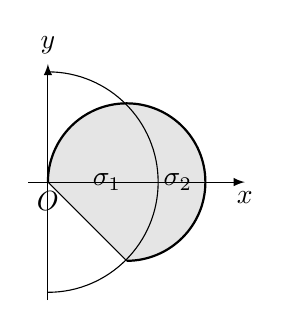
\begin{tikzpicture}[scale=1]
        \draw [black, thick, smooth, domain=0:1,fill=gray!20] (1,-1) arc (-90:180:1);
        \draw (0,0) -- (1,-1);
        \draw (0,-1.4) arc (-90:90:1.4);
        \draw[-latex](-0.25,0) -- (2.5,0) node[below]{$x$};
        \draw[-latex](0,-1.5) -- (0,1.5) node[above]{$y$};
        \filldraw[black] (0,0) node[below]{$O$};
        \filldraw (0.75,0) node{$\sigma_1$};
        \filldraw (1.65,0) node{$\sigma_2$};
    \end{tikzpicture}
\end{minipage}

$\sigma_1$的$r\in[0,\sqrt{2}]$,$\sigma_2$的$r\in[\sqrt{2},2]$。

$\sigma_1$的$\theta$下限是$y=-x$这条边,即$\theta=-\dfrac{\pi}{4}$,上限是$r=2\cos\theta$这个圆,则$\theta=\arccos\dfrac{r}{2}$。

$\sigma_2$的$\theta$界限都是是$r=2\cos\theta$这个圆,此时$r>0$恒成立,但是上限是上半部分$\theta>0$,而下限是下半部分$\theta<0$,即上限$\theta=\arccos\dfrac{r}{2}$,所以下限为$\theta=-\arccos\dfrac{r}{2}$。

综上交换积分次序结果为:

$\int_0^{\sqrt{2}}r\,\textrm{d}r\int_{-\frac{\pi}{4}}^{\arccos\frac{r}{2}}f(r\cos\theta,r\sin\theta)\textrm{d}\theta+\int_{\sqrt{2}}^2r\,\textrm{d}r\int_{-\arccos\frac{r}{2}}^{\arccos\frac{r}{2}}f(r\cos\theta,r\sin\theta)\textrm{d}\theta$。

\subsubsection{极直互化}

\textbf{例题:}将$I=\int_0^{\frac{\sqrt{2}}{2}R}e^{-y^2}\textrm{d}y\int_0^ye^{-x^2}\,\textrm{d}x+\int_{\frac{\sqrt{2}}{2}R}^Re^{-y^2}\,\textrm{d}y\int_0^{\sqrt{R^2-y^2}}e^{-x^2}\,\textrm{d}x$转换为极坐标系并计算结果。

解:首先根据积分上下限得到积分区域$D=\left\{0\leqslant y\leqslant\dfrac{\sqrt{2}}{2}R,0\leqslant x\leqslant y\right\}\cup\left\{\dfrac{\sqrt{2}}{2}R\leqslant y\leqslant R,0\leqslant x\leqslant\sqrt{R^2-y^2}\right\}$,$D$为一个八分之一圆的扇形。

根据$x=r\cos\theta$,$y=r\sin\theta$替换得到$D=\left\{(x,y)\bigg|0\leqslant r\leqslant R,\dfrac{\pi}{4}\leqslant\theta\leqslant\dfrac{\pi}{2}\right\}$。

又$e^{-y^2}\cdot e^{-x^2}=e^{-(x^2+y^2)}=e^{-r^2}$。

$\therefore I=\int_{\frac{\pi}{4}}^{\frac{\pi}{2}}\textrm{d}\theta\int_0^Re^{-r^2}r\,\textrm{d}r$。

\subsection{二重积分计算}

二重积分若是累次积分形式出现,则计算可以使用上面两种方法简便运算。

\subsubsection{交换积分次序}

主要用于直角坐标系。

当按照当前的积分次序无法算出时需要更换积分次序。主要是看$f(x,y)$是对$x$先积分更简单还是对$y$先积分更简单。

\textbf{例题:}求$\int_0^1\textrm{d}y\int_{\arcsin y}^{\pi-\arcsin y}\cos^2x\,\textrm{d}x$。

解:首先直接对这个式子直接计算,$\cos^2x=\dfrac{1}{2}(1+\cos2x)$,原式$=\dfrac{1}{2}\int_0^1(\pi-2y-\arcsin y)\textrm{d}y$。根本无法解出。

考虑交换积分次序,首先求$\sigma$,$y\in[0,1]$,$x\in[\arcsin y,\pi-\arcsin y]$,则$\sin x=y$,$y=\sin(\pi-x)=\sin x$即$x\in[0,\sin x]$。

将积分区域换成$X$型:$x\in[0,\pi]$,$y\in[0,\sin x]$。

$\int_0^\pi\cos^2x\,\textrm{d}x\int_0^{\sin x}\textrm{d}y=\int_0^\pi\cos^2x\sin x\,\textrm{d}x=-\int_0^\pi\cos^2x\,\textrm{d}(\cos x)=-\dfrac{\cos^3x}{3}\bigg|_0^\pi\\=\dfrac{2}{3}$。

\subsubsection{积分性质}

直角坐标系和极坐标系都可以使用。

\paragraph{直角坐标系} \leavevmode \medskip

主要是一般对称性(积分区域关于$x$轴对称若$y$奇则为0,关于$y$轴对称若$x$奇则为0)和轮换对称性(积分区域关于$y=x$对称则$xy$可以互换)。

\paragraph{极坐标系} \leavevmode \medskip

主要就是指一般对称性(画图可知)。

\textbf{例题:}求曲线$r^2=2ax^2\cos2\theta$($a>0$)所围图形面积。

解:即求$\iint\limits_D\textrm{d}x\textrm{d}y$。重点就是求$D$,已知$r$的表达式,要求$\theta$的取值范围。

又$r^2>0$,$x^2>0$,$a>0$,所以$\cos2\theta\geqslant0$,$-\dfrac{\pi}{4}\leqslant\theta\leqslant\dfrac{\pi}{4}$,$\dfrac{3\pi}{4}\leqslant\theta\leqslant\dfrac{5\pi}{4}$。

由对称性,所以$=4\int_0^{\frac{\pi}{4}}\textrm{d}\theta\int_0^{a\sqrt{2\cos2\theta}}r\,\textrm{d}r=4a^2\int_0^{\frac{\pi}{4}}\cos2\theta\,\textrm{d}\theta=2a^2$。

\subsubsection{切分区域}

主要用于直角坐标系转为极坐标系。

将不规则的区域划分为圆域。

\textbf{例题:}设$D=\{(x,y)|0\leqslant x\leqslant1,0\leqslant y\leqslant1\}$,求$\displaystyle{\iint\limits_D\dfrac{\textrm{d}x\textrm{d}y}{\sqrt{x^2+y^2}}}$。

解:由$f(x,y)=\dfrac{1}{\sqrt{x^2+y^2}}$,知道可以使用极坐标系来表示,但是$D$是一个正方形,无法用圆来简单表示。

又$D$可以从$y=x$切割为两个部分,所以令下三角形为$D_1$,$\displaystyle{\iint\limits_D\dfrac{\textrm{d}x\textrm{d}y}{\sqrt{x^2+y^2}}}=2\displaystyle{\iint\limits_{D_1}\dfrac{\textrm{d}x\textrm{d}y}{\sqrt{x^2+y^2}}}$。

所以$0\leqslant y$和$y=x$可以确定$\theta\in\left[0,\dfrac{\pi}{4}\right]$,$0\leqslant x\leqslant1$可以确定$r$上界为$x=1$,即$r\cos\theta=1$,即$r=\dfrac{1}{\cos\theta}$,确定$r\in\left[0,\dfrac{1}{\cos\theta}\right]$。

所以$=2\int_0^{\frac{\pi}{4}}\textrm{d}\theta\int_0^{\frac{1}{\cos\theta}}\textrm{d}r=2\int_0^{\frac{\pi}{4}}\dfrac{\textrm{d}\theta}{\cos\theta}=2\ln(\sec\theta+\tan\theta)|_0^{\frac{\pi}{4}}=2\ln(1+\sqrt{2})$。

即对二重积分求导,需要将二重积分化为一重积分。

\subsubsection{坐标轴移动}

主要用于直角坐标系转为极坐标系。

面对$D$为一个圆的部分区域,而圆心不在原点,则可以坐标轴移动让圆心到原点上,从而方便积分,本质就是换元。

\textbf{例题:}设积分区域$D=\{(x,y)\vert x^2+y^2\leqslant2x+2y\}$,求$\iint_D(x^2+xy+y^2)\textrm{d}\sigma$。

解:$D$为$(x-1)^2+(y-1)^2\leqslant\sqrt{2}$,即圆心在$(1,1)$的圆,极坐标系无法表示,所以必须平移坐标轴。

令$x-1=u$,$y-1=v$,$x=u+1$,$y=v+1$,此时$D'=\{(u,v)|u^2+v^2\leqslant2\}$。

$\iint\limits_D(x^2+xy+y^2)\textrm{d}\sigma=\iint\limits_{D'}[(u+1)^2+(u+1)(v+1)+(v+1)^2]\textrm{d}u\textrm{d}v=\iint\limits_{D'}[u^2+uv+v^2+3(u+v)+3]\textrm{d}u\textrm{d}v=\iint\limits_{D'}(u^2+v^2)\textrm{d}u\textrm{d}v+\iint\limits_{D'}[uv+3(u+v)]\textrm{d}u\textrm{d}v+3\iint_{D'}\textrm{d}u\textrm{d}v$。

由于$uv+3(u+v)$是关于$u$或$v$的奇函数,且$D'$关于$uv$轴都对称,所以积分值为0。且根据二重积分的几何意义$\iint\limits_{D'}\textrm{d}u\textrm{d}v=S_{D'}=2\pi$。

所以$\iint_D(x^2+xy+y^2)\textrm{d}\sigma=\iint\limits_{D'}(u^2+v^2)\textrm{d}u\textrm{d}v+6\pi$。

转换为极坐标系,$u=r\cos\theta$,$v=r\sin\theta$,则$D'=\{(r,\theta)|0\leqslant\theta\leqslant2\pi,0\leqslant r\leqslant\sqrt{2}\}$。

$\iint\limits_{D'}(u^2+v^2)\textrm{d}u\textrm{d}v=\int_0^{2\pi}\textrm{d}\theta\int_0^{\sqrt{2}}r^3\,\textrm{d}r=2\pi\int_0^{\sqrt{2}}r^3\,\textrm{d}r=\dfrac{\pi}{2}(\sqrt{2})^4=2\pi$。

所以原式$=2\pi+6\pi=8\pi$。

若积分区域$\sigma$关于$x=k_1$或$y=k_2$对称,则当$f(x,y)$含有$x-k_1$或$y-k_2$因式时重积分值为0。

\textbf{例题:}设$D:x^2+y^2\leqslant2x+2y$,求$\iint\limits_Dxy\,\textrm{d}x\textrm{d}y$。

解:本题目使用直角坐标系和极坐标系都不好做。所以需要利用积分性质,对$D$进行平移等操作。

利用平移,由于$D:(x-1)^2+(y-1)^2=2$,令$x=1+r\cos\theta$,$y=1+r\sin\theta$,则利用极坐标,$r\in[0,\sqrt{2}]$,$\theta\in[0,2\pi]$,$=\int_0^{2\pi}\textrm{d}\theta\int_0^{\sqrt{2}}((1+r\cos\theta)(1+r\sin\theta)r)\textrm{d}r=\int_0^{2\pi}\textrm{d}\theta\int_0^{\sqrt{2}}(1+r\sin\theta+r\cos\theta+r^2\sin\theta\cos\theta)r\,\textrm{d}r$,又将$\sin\theta$和$\cos\theta$对$\theta$在$[0,2\pi]$进行积分全部为0,所以直接把后面的全消掉,变为$\int_0^{2\pi}\textrm{d}\theta\int_0^{\sqrt{2}}r\,\textrm{d}r=2\pi$。

\subsubsection{极限化为二重积分}

类似极限转换为定积分,有$\lim\limits_{n\to\infty}\dfrac{1}{n^2}\sum\limits_{i=1}^n\sum\limits_{j=1}f\left(\dfrac{i}{n},\dfrac{j}{n}\right)=\int_0^1\textrm{d}x\int_0^1f(x,y)\,\textrm{d}y$:

\begin{enumerate}
    \item 先提出$\dfrac{1}{n^2}$。
    \item 凑出$\dfrac{i}{n}$和$\dfrac{j}{n}$。
    \item 写出$\int_0^1\textrm{d}x$、$\int_0^1f(x,y)\,\textrm{d}y$,其中$\dfrac{1}{n^2}$没有了,将所有$\dfrac{i}{n}$换为$x$,$\dfrac{j}{n}$换为$y$。
\end{enumerate}

\textbf{例题:}求$I=\lim\limits_{n\to\infty}\sum\limits_{i=1}^n\sum\limits_{j=1}^n\dfrac{1}{\left(1+\dfrac{i}{n}\right)(n^2+j^2)}$。

解:首先提出$\dfrac{1}{n^2}$,正好在分母右边等式中$=\lim\limits_{n\to\infty}\sum\limits_{i=1}^n\sum\limits_{j=1}^n\dfrac{1}{\left(1+\dfrac{i}{n}\right)(1+\dfrac{j^2}{n^2})}\dfrac{1}{n^2}$。

已完全化为$\dfrac{i}{n}$和$\dfrac{j}{n}$,所以$=\displaystyle{\int_0^1\dfrac{1}{1+x}\textrm{d}x\int_0^1\dfrac{1}{1+y^2}\textrm{d}y}$。

$=\ln(1+x)\vert_0^1\arctan y\vert_0^1=\dfrac{\pi}{4}\ln2$。

\subsubsection{二重积分极限}

即对存在二重积分的式子求极限。当对二重积分求极限时基本上都需要使用洛必达法则对积分求导。

令中间的定积分为$g(x)$,并记住$(\int_{f(x)}^{g(x)}h(t)\,\textrm{d}t)'=(g'(x)-f'(x))h(x)$。上下限最好换为$x$和$0$。

\textbf{例题:}求$\lim\limits_{t\to0^+}\dfrac{1}{t^6}\int_0^t\textrm{d}x\int_x^t\sin(xy)^2\textrm{d}y$。

解:这个式子求极限必然使用洛必达法则,而$\int_0^t\textrm{d}x\int_x^t\sin(xy)^2\textrm{d}y$里面那层定积分的上下限不规整,所以更换积分次序变成$\int_0^t\textrm{d}y\int_0^x\sin(xy)^2\textrm{d}x$。

对其求导$\int_0^t[\int_0^x\sin(xy)^2\textrm{d}x]\textrm{d}y$,由于该层积分变量为$y$,令$\int_0^x\sin(xy)^2\textrm{d}x=g(y)$,所以$=\int_0^tg(y)\,\textrm{d}y$,对其求导得$g(t)$,里面的$y$全部用$t$替换$=\int_0^x\sin(xt)^2\textrm{d}x$。

$=\lim\limits_{t\to0^+}\dfrac{\int_0^t\textrm{d}x\int_x^t\sin(xy)^2\textrm{d}y}{t^6}=\lim\limits_{t\to0^+}\dfrac{\int_0^t\sin(xt)^2\textrm{d}x}{6t^5}=\lim\limits_{t\to0^+}\dfrac{\int_0^t\sin(xt)^2\textrm{d}(xt)}{6t^6}$。

由于$x$和$t$都是变量,所以令$xt=u$,$x=\dfrac{u}{t}$,$u\in(0,t^2)$,$=\lim\limits_{t\to0^+}\dfrac{\int_0^{t^2}\sin u^2\textrm{d}u}{6t^6}=\lim\limits_{t\to0^+}\dfrac{2t\sin t^4}{36t^5}=\lim\limits_{t\to0^+}\dfrac{t^5}{18t^5}=\dfrac{1}{18}$。

\subsubsection{广义极坐标系}

广义极坐标系是对极坐标系的延伸,极坐标系是广义坐标系的特例。极坐标系是基于直线和圆周进行积分,而广义极坐标系可以对圆锥曲线进行积分。

当对面积为非圆形进行积分时可以使用广义极坐标系。

$\iint\limits_{D_1}f(x,y)\,\textrm{d}x\textrm{d}y$,$x=g(u,v)$,$y=h(u,v)$,换元为$\iint\limits_{D_2}f(g(u,v),h(u,v))\vert J\vert\,\textrm{d}u\textrm{d}v$,$J$为雅可比行列式,可以看作代表$(x,y)$坐标系的面积微元和$(u,v)$坐标系的面积微元的比率:

$J=\left[\begin{array}{cc}
    \dfrac{\partial x}{\partial u} & \dfrac{\partial x}{\partial v} \\
    \dfrac{\partial y}{\partial u} & \dfrac{\partial y}{\partial v}
\end{array}\right]$。

\textbf{例题:}设$D:\dfrac{x^2}{a}+\dfrac{y^2}{b}\leqslant1$,求$\iint\limits_Dy^2\,\textrm{d}x\textrm{d}y$。

解:令$x=ar\cos\theta$,$y=br\sin\theta$,所以$D'$为$0\leqslant r\leqslant 1$,$0\leqslant\theta\leqslant2\pi$。

变换雅可比行列式$J=\dfrac{\partial(x,y)}{\partial(r,\theta)}=\left\vert\begin{array}{cc}
    \dfrac{\partial x}{\partial r} & \dfrac{\partial x}{\partial\theta} \\
    \dfrac{\partial y}{\partial r} & \dfrac{\partial y}{\partial\theta}
\end{array}\right\vert=\left\vert\begin{array}{cc}
    a\cos\theta & -ar\sin\theta \\
    b\sin\theta & br\cos\theta
\end{array}\right\vert=abr$。

所以$I=\iint\limits_{D'}(br\sin\theta)^2\vert J\vert\,\textrm{d}r\textrm{d}\theta=\int_0^{2\pi}\textrm{d}\theta\int_0^1b^2r^2\sin^2\theta\cdot abr\,\textrm{d}r=\dfrac{\pi ab^3}{4}$。

\subsection{二重积分等式}

\subsubsection{函数}

\textbf{例题:}设$f(x,y)$为连续函数,且$f(x,y)=\dfrac{1}{\pi}\sqrt{x^2+y^2}\iint\limits_{x^2+y^2\leqslant1}f(x,y)\,\textrm{d}\sigma+y^2$,求$f(x,y)$。

解:$\because f(x,y)$为连续函数,所以其在区间上可积且是一个常数。

令$\iint\limits_{x^2+y^2\leqslant1}f(x,y)\,\textrm{d}\sigma=A$。对$f(x,y)=\dfrac{A}{\pi}\sqrt{x^2+y^2}+y^2$两边积分:

$A=\dfrac{A}{\pi}\iint\limits_{x^2+y^2\leqslant1}\sqrt{x^2+y^2}\,\textrm{d}\sigma+\iint\limits_{x^2+y^2\leqslant1}y^2\,\textrm{d}\sigma$,令$x=r\cos\theta$,$y=r\sin\theta$:

$A=\dfrac{A}{\pi}\int_0^{2\pi}\textrm{d}\theta\int_0^1r^2\,\textrm{d}r+\int_0^{2\pi}\sin^2\theta\textrm{d}\theta\int_0^1r^3\,\textrm{d}r=\dfrac{2A}{3}+\dfrac{\pi}{4}$。$A=\dfrac{3}{4}\pi$。

则代入原式$f(x,y)=\dfrac{3}{4}\sqrt{x^2+y^2}+y^2$。

\subsubsection{极限}

\textbf{例题:}设$g(x)$有连续的导数,且$g(0)=0$,$g'(0)=a\neq0$,$f(x,y)$在$(0,0)$的某邻域内连续,求$\lim\limits_{r\to0^+}\dfrac{\iint\limits_{x^2+y^2\leqslant r^2}f(x,y)\,\textrm{d}x\textrm{d}y}{g(r^2)}$。

解:已知对于这个积分式子中$f(x)$和$g(x)$都是未定式,不可能求出具体的值,所以不能再用二重积分直接计算。

面对这种未定式我们希望把这个式子变成我们已知的式子,也应该与$r$相关。此时我们可以想到二重积分中值定理。

根据二重积分中值定理$\iint\limits_{x^2+y^2\leqslant r^2}f(x,y)\,\textrm{d}x\textrm{d}y=\pi r^2f(\xi,\eta)$,其中$(\xi,\eta)$为圆域$x^2+y^2\leqslant r^2$上的点,所以$\lim\limits_{r\to0^+}f(\xi,\eta)=f(0,0)$。

$=\lim\limits_{r\to0^+}\dfrac{\pi r^2f(\xi,\eta)}{g(r^2)}=\lim\limits_{r\to0^+}\dfrac{\pi f(0,0)2r}{2rg'(r^2)}=\lim\limits_{r\to0^+}\dfrac{\pi f(0,0)}{g'(r^2)}=\dfrac{\pi f(0,0)}{g'(0)}=\dfrac{\pi f(0,0)}{a}$。

\subsubsection{求导}

\subsection{二重积分不等式}

即对二重积分进行对比。

\subsubsection{同积分域}

同一积分域上二重积分大小的比较,只要比较在该区间被积函数值的大小。

\subsubsection{同积分函数}

同一积分函数上二重积分大小的比较,要比较函数域的大小,也要注意在函数域上被积函数的符号。

\textbf{例题:}设积分区域$D_1=\{(x,y)|x^2+y^2\leqslant1\}$、$D_2=\{(x,y)|x^2+y^2\leqslant2\}$、$D_3=\left\{(x,y)|\dfrac{1}{2}x^2+y^2\leqslant1\right\}$、$D_4=\left\{(x,y)|x^2+\dfrac{1}{2}y^2\leqslant1\right\}$。\\记$I_i=\iint\limits_{D_i}\left[1-\left(x^2+\dfrac{1}{2}y^2\right)\right]\textrm{d}\sigma$($i=1,2,3,4$),求$\max\{I_1,I_2,I_3,I_4\}$。

解:已知$D_1$、$D_2$分别为半径1和$\sqrt{2}$的圆,而$D_3$、$D_4$分别为横着和竖着的椭圆。可以画出图像。

被积函数$f(x,y)=1-\left(x^2+\dfrac{1}{2}y^2\right)$为连续函数,只有在$D_4$上才能保证完全为正,以外的地方为负值。

所以$D_1\subset D_4$,所以$I_1<D_4$。对于$D_2$更大,$D_4\subset D_2$,但是多余的左右部分是负值,积分值会在$D_4$的基础上减去这部分的值,同理$D_3$和$D_4$一个是横的椭圆一个是竖的椭圆,其积分值只有中间交叉的部分,还要减去两边多余的部分。

所以$I_4$最大。

\subsection{一重积分化二重积分}

对于一重积分的计算或证明可能比较有难度,如两个关于$x$的函数的一重积分乘积计算,可以将其中一个$x$当作$y$,从而将一重积分的乘积变为二重积分。

\subsubsection{乘积化不等式}

\textbf{例题:}$f(x)$为恒大于0的连续函数,证明$\displaystyle{\int_a^bf(x)\,\textrm{d}x\cdot\int_a^b\dfrac{1}{f(x)}\textrm{d}x\geqslant(b-a)^2}$。

解:首先观察这个式子,右边是积分上下限的差的乘积,左边是两个积分的乘积,看上去貌似没什么关系,而且积分式子给出的是一个未定式$f(x)$,所以不能直接求左边值再比较大小,他们之间一定存在着某种关系。

式子左边的两个函数互为倒数,所以应该要尝试将这两个式子乘在一起来利用基本不等式计算,即将一重积分乘积变为二重积分。

对于一重积分而言只是一个自变量,对于二重积分而言就变成了两个自变量,需要令其中一个$f(x)$变为$y$,所以$xy$的积分区域都是一样的$[a,b]$,所以设$D=\{(x,y)\vert a\leqslant x\leqslant b,a\leqslant y\leqslant b\}$。

$I=\displaystyle{\int_a^bf(x)\,\textrm{d}x\cdot\int_a^b\dfrac{1}{f(x)}\textrm{d}x}=\int_a^bf(x)\,\textrm{d}x\cdot\int_a^b\dfrac{1}{f(y)}\textrm{d}y=\iint\limits_D\dfrac{f(x)}{f(y)}\textrm{d}x\textrm{d}y$。

$I=\displaystyle{\int_a^bf(x)\,\textrm{d}x\cdot\int_a^b\dfrac{1}{f(x)}\textrm{d}x}=\int_a^bf(y)\,\textrm{d}y\cdot\int_a^b\dfrac{1}{f(x)}\textrm{d}x=\iint\limits_D\dfrac{f(y)}{f(x)}\textrm{d}x\textrm{d}y$。

$\therefore I=\displaystyle{\dfrac{1}{2}\left[\iint\limits_D\left[\dfrac{f(x)}{f(y)}+\dfrac{f(y)}{f(x)}\right]\textrm{d}x\textrm{d}y\right]\geqslant\dfrac{1}{2}\iint\limits_D2\sqrt{\dfrac{f(x)}{f(y)}\cdot\dfrac{f(y)}{f(x)}}\textrm{d}x\textrm{d}y=}\\\displaystyle{\dfrac{1}{2}\iint\limits_D2\textrm{d}x\textrm{d}y}=(b-a)^2$。

\subsubsection{乘积简化计算}

\textbf{例题:}求$\int_0^{+\infty}e^{-x^2}\,\textrm{d}x$。

解:对于这个一重积分首先看到$e^{x^2}$,肯定会想到将其幂次降低。使用分部积分法对$e^{e^2}$求导这个幂次不会降低,使用换元法$x=\sqrt{t}$会得到$\dfrac{1}{\sqrt{t}}$从而无法处理,所以这些都不能计算,那么该怎么办?

看到$x^2$就能想到$x^2+y^2$的形式,这样就是一个极坐标系的二重积分,所以尝试将一重积分变成二重积分,即再乘一个以$y$为自变量的原式。

设$I=\int_0^{+\infty}e^{-x^2}\,\textrm{d}x$,显然$I>0$,将$x$换成$y$:

$I^2=\int_0^{+\infty}e^{-x^2}\,\textrm{d}x\cdot\int_0^{+\infty}e^{-x^2}\,\textrm{d}x=\int_0^{+\infty}e^{-x^2}\,\textrm{d}x\cdot\int_0^{+\infty}e^{-y^2}\,\textrm{d}y$

$=\displaystyle{\iint\limits_{\substack{0\leqslant x\leqslant+\infty\\0\leqslant y\leqslant+\infty}}e^{-(x^2+y^2)}\,\textrm{d}x\textrm{d}y}$,令$x=r\cos\theta$,$y=r\sin\theta$:

$=\displaystyle{\int_0^\frac{\pi}{2}\textrm{d}\theta\int_0^{+\infty}e^{-r^2}r\,\textrm{d}r=\dfrac{\pi}{2}\left(-\dfrac{1}{2}\right)\int_0^{+\infty}e^{-r^2}\,\textrm{d}(-r^2)=-\dfrac{\pi}{4}e^{-r^2}\bigg\vert_0^{+\infty}}=\dfrac{\pi}{4}$。

$\therefore I=\dfrac{\sqrt{\pi}}{2}$。

\subsection{二重积分应用}

\subsubsection{体积}

\subsubsection{形心公式}

直角坐标系和极坐标系的形心公式都是一样的,使用极坐标系可以转换。

\textbf{例题:}求曲线$ay=x^2$与$x+y=2a$所围平面区域$D$的形心坐标。

解:根据表达式可知有两个交点$(-2a,4a)$、$(a,a)$,形心公式:

$\overline{x}=\dfrac{\iint\limits_Dx\,\textrm{d}\sigma}{\iint\limits_D\textrm{d}\sigma}=\dfrac{\int_{-2a}^ax\,\textrm{d}x\int_{\frac{x^2}{a}}^{-x+2a}\textrm{d}y}{\int_{-2a}^a\,\textrm{d}x\int_{\frac{x^2}{a}}^{-x+2a}\textrm{d}y}=\dfrac{\int_{-2a}^a(-\dfrac{x^3}{a}-x^2+2ax)\textrm{d}x}{\int_{-2a}^a(-\dfrac{x^2}{a}-x+2a)\textrm{d}x}=-\dfrac{1}{2}a$

$\overline{y}=\dfrac{\iint\limits_Dy\,\textrm{d}\sigma}{\iint\limits_D\textrm{d}\sigma}=\dfrac{\int_{-2a}^a\,\textrm{d}x\int_{\frac{x^2}{a}}^{-x+2a}y\textrm{d}y}{\int_{-2a}^a\,\textrm{d}x\int_{\frac{x^2}{a}}^{-x+2a}\textrm{d}y}=\dfrac{\dfrac{1}{2}\int_{-2a}^a(-\dfrac{x^4}{4}+x^2-4ax+4a^2)}{\int_{-2a}^a(-\dfrac{x^2}{a}-x+2a)\textrm{d}x}=\dfrac{8}{5}a$

\section{弧长曲线积分}

\section{坐标曲线积分}

\subsection{定积分法}

\subsection{二重积分法}

\subsubsection{补全区域}

即$L$不能构成一个完整的域,就需要按照路径对区域进行补全,然后减去这个曲线积分值。

\subsubsection{不可导点}

即$D$中存在不可导的点,需要以不可导点为圆心做圆对$D$进行切割。

\textbf{例题:}$I=\displaystyle{\oint\limits_L\dfrac{x\textrm{d}y-y\textrm{d}}{x^2+y^2}}$,$L$为不过原点的闭曲线。

解:$P=-\dfrac{y}{x^2+y^2}$,$Q=\dfrac{x}{x^2+y^2}$。$\dfrac{\partial Q}{\partial x}=\dfrac{y^2-x^2}{(x^2+y^2)^2}$,$\dfrac{\partial P}{\partial y}=\dfrac{y^2-x^2}{(x^2+y^2)^2}$,从而$\dfrac{\partial Q}{\partial x}\equiv\dfrac{\partial P}{\partial y}$。但是此时$(x,y)\neq(0,0)$,所以格林公式无法使用。

若$(0,0)\notin D$,则可以使用格林公式,$I=\iint\limits_D0\,\textrm{d}\sigma=0$。

若$(0,0)\in D$,不可以使用格林公式,所以重新对$D$进行划分,令$L_0:x^2+y^2=r^2$,其中$r>0$且$L_0$不超过$D$,$L_0$为逆时针。中间的环为$D_1$,最里侧的圆为$D_2$。

所以对中间的环$D_1$使用格林公式:$\oint_{L+L_0^-}=\iint_{D_1}\left(\dfrac{\partial Q}{\partial x}-\dfrac{\partial P}{\partial y}\right)\textrm{d}\sigma=0$。

$\therefore\oint\limits_L+\oint\limits_{L_0^-}=\oint\limits_L-\oint\limits_{L_0}=0$,$\oint_L=\oint_{L_0}$。

$I=\displaystyle{\oint\limits_{L_0}\dfrac{x\textrm{d}y-y\textrm{d}x}{x^2+y^2}=\dfrac{1}{r^2}\oint\limits_{L_0}x\,\textrm{d}y-y\,\textrm{d}x=\dfrac{2}{r^2}\iint\limits_{D_2}\textrm{d}\sigma=2\pi}$。

\textbf{例题:}计算曲线积分$\oint\limits_L\dfrac{x\textrm{d}y-y\textrm{d}x}{4^x2+y^2}$,其中$L$是以点$(1,0)$为圆心,$R\geqslant1$为半径的圆,取逆时针方向。

解:由于是逆时针在$L$上,所以是正向:$=\displaystyle{\oint\limits_{L^+}\left(\dfrac{-y}{4x^2+y^2}\textrm{d}x+\dfrac{x}{4x^2+y^2}\textrm{d}y\right)}$。

又对于$L$所围成的圆面$D$,因为$4x^2+y^2\neq0$,所以$(0,0)$应该被挖去。

因为逆时针的方向下挖去这个点做的运动顺时针是负方向的,所以令其为$C^-$。

又因为格林公式$\oint\limits_{L^++C^-}P\,\textrm{d}x+Q\,\textrm{d}y=\displaystyle{\iint\limits_D\left(\dfrac{\partial Q}{\partial x}-\dfrac{\partial P}{\partial y}\right)\textrm{d}\sigma}=$\\$\displaystyle{\iint\limits_D\left(\dfrac{4x^2+y^2-3x^2}{(4x^2+y^2)^2}-\dfrac{-(4x^2+y^2)+2y^2}{(4x^2+y^2)^2}\right)\textrm{d}\sigma}=0$。旋度为0。

$=\oint\limits_{L^++C^-}-\oint\limits_{C^-}=0-\oint\limits_{C^-}=\oint\limits_{C^+}$。取$C:4x^2+y^2=\delta^2$,$\delta$为一个足够小的常数。(分母取$\delta^2$)

$=\displaystyle{\oint\limits_{C^+}\left(\dfrac{-y}{4x^2+y^2}\textrm{d}x+\dfrac{x}{4x^2+y^2}\textrm{d}y\right)}=\displaystyle{\oint\limits_{C^+}\left(\dfrac{-y}{\delta^2}\textrm{d}x+\dfrac{x}{\delta^2}\textrm{d}y\right)}$

$=\dfrac{1}{\delta^2}\oint\limits_{C^+}-y\,\textrm{d}x+x\,\textrm{d}y$,利用格林公式,$C^+$所成区域为$D'$:$\dfrac{1}{\delta^2}\oint\limits_{D'}(1-(-1))\,\textrm{d}\sigma=\dfrac{2}{\delta^2}D'=\dfrac{2}{\delta^2}\pi\dfrac{\delta}{2}\delta=\pi$。

\section{常数项级数}

\subsection{正项级数}

如果题目中没有说明,要首先证明多项式为正数,否则不能使用正项级数的方法。

\subsubsection{放缩法}

即根据收敛准则来进行判断。如果要判断原级数收敛,则辅助级数应该是对其放大,判断原级数发散,则辅助级数应该是对其缩小。

\subsubsection{比较判别法}

都需要找到一个好的级数进行比较。常用的只有两个:

$p$级数:$\sum\limits_{n=1}^\infty\dfrac{1}{n^p}\left\{\begin{array}{l}
    p>1, \text{收敛} \\
    p\leqslant1, \text{发散}
\end{array}\right.$。

等比级数(几何级数):$\sum\limits_{n=1}^\infty\dfrac{1}aq^{n-1}\left\{\begin{array}{l}
    \vert q\vert<1, \text{收敛} \\
    \vert q\vert\geqslant 1, \text{发散}
\end{array}\right.$。

当不知道用哪个时可以使用洛必达先计算一下极限值。

\subsubsection{比值判别法}

适用于含有$a^n$,$n!$,$n^n$的通项。主要是$n!$。

\textbf{例题:}判断$\sum\limits_{n=1}^\infty\dfrac{n!}{n^n}$。

解:利用比值判别法,令$a_n=\dfrac{n!}{n^n}$,$\lim\limits_{n\to\infty}\dfrac{a_{n+1}}{a_n}=\lim\limits_{n\to\infty}\dfrac{(n+1)!}{(n+1)^{n+1}}\dfrac{n^n}{n!}=\lim\limits_{n\to\infty}\dfrac{n^n}{(n+1)^n}$,注意这里幂也为变量,不是等于1而是上下同时除以$n^n$,$=\lim\limits_{n\to\infty}\dfrac{1}{(1+\frac{1}{n})^n}$,根据两个重要极限得到$=\dfrac{1}{e}<1$,所以收敛。

\subsubsection{根值判别法}

适用于含有$a^n$,$n^n$的通项。

$\lim\limits_{n\to\infty}\sqrt[n]{n}=1$。

\subsubsection{积分判别法}

\textbf{例题:}判断级数$\sum\limits_{n=2}^\infty\dfrac{1}{n\ln n}$的敛散性。

解:因为$\dfrac{1}{n\ln n}<\dfrac{1}{n}$,调和级数发散,所以比较判别法找不到一个较好的辅助级数。同理根据级数形式比值和根值判别法都无法使用。

令$f(x)=\dfrac{1}{x\ln x}$,$a_n=f(n)$,在$[2,+\infty)$上$\dfrac{1}{n\ln n}$单调减且非负。

级数$\sum\limits_{n=2}^\infty\dfrac{1}{n\ln n}$与$\int_2^{+\infty}\dfrac{\textrm{d}x}{x\ln x}$同敛散。

$=\ln\ln x\vert_2^{+\infty}=+\infty$,所以原级数发散。

\subsection{交错级数}

\section{幂级数}

\subsection{收敛域}

\subsubsection{基本方法}

使用比值或根值法进行求解。

\textbf{例题:}求幂级数$\sum\limits_{n=1}^\infty\dfrac{e^n-(-1)^n}{n^2}x^n$的收敛半径。

解:

比值法:

$\lim\limits_{n\to\infty}\left\vert\dfrac{a_{n+1}}{a_n}\right\vert=\lim\limits_{n\to\infty}\dfrac{e^{n+1}-(-1)^{n+1}}{(n+1)^2}\dfrac{n^2}{e^n-(-1)^n}=\lim\limits_{n\to\infty}\dfrac{e+(\frac{-1}{e})^n}{1-(\frac{-1}{e})^n}$。

又$\lim\limits_{n\to\infty}x^n=\left\{\begin{array}{ll}
    0 & \vert x\vert<1 \\
    \infty & \vert x\vert\geqslant1
\end{array}\right.$,$\lim\limits_{n\to\infty}\left(\dfrac{-1}{e}\right)^n=0$,原式$=e$。$R=\dfrac{1}{e}$。

根值法:

$\lim\limits_{n\to\infty}\sqrt[n]{\vert a_n\vert}=\lim\limits_{n\to\infty}\sqrt[n]{\dfrac{e^n-(-1)^n}{n^2}}=\lim\limits_{n\to\infty}\dfrac{e\sqrt[n]{1-(-\frac{-1}{e})^n}}{\sqrt[n]{n}\sqrt[n]{n}}$,又$\lim\limits_{n\to\infty}\sqrt[n]{n}=1$。

$=\lim\limits_{n\to\infty}\dfrac{e\sqrt[n]{1-0}}{1\cdot1}=e$,所以$R=\dfrac{1}{e}$。

\subsubsection{缺项变换}

若求$\sum\limits_{n=0}^\infty a_nx^{2n+1}$或$\sum\limits_{n=0}^\infty a_nx^{2n}$,则求出其$\rho$,$R=\sqrt{\dfrac{1}{\rho}}$。

\textbf{例题:}求幂级数$\sum\limits_{n=1}^\infty\dfrac{n}{2^n+(-3)^n}x^{2n-1}$的收敛半径。

解:由于分母都是幂函数,所以使用根值法:$=\lim\limits_{n=1}^\infty\sqrt[n]{\vert a_n\vert}=\lim\limits_{n=1}^\infty\dfrac{\sqrt[n]{n}}{\sqrt[n]{3^n+(-2)^n}}\\=\lim\limits_{n=1}^\infty\dfrac{1}{\sqrt[n]{1+(-\frac{2}{3})^n}}=\dfrac{1}{3}$。

所以$R=3$。注意这里是错误的,因为之前求收敛域时都是$x^n$,而这里是$x^{2n-1}$,只有奇数次项,所以幂级数的一半都没有了。

$\sum\limits_{n=1}^\infty a_nx^{2n}=\sum\limits_{n=1}^\infty a_nx^{2n-1}=\sum\limits_{n=1}^\infty a_n(x^2)^n$,当前已知收敛半径为$3$,即$\vert x^2\vert<3$,即$\vert x\vert<\sqrt{3}$。

\subsubsection{收敛域变换}

\textbf{例题:}已知幂级数$\sum\limits_{n=0}^\infty a_n(x+2)^n$在$x=0$处收敛,在$x=-4$处发散,求$\sum\limits_{n=0}^\infty a_n(x-3)^n$的收敛域。

解:根据阿贝尔定理,已知在$x=0$处收敛,且中心点在$x=-2$,则收敛区间为$(-4,0)$,在$x=-4$处发散,则$x<-4$,$x>0$处发散。

然后确定两端端点敛散性,$x=0$处收敛则收敛域包括$x=0$,$x=-4$处发散则收敛域不包括$x=-4$,得到收敛域$(-4,0]$。

对于$\sum\limits_{n=0}^\infty a_n(x-3)^n$的中心点为$x=3$,则根据相对位置收敛域为$(1,5]$。

\subsubsection{常数项级数变换}

可以代入特殊点确定收敛点,将幂级数转换为常数项级数。

\textbf{例题:}若级数$\sum\limits_{n=0}^\infty a_n$条件收敛,求幂级数$\sum\limits_{n=0}^\infty na_n(x-1)^n$的收敛区间。

解:已知$\sum\limits_{n=0}^\infty a_n$条件收敛,则对于幂级数$\sum\limits_{n=0}^\infty na_n(x-1)^n$而言在$x=2$处条件收敛,即得到以中心点$x=1$的收敛区间$(0,2)$。

\subsection{函数展开}

\subsubsection{因式分解}

\textbf{例题:}将函数$f(x)=\dfrac{1}{x^2-3x-4}$展开为$x-1$的幂级数并指出收敛区间。

解:$\dfrac{1}{x^2-3x-4}=\dfrac{1}{5}\left(\dfrac{1}{x-4}-\dfrac{1}{x+1}\right)$。

$\dfrac{1}{x-4}=\dfrac{1}{(x-1)-3}=-\dfrac{1}{3}\dfrac{1}{1-\frac{x-1}{3}}=-\dfrac{1}{3}\sum\limits_{n=0}^\infty\left(\dfrac{x-1}{3}\right)^n$,$\left\vert\dfrac{x-1}{3}\right\vert<1$,$x\in(-2,4)$。

$\dfrac{1}{x+1}=\dfrac{1}{(x-1)+2}=\dfrac{1}{2}\dfrac{1}{1+\frac{x-1}{2}}=\dfrac{1}{2}\sum\limits_{n=0}^\infty\left(-\dfrac{x-1}{2}\right)^n$,$\left\vert-\dfrac{x-1}{2}\right\vert<1$,$x\in(-1,3)$。

所以其幂级数就是其加和,收敛区间为$(-2,4)\cap(-1,3)=(-1,3)$。

\subsubsection{先导后积}

\textbf{例题:}求函数$f(x)=\arctan x$在$x=0$处的幂级数展开。

解:$f'(x)=(\arctan x)'=\dfrac{1}{1+x^2}=\dfrac{1}{1-(-x^2)}=\sum\limits_{n=0}^\infty(-1)^nx^{2n}$,$\vert-x^2\vert<1$。

已经求得求导后的函数的幂级数展开,所以求原函数的幂级数展开只需要积分,利用先导后积公式:$f(x)=f(0)+\int_0^xf'(t)\,\textrm{d}t=\int_0^x\sum\limits_{n=0}^\infty(-1)^nt^{2n}\,\textrm{d}t=\sum\limits_{n=0}^\infty(-1)^n\dfrac{t^{2n+1}}{2n+1}\bigg|_0^x=\sum\limits_{n=0}^\infty(-1)^n\dfrac{x^{2n+1}}{2n+1}$。

求导的级数要求$\vert x\vert<1$,代入$x=\pm1$到最后结果得到两个交错级数,所以收敛域其实为$[-1,1]$(可以不写)。

\subsection{级数求和}

即对展开式进行逆运算,根据幂级数展开式反推原幂级数。

可以利用展开式求和函数,但是很多展开式的通项都不是公式中的,就需要对通项进行变形。

在求和之前要先计算收敛半径和收敛域。

无论是哪个方法都要求求导和积分后系数$n+a$与幂次$n$相等,所以求导或积分的目的就是为了让他们相同,从而能被看成一个整体。

\subsubsection{先导后积}

$\sum\dfrac{x^{f(n)}}{P(n)}$:$n$在分母上,先导后积。使用变限积分:$\int_{x_0}^xS'(t)\,\textrm{d}t=S(x)-S(x_0)$,即$S(x)=S(x_0)+\int_{x_0}^xS'(t)\,\textrm{d}t$。一般选择$x_0$为展开点。

主要公式:$\sum\limits_{n=1}^\infty\dfrac{(-1)^{n-1}}{n}x^n=\ln(1+x)$($(-1,1]$);$\sum\limits_{n=1}^\infty\dfrac{x^n}{n}=-\ln(1-x)$($[-1,1)$)。

目的是让$P(n)=f(n)$。

% \textbf{例题:}求级数$\sum\limits_{n=1}^\infty\dfrac{x^n}{n}$的和函数。

% 解:已知$\sum\limits_{n=0}^\infty x^n=\dfrac{1}{1-x}$,而这里求和是$\dfrac{x^n}{n}$,所以需要对其进行转换。

% 对$\dfrac{x^n}{n}$求导就得到了$x^{n-1}$消去了分母的$n$,所以使用先导后积的方法。

% 记$S(x)=\sum\limits_{n=1}^\infty\dfrac{x^n}{n}$,则$x^n=(x-0)^n$,取$x_0=0$。

% $\therefore S(x)=S(0)+\displaystyle{\int_0^x\left(\sum\limits_{n=1}^\infty\dfrac{t^n}{n}\right)_t'\,\textrm{d}t}=0+\int_0^x(\sum\limits_{n=1}^\infty t^{n-1})\,\textrm{d}t=\displaystyle{\int_0^x\dfrac{1}{1-t}\textrm{d}t}=-\ln(1-x)$。收敛域为$[-1,1)$。

\textbf{例题:}求级数$\sum\limits_{n=0}^\infty\dfrac{(-1)^n}{2n+1}x^{2n}$的和函数。

解:首先$\lim\limits_{n\to\infty}\left\vert\dfrac{a_{n+1}}{a_n}\right\vert=1$,$R=1$。

当$x=\pm1$时,$x^2n=1$,所以原式$=\sum\limits_{n=0}^\infty\dfrac{(-1)^n}{2n+1}$,为交错级数,由莱布尼茨判别法可知极限为0且单调递减,从而该级数收敛。从而收敛域为$[-1,1]$。

令$S(x)=\sum\limits_{n=0}^\infty\dfrac{(-1)^n}{2n+1}x^{2n}$。易得$x=0$时$S(x)=1$。

当$x\neq0$时,$S(x)=\dfrac{1}{x}\sum\limits_{n=0}^\infty\dfrac{(-1)^n}{2n+1}x^{2n+1}=\dfrac{1}{x}\sum\limits_{n=0}^\infty\int_0^x(-1)^nx^{2n}\,\textrm{d}x\\=\dfrac{1}{x}\int_0^x[\sum\limits_{n=0}^\infty(-1)^nx^{2n}]\textrm{d}x$。

所以$(-1)^nx^{2n}$为一个几何级数,所以$q=\dfrac{(-1)^{n+1}x^{2n+2}}{(-1)^nx^{2n}}=-x^2$。

从而$=\displaystyle{\dfrac{1}{x}\int_0^x\dfrac{1}{1+x^2}\textrm{d}x=\dfrac{\arctan x}{x}}$。

\subsubsection{先积后导}

$\sum P(n)x^{f(n)}$:$n$在分子上,先积后导。$(\int S(x)\,\textrm{d}x)'=S(x)$。

主要公式:$\sum\limits_{n=0}^\infty(-1)^nx^n=\dfrac{1}{1+x}$($(-1,1)$);$\sum\limits_{n=0}^\infty x^n=\dfrac{1}{1-x}$($(-1,1)$)。

目的是让$P(n)=f^{(n)}(n)\cdots f'(n)$。

\textbf{例题:}求级数$\sum\limits_{n=1}^\infty nx^n$的和函数。

解:记$S(x)=\sum\limits_{n=1}^\infty nx^n=x\sum\limits_{n=1}^\infty x^{n-1}=x(\int\sum\limits_{n=1}^\infty nx^{n-1}\,\textrm{d}x)'=x(\sum\limits_{n=1}^\infty x^n)'=x\left(\dfrac{x}{1-x}\right)'=\dfrac{x}{(1-x)^2}$。收敛域为$[-1,1]$。

\textbf{例题:}求级数$\sum\limits_{n=0}^\infty(n+1)(n+3)x^n$的和函数。

解:$(n+1)(n+3)$的形式可以推出$(n+1)(n+2)$是求两次导的结果,而这里是$(n+1)(n+3)$,所以拆开:$\sum\limits_{n=0}^\infty(n+1)(n+2)x^n+\sum\limits_{n=0}^\infty(n+1)x^n=\left(\sum\limits_{n=0}^\infty x^{n+2}\right)''+\left(\sum\limits_{n=0}^\infty x^{n+1}\right)=\left(\dfrac{x^2}{1-x}\right)''+\left(\dfrac{x}{1-x}\right)'=\dfrac{3-x}{(1-x)^3}$,$x\in(-1,1)$。

\section{傅里叶级数}

\section{一阶微分方程}

\subsection{可分离变量微分方程}

\subsubsection{交叉积分法}

\textbf{例题:}求$y\sin\dfrac{x}{2}\,\textrm{d}x-\cos\dfrac{x}{2}\,\textrm{d}y=0$的通解。

解:$\dfrac{\textrm{d}y}{\textrm{d}x}=y\tan\dfrac{x}{2}$,$\dfrac{\textrm{d}y}{y}=\tan\dfrac{x}{2}\,\textrm{d}x$,$\displaystyle{\int\dfrac{\textrm{d}y}{y}=2\int\tan\dfrac{x}{2}\,\textrm{d}\dfrac{x}{2}}$。

解得$\ln\vert y\vert=-\ln\left(\cos\dfrac{x}{2}\right)^2+\ln C_1$(取对数更好解),$\vert y\vert=\dfrac{C_1}{\left(\cos\dfrac{x}{2}\right)^2}$。

$y=\dfrac{\pm C_1}{\left(\cos\dfrac{x}{2}\right)^2}$,令$C=\pm C_1$,得$y=\dfrac{C}{1+\cos x}$。

注意在第一步时将$y$除到分母上,本来$y$为任意常数,变为$y\neq0$,所以解得最后$C\neq0$,而实际上$y$可以为0,所以$C$应该为任意常数。

此时解为全部解,为通解加上$y=0$的奇解。

\subsubsection{多项式换元法}

$x$和$y$是以和差作为一个整体形式。

\textbf{例题:}求微分方程$\textrm{d}y=\sin(x+y+100)\,\textrm{d}x$的通解。

解:令$u=x+y+100$,$\dfrac{\textrm{d}u}{\textrm{d}x}=1+\dfrac{\textrm{d}y}{\textrm{d}x}$,$\dfrac{\textrm{d}y}{\textrm{d}x}=\sin(x+y+100)$,$\therefore\dfrac{\textrm{d}u}{\textrm{d}x}=1+\sin u$。

$\dfrac{\textrm{d}u}{1+\sin u}=\textrm{d}x$,$\displaystyle{\int\dfrac{\textrm{d}u}{1+\sin u}}=\int\textrm{d}x$,$\displaystyle{\int\dfrac{1-\sin u}{\cos^2u}}\textrm{d}u=x$。

$\int\sec^2u-\tan u\sec u\,\textrm{d}u=x$,即$\tan u-\sec u=x+C$。代回$u=x+y+100$:

通解$\tan(x+y+100)-\sec(x+y+100)=x+C$。

所有解:$\tan(x+y+100)-\sec(x+y+100)=x+C$,$x+y+100=2k\pi-\dfrac{\pi}{2}$。

\subsection{一阶线性方程}

形如$\dfrac{\textrm{d}y}{\textrm{d}x}+P(x)y=Q(x)$。

可以直接求也可以使用公式求。

\subsubsection{交叉积分法}

\textbf{例题:}设$L$是一条平面曲线,其上任意一点$P(x,y)$($x>0$)到坐标原点的距离恒等于该点处的切线在$y$轴上的截距,且$L$经过点$\left(\dfrac{1}{2},0\right)$,求$L$的方程。

解:$(x,y)$到坐标原点的距离为$\sqrt{x^2+y^2}$。

若$y=y(x)$,则切线为$Y-y=y'(X-x)$,令$X=0$,解得$Y=y-xy'$。

$\therefore\sqrt{x^2+y^2}=y-xy'$,解得$y'=\dfrac{\textrm{d}y}{\textrm{d}x}=\dfrac{y-\sqrt{x^2+y^2}}{x}=\dfrac{y}{x}-\sqrt{1+\dfrac{y^2}{x^2}}$。

令$\dfrac{y}{x}=u$,则$y=ux$,$\dfrac{\textrm{d}y}{\textrm{d}x}=\dfrac{\textrm{d}u}{\textrm{d}x}x+u$。代入$y'$:

$\dfrac{\textrm{d}u}{\textrm{d}x}x+u=u-\sqrt{1+u^2}$,$\dfrac{\textrm{d}u}{\sqrt{1+u^2}}=-\dfrac{\textrm{d}x}{x}$,$\displaystyle{\int\dfrac{\textrm{d}u}{\sqrt{1+u^2}}=-\int\dfrac{\textrm{d}x}{x}}$。

$\therefore\ln(u+\sqrt{1+u^2})=-\ln x+\ln C$,$u+\sqrt{1+u^2}=\dfrac{C}{x}$。

代入$\dfrac{y}{x}+\sqrt{1+\dfrac{y^2}{x^2}}=\dfrac{C}{x}$,$y+\sqrt{x^2+y^2}=C$。

\subsubsection{公式法}

即使用非齐次和非齐次的一阶线性微分方程公式。

\subsubsection{换元法}

如果存在$f(y)$,$y$无法提出,则使用换元法。典型的就是$e^y$。

\textbf{例题:}求微分方程$y'+1=e^{-y}\sin x$的通解。

解:已知对$e^{-y}\sin x$无法处理,所以必然需要对其转换,$e^yy'+e^y=\sin x$。

$\therefore(e^y)'+e^y=\sin x$,令$e^y=u$,$u'+u=\sin x$,$P(x)=1$,$Q(x)=\sin x$。

$e^y=u=e^{-\int\textrm{d}x}(\int e^{\int\textrm{d}x}\sin x\,\textrm{d}x+C)=e^{-x}(\int e^x\sin x\,\textrm{d}x+C)$,积分再现表格解出$\int e^x\sin x\,\textrm{d}x$:$=e^{-x}\left(\dfrac{1}{2}e^x(\sin x-\cos x)+C\right)$。

\textbf{例题:}求$y'=\dfrac{y^2-x}{2y(x+1)}$的通解。

解:这个式子首先分子分母等长,$xy$都合在一起,所以很难去分离出基本的微分方程。基本的微分方程式子为$y'+P(x)y=Q(x)$,对比可以看出里面$y^2$是不能化简的,所以很容易想到把这个当作一个整体。

$2y'y=\dfrac{y^2-x}{x+1}$,此时出现了$y^2$和$y^2$的导数,令$y^2=u$,$u'=\dfrac{u-x}{x+1}$。

即$u'-\dfrac{y}{x+1}=\dfrac{1}{x+1}-1$,此时就化为了一般非齐次方程。

根据公式算出$y=C(x+1)-(x+1)\ln\vert x+1\vert-1$。

\subsubsection{交换微分变量}

当出现$y'=\dfrac{f(x)}{g(x)}$,$g(x)$多项式的次数远高于$f(x)$,此时就没办法分离变量了,可以用$\dfrac{\textrm{d}x}{\textrm{d}y}$颠倒求导顺序。

\textbf{例题:}求$y'=\dfrac{y}{x+(y+1)^2}$的通解。($y$不为常函数)

解:由于$y'$对应的式子分母较复杂,而分子较简单,所以上下颠倒:

$\dfrac{\textrm{d}x}{\textrm{d}y}=\dfrac{x+(y+1)^2}{y}=\dfrac{x}{y}+y+\dfrac{1}{y}+2$。$x'-\dfrac{1}{y}x=y+\dfrac{1}{y}+2$。

根据公式:$x=e^{\int\frac{1}{y}\,\textrm{d}y}\left[\displaystyle{\int\left(y+\dfrac{1}{y}+2\right)}e^{\int-\frac{1}{y}\,\textrm{d}y}\,\textrm{d}y+C\right]=y^2+2\ln\vert y\vert y-1+Cy$。

\subsection{伯努利方程}

形如$\dfrac{\textrm{d}y}{\textrm{d}x}+P(x)y=Q(x)y^n$。

\textbf{例题:}求$y\,\textrm{d}x=(1+x\ln y)x\,\textrm{d}y$($y>0$)的通解。

解:将导数放到一边:$\dfrac{\textrm{d}y}{\textrm{d}x}=\dfrac{y}{(1+x\ln y)x}$,这个算式无法处理。

而颠倒$\dfrac{\textrm{d}x}{\textrm{d}y}=\dfrac{(1+x\ln y)x}{y}=\dfrac{1}{y}x+\dfrac{\ln y}{y}x^2$。

凑伯努利方程:$x'+P(x)x=Q(x)x^n$:$x'-\dfrac{1}{y}x=\dfrac{\ln y}{y}x^2$。$P(x)=-\dfrac{1}{y}$,$Q(x)=\dfrac{\ln y}{y}$。

乘$x^{-2}$降阶:$x^{-2}x'-\dfrac{1}{y}x^{-1}=\dfrac{\ln y}{y}$。令$z=x^{-1}$,$\dfrac{\textrm{d}z}{\textrm{d}y}=-\dfrac{1}{x^2}\dfrac{\textrm{d}x}{\textrm{d}y}$。代入方程:

$-\dfrac{\textrm{d}z}{\textrm{d}y}-\dfrac{1}{y}z=\dfrac{\ln y}{y}$,$\dfrac{\textrm{d}z}{\textrm{d}y}+\dfrac{1}{y}z=-\dfrac{\ln y}{y}$,利用公式:

$z=e^{-\int\frac{1}{y}\textrm{d}y}\left(\displaystyle{\int e^{\int\frac{1}{y}\textrm{d}y}\cdot\left(-\dfrac{\ln y}{y}\right)+C}\right)=\dfrac{1}{y}(-\int\ln y\,\textrm{d}y+C)=\dfrac{1}{y}(-y(\ln y-1)+C)=-\ln y+1+\dfrac{C}{y}$。

$\therefore x=\dfrac{y}{-y\ln y+y+C}$。

\section{二阶可降阶微分方程}

\subsection{\texorpdfstring{$y''=f(x,y')$}\ 型}

\textbf{例题:}求$y''=\dfrac{2xy'}{1+x^2}$的通解。

解:令$y'=p$,$p'=\dfrac{2xp}{1+x^2}$,$\dfrac{\textrm{d}p}{\textrm{d}x}=\dfrac{2xp}{1+x^2}$,$\dfrac{\textrm{d}p}{p}=\dfrac{2x}{1+x^2}$,$\displaystyle{\int\dfrac{\textrm{d}p}{p}=\int\dfrac{2x}{1+x^2}}$。

$\ln\vert p\vert=\ln(1+x^2)+\ln C_1$,$p=\pm C_1(1+x^2)=C_2(1+x^2)$。

$y'=C(1+x^2)$,$\therefore y=C_2\left(x+\dfrac{x^3}{3}+x\right)+C$。

\subsection{\texorpdfstring{$y''=f(y,y')$}\ 型}

\section{高阶线性微分方程}

% \subsection{常系数齐次线性微分方程}

% \subsection{常系数非齐次线性微分方程}

\subsection{二阶微分方程通解}

先将常系数非齐次线性微分方程变为常系数齐次线性微分方程求解,然后加上非齐次方程的一个特解,就是非齐次方程的一个通解。

特解只能拆为和的形式而不能拆为乘商的形式,如$Q(x)=\sin^2x$,则应该拆为$\dfrac{1-\cos2x}{2}$。

\textbf{例题:}求$y''-4y'+4y=3xe^{2x}$的通解。

解:变为常系数齐次线性微分方程:$y''-4y'+4y$。

写出特征方程:$\lambda^2-4\lambda+4=0$,从而$(\lambda-2)^2=0$,$\lambda_1=\lambda_2=2$。

从而$y$齐次方程的通解为$(C_1+C_2x)e^{2x}$。

根据特解的设置方法,所以$k=2$,设$y^*=e^{2x}(ax+b)x^2$。

代回二阶方程,$a=\dfrac{1}{2}$,$b=0$。通解为$(C_1+C_2x)e^{2x}+\dfrac{1}{2}x^3e^{2x}$。

\textbf{例题:}微分方程$y''-4y'+3y=e^x\cos x+xe^{3x}$的通解。

解:首先常系数齐次线性微分方程:$y''-4y'+3y=0$。

特征方程为$\lambda^2-4\lambda+3=0$,解得特征值为$\lambda_1=1$,$\lambda_2=3$。

所以该齐次方程的通解:$y=C_1e^x+C_2e^{3x}$。

然后求特解,首先求后面$f_2(x)=xe^{3x}$的特解$y_2^*$。

根据公式因为$\alpha$为单特征根,即$\aleph=3=\lambda_2\neq\lambda_1$,所以$y_2^*=e^{3x}(ax+b)x$。

然后是求$f_1(x)=e^x\cos x$的特解$y_1^*$。

其中$P_m(x)=1$,$P_n(x)=0$,$l=0$。所以设$P_m(x)=A$,$P_n(x)=B$。

对$k$,自由项中$\alpha=\beta=1$,得到$1\pm i$。又$1\pm i\neq\lambda_1=1\neq\lambda_2=3$,$k=0$。

最后$y_1^*=e^x(A\cos x+B\sin x)$。通解为$y=C_1e^x+C_2e^{3x}+e^x(A\cos x+B\sin x)+e^{3x}(ax+b)x$。

\subsection{反推微分方程}

\subsubsection{齐次微分方程}

没有给出具体的解出方法,此时往往是给出特解,然后反推微分方程的形式,这时就需要根据特解求出特征方程。

\textbf{例题:}计算具有特解$y_1=e^{-x}$、$y_2=2xe^{-x}$、$y_3=3e^x$的三阶常系数齐次线性微分方程。

解:由于是三阶,且不是一般的微分方程求特解而是逆问题,就使用特征方程解。

因为有三个特解,根据解的形式,$r=-1,-1,1$,所以特征方程的形式为$(r+1)^2(r-1)=0$,即解出$r^3+r^2-r-1=0$,所以微分方程为$y'''+y''-y'-y=0$。

\subsubsection{非齐次微分方程}

\paragraph{已知结构} \leavevmode \medskip

如果给出一个微分方程的具体形式,而携带参数,可以直接求导然后代入微分方程。

\textbf{例题:}$y=\dfrac{1}{2}e^{2x}+(x-\dfrac{1}{3})e^3$为二阶常系数非齐次线性微分方程$y''+ay'+by=ce^x$的一个特解,求对应参数。

解:直接代入法:直接求导$y'=e^{2x}+e^x(x+\dfrac{2}{3})$,$y''=2e^{2x}+e^x(x+\dfrac{5}{3})$。

直接代入,解得$a=-3$,$b=2$,$c=-1$。

\textbf{例题:}$y=e^{2x}+(x+1)e^x$为二阶常系数非齐次线性微分方程$y''+ay'+by=ce^x$的一个特解,求对应参数和通解。

解:解结构法:由于是二阶非齐次方程,所以必然是两个通解加一个特解。

展开解$y=e^{2x}+xe^x+e^x$。

由于已知解,所以$r=1$、$r=2$,且非齐次为$ce^x$,所以$e^2x$为齐次方程的一个通解,非齐次方程的特解必然是在$xe^x$和$e^x$之中。

由于$r=1$,$xe^x$和$e^x$的幂次都是$1$,而其中一个$r=1$,根据解的结构$Ae^{rx}x^k$,为单值根,所以$k=1$,所以特解必然存在$x^k$,所以$xe^x$为特解,$e^x$为通解。

所以特征方程为$(r-1)(r-2)=0$,对应$y''-3y'+2y=0$。然后直接代入求出$c$。

\paragraph{未知结构} \leavevmode \medskip

\textbf{例题:}已知二阶非齐次线性方程具有三个特解$y_1=x-(x^2+1)$、$y_2=3e^x-(x^2+1)$、$y_3=2x-e^x-(x^2+1)$,求$y(0)=y'(0)=0$的特解。

解:非齐次,即$y''+py'+qy=f(x)$。由于是二阶所以有两个无关的特解。

所以$y_1-y_2$,$y_1-y_3$为其齐次方程的两个通解(线性无关)。

通解为齐次方程通解加上非齐次一个特解:$y=C_1(y_1-y_2)+C_(y_1-y_3)+y_1$。

然后代入,解出$y=e^x-x^2-x-1$。

\subsection{高阶微分方程通解}

如果是三阶以及以上阶的微分方程,使用特征方程来解决。

由于三阶以以上的微分方程没有给出特解的形式,所以如果是高阶线性方程必然是齐次方程,直接根据特征方程得出特征值。

\textbf{例题:}求三阶常系数线性齐次微分方程$y'''-2y''+y'-2y=0$的通解。

解:得出特征方程$r^3-2r^2+r-2=0$,即$r^3-2r^2+r-2=0$,$(r-2)(r^2+1)=0$,解得$r=2$、$\pm i$,即得通解为$C_1e^{2x}+C_2\cos x+C_3\sin x$。

\section{微分方程概念}

对于有些方程并不需要求解后才能解决问题。

\subsection{已知微分方程的解反求系数}

\textbf{例题:}设$y_1,y_2$为一阶非齐次线性微分方程$y'+p(x)y=q(x)$的两个特解,若常数$\lambda,\mu$使得$\lambda y_1+\mu y_2$是该方程的解,$\lambda y_1-\mu y_2$是该方程对应的齐次方程的解,则()。

$A.\lambda=\dfrac{1}{2},\mu=\dfrac{1}{2}$\qquad$B.\lambda=-\dfrac{1}{2},\mu=-\dfrac{1}{2}$\qquad$C.\dfrac{2}{3},\mu=\dfrac{1}{3}$\qquad$\lambda=\dfrac{2}{3},\mu=\dfrac{2}{3}$

\subsection{不解微分方程,利用方程隐含信息}

$F(y,y',y'',\cdots,y^{(n)})=0$反映了\textbf{未知函数及其各阶导数之间的关系}。

\textbf{例题:}设$y=f(x)$是方程$y''-2y'+4y=0$的一个解,若$f(x_0)>0$,且$f'(x_0)=0$,则函数$f(x)$在点$x_0$()。

$A.$取得最大值\qquad$B.$取得最小值\qquad$C.$某个邻域内单调增加\qquad$D.$某个邻域内单调减少

解:因为$y=f(x)$是方程$y''-2y'+4y=0$的一个解,所以直接代入$x_0$:$y''(x_0)-2y'(x_0)+4y(x_0)=0$。又$f'(x_0)=0$。

$y''(x_0)=-4y(x_0)<0$,所以该点为极大值点。

\section{欧拉方程}

\section{微分方程物理应用}

\subsection{牛顿第二定律}

$F=ma$,物体质量$m$,力$f$,加速度$a=\dfrac{\textrm{d}^x}{\textrm{d}t^2}=\dfrac{\textrm{d}v}{\textrm{d}t}=\dfrac{\textrm{d}v}{\textrm{d}x}\dfrac{\textrm{d}x}{\textrm{d}t}=v\dfrac{\textrm{d}v}{\textrm{d}x}$。

\subsection{变化率}

考的可能性较大,提法多为$t$时刻某量$y$对$t$的变化率与$t$时刻某量成正比。

如冷却定律,$k$时刻物体温度$T(t)$对时间的变化率与$t$时刻物体与介质的温差$T-T_0$成正比,应写为$\dfrac{\textrm{d}T}{\textrm{d}t}=-k(x-x_0)$。

\end{document}
